\documentclass[pdflatex,sn-mathphys-ay]{sn-jnl}

\usepackage{amsmath,amssymb}
\usepackage{graphicx}
\graphicspath{{../figures/}}
\usepackage{booktabs}
\usepackage{multirow}
\usepackage{array}
\usepackage{enumitem}
\usepackage{microtype}
\usepackage{lineno}
\usepackage{placeins}
\usepackage{xr-hyper}
\externaldocument[S-]{RM_Precipitation_SERRA_supplement}
\usepackage{tikz}
\usetikzlibrary{arrows.meta,positioning}
% generated by code/serra/make_tables.py
\newcommand{\nsttexas}{40}
\newcommand{\nevtexas}{466}
\newcommand{\nstgermany}{40}
\newcommand{\nevgermany}{433}
\newcommand{\nstaustralia}{40}
\newcommand{\nevaustralia}{416}
\newcommand{\nsttaiwan}{13}
\newcommand{\nevtaiwan}{151}
\newcommand{\nstall}{133}
\newcommand{\nevall}{1466}
\newcommand{\qpathred}{\ensuremath{23.5}}
\newcommand{\msediffloall}{\ensuremath{-0.11}}
\newcommand{\msediffhiall}{\ensuremath{-0.04}}
\newcommand{\msediffgruloall}{\ensuremath{-0.06}}
\newcommand{\msediffgruhiall}{\ensuremath{+0.04}}
\newcommand{\tostmax}{3.9\times10^{-10}}
\newcommand{\msssmin}{\ensuremath{0.054}}
\newcommand{\msssmax}{\ensuremath{0.176}}
\newcommand{\chancetexasDone}{\ensuremath{0.509}}
\newcommand{\chancelotexasDone}{\ensuremath{0.467}}
\newcommand{\chancehitexasDone}{\ensuremath{0.552}}
\newcommand{\chancetexasDtwo}{\ensuremath{0.496}}
\newcommand{\chancelotexasDtwo}{\ensuremath{0.448}}
\newcommand{\chancehitexasDtwo}{\ensuremath{0.541}}
\newcommand{\chancetexasDthree}{\ensuremath{0.500}}
\newcommand{\chancelotexasDthree}{\ensuremath{0.459}}
\newcommand{\chancehitexasDthree}{\ensuremath{0.541}}
\newcommand{\chancetexasDfour}{\ensuremath{0.521}}
\newcommand{\chancelotexasDfour}{\ensuremath{0.482}}
\newcommand{\chancehitexasDfour}{\ensuremath{0.556}}
\newcommand{\chancetexasDfive}{\ensuremath{0.442}}
\newcommand{\chancelotexasDfive}{\ensuremath{0.406}}
\newcommand{\chancehitexasDfive}{\ensuremath{0.476}}
\newcommand{\chancetexasDseven}{\ensuremath{0.531}}
\newcommand{\chancelotexasDseven}{\ensuremath{0.489}}
\newcommand{\chancehitexasDseven}{\ensuremath{0.575}}
\newcommand{\chancetexasDsix}{\ensuremath{0.504}}
\newcommand{\chancelotexasDsix}{\ensuremath{0.460}}
\newcommand{\chancehitexasDsix}{\ensuremath{0.547}}
\newcommand{\podtexasDone}{\ensuremath{0.708}}
\newcommand{\fartexasDone}{\ensuremath{0.93}}
\newcommand{\timtexasDone}{\ensuremath{+16}}
\newcommand{\podtexasDtwo}{\ensuremath{0.687}}
\newcommand{\fartexasDtwo}{\ensuremath{0.94}}
\newcommand{\timtexasDtwo}{\ensuremath{+15}}
\newcommand{\podtexasDthree}{\ensuremath{0.809}}
\newcommand{\fartexasDthree}{\ensuremath{0.85}}
\newcommand{\timtexasDthree}{\ensuremath{+30}}
\newcommand{\podtexasDfour}{\ensuremath{0.809}}
\newcommand{\fartexasDfour}{\ensuremath{0.93}}
\newcommand{\timtexasDfour}{\ensuremath{+25}}
\newcommand{\podtexasDfive}{\ensuremath{0.358}}
\newcommand{\fartexasDfive}{\ensuremath{1.22}}
\newcommand{\timtexasDfive}{\ensuremath{+47}}
\newcommand{\podtexasDseven}{\ensuremath{0.794}}
\newcommand{\fartexasDseven}{\ensuremath{0.93}}
\newcommand{\timtexasDseven}{\ensuremath{+14}}
\newcommand{\podtexasDsix}{\ensuremath{0.790}}
\newcommand{\fartexasDsix}{\ensuremath{0.88}}
\newcommand{\timtexasDsix}{\ensuremath{+23}}
\newcommand{\chancegermanyDone}{\ensuremath{0.453}}
\newcommand{\chancelogermanyDone}{\ensuremath{0.413}}
\newcommand{\chancehigermanyDone}{\ensuremath{0.494}}
\newcommand{\chancegermanyDtwo}{\ensuremath{0.453}}
\newcommand{\chancelogermanyDtwo}{\ensuremath{0.408}}
\newcommand{\chancehigermanyDtwo}{\ensuremath{0.498}}
\newcommand{\chancegermanyDthree}{\ensuremath{0.428}}
\newcommand{\chancelogermanyDthree}{\ensuremath{0.386}}
\newcommand{\chancehigermanyDthree}{\ensuremath{0.469}}
\newcommand{\chancegermanyDfour}{\ensuremath{0.498}}
\newcommand{\chancelogermanyDfour}{\ensuremath{0.455}}
\newcommand{\chancehigermanyDfour}{\ensuremath{0.540}}
\newcommand{\chancegermanyDfive}{\ensuremath{0.505}}
\newcommand{\chancelogermanyDfive}{\ensuremath{0.465}}
\newcommand{\chancehigermanyDfive}{\ensuremath{0.550}}
\newcommand{\chancegermanyDseven}{\ensuremath{0.442}}
\newcommand{\chancelogermanyDseven}{\ensuremath{0.400}}
\newcommand{\chancehigermanyDseven}{\ensuremath{0.485}}
\newcommand{\chancegermanyDsix}{\ensuremath{0.442}}
\newcommand{\chancelogermanyDsix}{\ensuremath{0.401}}
\newcommand{\chancehigermanyDsix}{\ensuremath{0.487}}
\newcommand{\podgermanyDone}{\ensuremath{0.633}}
\newcommand{\fargermanyDone}{\ensuremath{0.84}}
\newcommand{\timgermanyDone}{\ensuremath{+0}}
\newcommand{\podgermanyDtwo}{\ensuremath{0.619}}
\newcommand{\fargermanyDtwo}{\ensuremath{0.83}}
\newcommand{\timgermanyDtwo}{\ensuremath{+1}}
\newcommand{\podgermanyDthree}{\ensuremath{0.739}}
\newcommand{\fargermanyDthree}{\ensuremath{0.66}}
\newcommand{\timgermanyDthree}{\ensuremath{+26}}
\newcommand{\podgermanyDfour}{\ensuremath{0.349}}
\newcommand{\fargermanyDfour}{\ensuremath{1.18}}
\newcommand{\timgermanyDfour}{\ensuremath{-1}}
\newcommand{\podgermanyDfive}{\ensuremath{0.413}}
\newcommand{\fargermanyDfive}{\ensuremath{1.24}}
\newcommand{\timgermanyDfive}{\ensuremath{+34}}
\newcommand{\podgermanyDseven}{\ensuremath{0.753}}
\newcommand{\fargermanyDseven}{\ensuremath{0.72}}
\newcommand{\timgermanyDseven}{\ensuremath{+9}}
\newcommand{\podgermanyDsix}{\ensuremath{0.727}}
\newcommand{\fargermanyDsix}{\ensuremath{0.70}}
\newcommand{\timgermanyDsix}{\ensuremath{+17}}
\newcommand{\chanceaustraliaDone}{\ensuremath{0.470}}
\newcommand{\chanceloaustraliaDone}{\ensuremath{0.430}}
\newcommand{\chancehiaustraliaDone}{\ensuremath{0.513}}
\newcommand{\chanceaustraliaDtwo}{\ensuremath{0.496}}
\newcommand{\chanceloaustraliaDtwo}{\ensuremath{0.457}}
\newcommand{\chancehiaustraliaDtwo}{\ensuremath{0.538}}
\newcommand{\chanceaustraliaDthree}{\ensuremath{0.489}}
\newcommand{\chanceloaustraliaDthree}{\ensuremath{0.448}}
\newcommand{\chancehiaustraliaDthree}{\ensuremath{0.534}}
\newcommand{\chanceaustraliaDfour}{\ensuremath{0.419}}
\newcommand{\chanceloaustraliaDfour}{\ensuremath{0.380}}
\newcommand{\chancehiaustraliaDfour}{\ensuremath{0.459}}
\newcommand{\chanceaustraliaDfive}{\ensuremath{0.261}}
\newcommand{\chanceloaustraliaDfive}{\ensuremath{0.231}}
\newcommand{\chancehiaustraliaDfive}{\ensuremath{0.293}}
\newcommand{\chanceaustraliaDseven}{\ensuremath{0.464}}
\newcommand{\chanceloaustraliaDseven}{\ensuremath{0.419}}
\newcommand{\chancehiaustraliaDseven}{\ensuremath{0.510}}
\newcommand{\chanceaustraliaDsix}{\ensuremath{0.507}}
\newcommand{\chanceloaustraliaDsix}{\ensuremath{0.454}}
\newcommand{\chancehiaustraliaDsix}{\ensuremath{0.550}}
\newcommand{\podaustraliaDone}{\ensuremath{0.712}}
\newcommand{\faraustraliaDone}{\ensuremath{0.83}}
\newcommand{\timaustraliaDone}{\ensuremath{+12}}
\newcommand{\podaustraliaDtwo}{\ensuremath{0.731}}
\newcommand{\faraustraliaDtwo}{\ensuremath{0.87}}
\newcommand{\timaustraliaDtwo}{\ensuremath{+12}}
\newcommand{\podaustraliaDthree}{\ensuremath{0.812}}
\newcommand{\faraustraliaDthree}{\ensuremath{0.85}}
\newcommand{\timaustraliaDthree}{\ensuremath{+22}}
\newcommand{\podaustraliaDfour}{\ensuremath{0.325}}
\newcommand{\faraustraliaDfour}{\ensuremath{0.93}}
\newcommand{\timaustraliaDfour}{\ensuremath{-6}}
\newcommand{\podaustraliaDfive}{\ensuremath{0.221}}
\newcommand{\faraustraliaDfive}{\ensuremath{0.70}}
\newcommand{\timaustraliaDfive}{\ensuremath{+63}}
\newcommand{\podaustraliaDseven}{\ensuremath{0.760}}
\newcommand{\faraustraliaDseven}{\ensuremath{0.76}}
\newcommand{\timaustraliaDseven}{\ensuremath{+18}}
\newcommand{\podaustraliaDsix}{\ensuremath{0.851}}
\newcommand{\faraustraliaDsix}{\ensuremath{0.87}}
\newcommand{\timaustraliaDsix}{\ensuremath{+16}}
\newcommand{\chancetaiwanDone}{\ensuremath{0.330}}
\newcommand{\chancelotaiwanDone}{\ensuremath{0.265}}
\newcommand{\chancehitaiwanDone}{\ensuremath{0.397}}
\newcommand{\chancetaiwanDtwo}{\ensuremath{0.340}}
\newcommand{\chancelotaiwanDtwo}{\ensuremath{0.278}}
\newcommand{\chancehitaiwanDtwo}{\ensuremath{0.397}}
\newcommand{\chancetaiwanDthree}{\ensuremath{0.383}}
\newcommand{\chancelotaiwanDthree}{\ensuremath{0.311}}
\newcommand{\chancehitaiwanDthree}{\ensuremath{0.457}}
\newcommand{\chancetaiwanDfour}{\ensuremath{0.430}}
\newcommand{\chancelotaiwanDfour}{\ensuremath{0.358}}
\newcommand{\chancehitaiwanDfour}{\ensuremath{0.497}}
\newcommand{\chancetaiwanDfive}{\ensuremath{0.427}}
\newcommand{\chancelotaiwanDfive}{\ensuremath{0.371}}
\newcommand{\chancehitaiwanDfive}{\ensuremath{0.490}}
\newcommand{\chancetaiwanDseven}{\ensuremath{0.375}}
\newcommand{\chancelotaiwanDseven}{\ensuremath{0.305}}
\newcommand{\chancehitaiwanDseven}{\ensuremath{0.444}}
\newcommand{\chancetaiwanDsix}{\ensuremath{0.346}}
\newcommand{\chancelotaiwanDsix}{\ensuremath{0.278}}
\newcommand{\chancehitaiwanDsix}{\ensuremath{0.411}}
\newcommand{\podtaiwanDone}{\ensuremath{0.497}}
\newcommand{\fartaiwanDone}{\ensuremath{0.61}}
\newcommand{\timtaiwanDone}{\ensuremath{+7}}
\newcommand{\podtaiwanDtwo}{\ensuremath{0.450}}
\newcommand{\fartaiwanDtwo}{\ensuremath{0.67}}
\newcommand{\timtaiwanDtwo}{\ensuremath{+10}}
\newcommand{\podtaiwanDthree}{\ensuremath{0.550}}
\newcommand{\fartaiwanDthree}{\ensuremath{0.70}}
\newcommand{\timtaiwanDthree}{\ensuremath{+33}}
\newcommand{\podtaiwanDfour}{\ensuremath{0.556}}
\newcommand{\fartaiwanDfour}{\ensuremath{0.82}}
\newcommand{\timtaiwanDfour}{\ensuremath{+30}}
\newcommand{\podtaiwanDfive}{\ensuremath{0.424}}
\newcommand{\fartaiwanDfive}{\ensuremath{1.02}}
\newcommand{\timtaiwanDfive}{\ensuremath{+24}}
\newcommand{\podtaiwanDseven}{\ensuremath{0.523}}
\newcommand{\fartaiwanDseven}{\ensuremath{0.70}}
\newcommand{\timtaiwanDseven}{\ensuremath{+17}}
\newcommand{\podtaiwanDsix}{\ensuremath{0.543}}
\newcommand{\fartaiwanDsix}{\ensuremath{0.60}}
\newcommand{\timtaiwanDsix}{\ensuremath{+29}}
\newcommand{\chanceallDone}{\ensuremath{0.463}}
\newcommand{\chanceloallDone}{\ensuremath{0.442}}
\newcommand{\chancehiallDone}{\ensuremath{0.486}}
\newcommand{\chanceallDtwo}{\ensuremath{0.467}}
\newcommand{\chanceloallDtwo}{\ensuremath{0.444}}
\newcommand{\chancehiallDtwo}{\ensuremath{0.489}}
\newcommand{\chanceallDthree}{\ensuremath{0.463}}
\newcommand{\chanceloallDthree}{\ensuremath{0.441}}
\newcommand{\chancehiallDthree}{\ensuremath{0.488}}
\newcommand{\chanceallDfour}{\ensuremath{0.476}}
\newcommand{\chanceloallDfour}{\ensuremath{0.454}}
\newcommand{\chancehiallDfour}{\ensuremath{0.496}}
\newcommand{\chanceallDfive}{\ensuremath{0.408}}
\newcommand{\chanceloallDfive}{\ensuremath{0.386}}
\newcommand{\chancehiallDfive}{\ensuremath{0.428}}
\newcommand{\chanceallDseven}{\ensuremath{0.470}}
\newcommand{\chanceloallDseven}{\ensuremath{0.447}}
\newcommand{\chancehiallDseven}{\ensuremath{0.493}}
\newcommand{\chanceallDsix}{\ensuremath{0.470}}
\newcommand{\chanceloallDsix}{\ensuremath{0.447}}
\newcommand{\chancehiallDsix}{\ensuremath{0.494}}
\newcommand{\podallDone}{\ensuremath{0.665}}
\newcommand{\farallDone}{\ensuremath{0.84}}
\newcommand{\timallDone}{\ensuremath{+8}}
\newcommand{\podallDtwo}{\ensuremath{0.655}}
\newcommand{\farallDtwo}{\ensuremath{0.86}}
\newcommand{\timallDtwo}{\ensuremath{+9}}
\newcommand{\podallDthree}{\ensuremath{0.763}}
\newcommand{\farallDthree}{\ensuremath{0.78}}
\newcommand{\timallDthree}{\ensuremath{+27}}
\newcommand{\podallDfour}{\ensuremath{0.510}}
\newcommand{\farallDfour}{\ensuremath{0.99}}
\newcommand{\timallDfour}{\ensuremath{+14}}
\newcommand{\podallDfive}{\ensuremath{0.342}}
\newcommand{\farallDfive}{\ensuremath{1.04}}
\newcommand{\timallDfive}{\ensuremath{+43}}
\newcommand{\podallDseven}{\ensuremath{0.744}}
\newcommand{\farallDseven}{\ensuremath{0.79}}
\newcommand{\timallDseven}{\ensuremath{+13}}
\newcommand{\podallDsix}{\ensuremath{0.763}}
\newcommand{\farallDsix}{\ensuremath{0.80}}
\newcommand{\timallDsix}{\ensuremath{+20}}
\newcommand{\dpodtexasDoneDtwo}{\ensuremath{+0.021}}
\newcommand{\dpodlotexasDoneDtwo}{\ensuremath{-0.018}}
\newcommand{\dpodhitexasDoneDtwo}{\ensuremath{+0.054}}
\newcommand{\dfartexasDoneDtwo}{\ensuremath{-0.01}}
\newcommand{\dfarlotexasDoneDtwo}{\ensuremath{-0.04}}
\newcommand{\dfarhitexasDoneDtwo}{\ensuremath{+0.02}}
\newcommand{\dtimtexasDoneDtwo}{\ensuremath{0}}
\newcommand{\dtimlotexasDoneDtwo}{\ensuremath{-1}}
\newcommand{\dtimhitexasDoneDtwo}{\ensuremath{0}}
\newcommand{\fearlytexasDoneDtwo}{\ensuremath{41}}
\newcommand{\dpodtexasDoneDthree}{\ensuremath{-0.101}}
\newcommand{\dpodlotexasDoneDthree}{\ensuremath{-0.188}}
\newcommand{\dpodhitexasDoneDthree}{\ensuremath{-0.024}}
\newcommand{\dfartexasDoneDthree}{\ensuremath{+0.08}}
\newcommand{\dfarlotexasDoneDthree}{\ensuremath{-0.07}}
\newcommand{\dfarhitexasDoneDthree}{\ensuremath{+0.23}}
\newcommand{\dtimtexasDoneDthree}{\ensuremath{16}}
\newcommand{\dtimlotexasDoneDthree}{\ensuremath{8.5}}
\newcommand{\dtimhitexasDoneDthree}{\ensuremath{23}}
\newcommand{\fearlytexasDoneDthree}{\ensuremath{66}}
\newcommand{\dpodtexasDoneDfour}{\ensuremath{-0.101}}
\newcommand{\dpodlotexasDoneDfour}{\ensuremath{-0.172}}
\newcommand{\dpodhitexasDoneDfour}{\ensuremath{-0.034}}
\newcommand{\dfartexasDoneDfour}{\ensuremath{+0.00}}
\newcommand{\dfarlotexasDoneDfour}{\ensuremath{-0.16}}
\newcommand{\dfarhitexasDoneDfour}{\ensuremath{+0.18}}
\newcommand{\dtimtexasDoneDfour}{\ensuremath{9}}
\newcommand{\dtimlotexasDoneDfour}{\ensuremath{3}}
\newcommand{\dtimhitexasDoneDfour}{\ensuremath{15}}
\newcommand{\fearlytexasDoneDfour}{\ensuremath{60}}
\newcommand{\dpodtexasDoneDseven}{\ensuremath{-0.086}}
\newcommand{\dpodlotexasDoneDseven}{\ensuremath{-0.165}}
\newcommand{\dpodhitexasDoneDseven}{\ensuremath{-0.014}}
\newcommand{\dfartexasDoneDseven}{\ensuremath{-0.00}}
\newcommand{\dfarlotexasDoneDseven}{\ensuremath{-0.10}}
\newcommand{\dfarhitexasDoneDseven}{\ensuremath{+0.09}}
\newcommand{\dtimtexasDoneDseven}{\ensuremath{3}}
\newcommand{\dtimlotexasDoneDseven}{\ensuremath{0}}
\newcommand{\dtimhitexasDoneDseven}{\ensuremath{5}}
\newcommand{\fearlytexasDoneDseven}{\ensuremath{56}}
\newcommand{\dpodtexasDsevenDthree}{\ensuremath{-0.015}}
\newcommand{\dpodlotexasDsevenDthree}{\ensuremath{-0.051}}
\newcommand{\dpodhitexasDsevenDthree}{\ensuremath{+0.023}}
\newcommand{\dfartexasDsevenDthree}{\ensuremath{+0.08}}
\newcommand{\dfarlotexasDsevenDthree}{\ensuremath{-0.04}}
\newcommand{\dfarhitexasDsevenDthree}{\ensuremath{+0.20}}
\newcommand{\dtimtexasDsevenDthree}{\ensuremath{18}}
\newcommand{\dtimlotexasDsevenDthree}{\ensuremath{16}}
\newcommand{\dtimhitexasDsevenDthree}{\ensuremath{23}}
\newcommand{\fearlytexasDsevenDthree}{\ensuremath{74}}
\newcommand{\dpodtexasDsixDthree}{\ensuremath{-0.019}}
\newcommand{\dpodlotexasDsixDthree}{\ensuremath{-0.057}}
\newcommand{\dpodhitexasDsixDthree}{\ensuremath{+0.019}}
\newcommand{\dfartexasDsixDthree}{\ensuremath{+0.02}}
\newcommand{\dfarlotexasDsixDthree}{\ensuremath{-0.02}}
\newcommand{\dfarhitexasDsixDthree}{\ensuremath{+0.07}}
\newcommand{\dtimtexasDsixDthree}{\ensuremath{4}}
\newcommand{\dtimlotexasDsixDthree}{\ensuremath{3}}
\newcommand{\dtimhitexasDsixDthree}{\ensuremath{5}}
\newcommand{\fearlytexasDsixDthree}{\ensuremath{70}}
\newcommand{\dpodgermanyDoneDtwo}{\ensuremath{+0.014}}
\newcommand{\dpodlogermanyDoneDtwo}{\ensuremath{-0.013}}
\newcommand{\dpodhigermanyDoneDtwo}{\ensuremath{+0.042}}
\newcommand{\dfargermanyDoneDtwo}{\ensuremath{+0.00}}
\newcommand{\dfarlogermanyDoneDtwo}{\ensuremath{-0.05}}
\newcommand{\dfarhigermanyDoneDtwo}{\ensuremath{+0.05}}
\newcommand{\dtimgermanyDoneDtwo}{\ensuremath{1}}
\newcommand{\dtimlogermanyDoneDtwo}{\ensuremath{0}}
\newcommand{\dtimhigermanyDoneDtwo}{\ensuremath{1}}
\newcommand{\fearlygermanyDoneDtwo}{\ensuremath{51}}
\newcommand{\dpodgermanyDoneDthree}{\ensuremath{-0.106}}
\newcommand{\dpodlogermanyDoneDthree}{\ensuremath{-0.188}}
\newcommand{\dpodhigermanyDoneDthree}{\ensuremath{-0.019}}
\newcommand{\dfargermanyDoneDthree}{\ensuremath{+0.18}}
\newcommand{\dfarlogermanyDoneDthree}{\ensuremath{+0.02}}
\newcommand{\dfarhigermanyDoneDthree}{\ensuremath{+0.34}}
\newcommand{\dtimgermanyDoneDthree}{\ensuremath{21.5}}
\newcommand{\dtimlogermanyDoneDthree}{\ensuremath{8}}
\newcommand{\dtimhigermanyDoneDthree}{\ensuremath{37}}
\newcommand{\fearlygermanyDoneDthree}{\ensuremath{67}}
\newcommand{\dpodgermanyDoneDfour}{\ensuremath{+0.284}}
\newcommand{\dpodlogermanyDoneDfour}{\ensuremath{+0.140}}
\newcommand{\dpodhigermanyDoneDfour}{\ensuremath{+0.411}}
\newcommand{\dfargermanyDoneDfour}{\ensuremath{-0.35}}
\newcommand{\dfarlogermanyDoneDfour}{\ensuremath{-0.53}}
\newcommand{\dfarhigermanyDoneDfour}{\ensuremath{-0.17}}
\newcommand{\dtimgermanyDoneDfour}{\ensuremath{2}}
\newcommand{\dtimlogermanyDoneDfour}{\ensuremath{-16}}
\newcommand{\dtimhigermanyDoneDfour}{\ensuremath{14}}
\newcommand{\fearlygermanyDoneDfour}{\ensuremath{54}}
\newcommand{\dpodgermanyDoneDseven}{\ensuremath{-0.120}}
\newcommand{\dpodlogermanyDoneDseven}{\ensuremath{-0.171}}
\newcommand{\dpodhigermanyDoneDseven}{\ensuremath{-0.069}}
\newcommand{\dfargermanyDoneDseven}{\ensuremath{+0.11}}
\newcommand{\dfarlogermanyDoneDseven}{\ensuremath{+0.00}}
\newcommand{\dfarhigermanyDoneDseven}{\ensuremath{+0.23}}
\newcommand{\dtimgermanyDoneDseven}{\ensuremath{7}}
\newcommand{\dtimlogermanyDoneDseven}{\ensuremath{3}}
\newcommand{\dtimhigermanyDoneDseven}{\ensuremath{10}}
\newcommand{\fearlygermanyDoneDseven}{\ensuremath{68}}
\newcommand{\dpodgermanyDsevenDthree}{\ensuremath{+0.014}}
\newcommand{\dpodlogermanyDsevenDthree}{\ensuremath{-0.056}}
\newcommand{\dpodhigermanyDsevenDthree}{\ensuremath{+0.088}}
\newcommand{\dfargermanyDsevenDthree}{\ensuremath{+0.07}}
\newcommand{\dfarlogermanyDsevenDthree}{\ensuremath{-0.05}}
\newcommand{\dfarhigermanyDsevenDthree}{\ensuremath{+0.18}}
\newcommand{\dtimgermanyDsevenDthree}{\ensuremath{15.5}}
\newcommand{\dtimlogermanyDsevenDthree}{\ensuremath{6}}
\newcommand{\dtimhigermanyDsevenDthree}{\ensuremath{25}}
\newcommand{\fearlygermanyDsevenDthree}{\ensuremath{70}}
\newcommand{\dpodgermanyDsixDthree}{\ensuremath{-0.012}}
\newcommand{\dpodlogermanyDsixDthree}{\ensuremath{-0.036}}
\newcommand{\dpodhigermanyDsixDthree}{\ensuremath{+0.011}}
\newcommand{\dfargermanyDsixDthree}{\ensuremath{+0.04}}
\newcommand{\dfarlogermanyDsixDthree}{\ensuremath{-0.01}}
\newcommand{\dfarhigermanyDsixDthree}{\ensuremath{+0.08}}
\newcommand{\dtimgermanyDsixDthree}{\ensuremath{5}}
\newcommand{\dtimlogermanyDsixDthree}{\ensuremath{3}}
\newcommand{\dtimhigermanyDsixDthree}{\ensuremath{7}}
\newcommand{\fearlygermanyDsixDthree}{\ensuremath{72}}
\newcommand{\dpodaustraliaDoneDtwo}{\ensuremath{-0.019}}
\newcommand{\dpodloaustraliaDoneDtwo}{\ensuremath{-0.056}}
\newcommand{\dpodhiaustraliaDoneDtwo}{\ensuremath{+0.020}}
\newcommand{\dfaraustraliaDoneDtwo}{\ensuremath{-0.04}}
\newcommand{\dfarloaustraliaDoneDtwo}{\ensuremath{-0.08}}
\newcommand{\dfarhiaustraliaDoneDtwo}{\ensuremath{+0.00}}
\newcommand{\dtimaustraliaDoneDtwo}{\ensuremath{0}}
\newcommand{\dtimloaustraliaDoneDtwo}{\ensuremath{-0.5}}
\newcommand{\dtimhiaustraliaDoneDtwo}{\ensuremath{1}}
\newcommand{\fearlyaustraliaDoneDtwo}{\ensuremath{43}}
\newcommand{\dpodaustraliaDoneDthree}{\ensuremath{-0.101}}
\newcommand{\dpodloaustraliaDoneDthree}{\ensuremath{-0.171}}
\newcommand{\dpodhiaustraliaDoneDthree}{\ensuremath{-0.036}}
\newcommand{\dfaraustraliaDoneDthree}{\ensuremath{-0.01}}
\newcommand{\dfarloaustraliaDoneDthree}{\ensuremath{-0.11}}
\newcommand{\dfarhiaustraliaDoneDthree}{\ensuremath{+0.09}}
\newcommand{\dtimaustraliaDoneDthree}{\ensuremath{11.5}}
\newcommand{\dtimloaustraliaDoneDthree}{\ensuremath{3}}
\newcommand{\dtimhiaustraliaDoneDthree}{\ensuremath{16}}
\newcommand{\fearlyaustraliaDoneDthree}{\ensuremath{61}}
\newcommand{\dpodaustraliaDoneDfour}{\ensuremath{+0.387}}
\newcommand{\dpodloaustraliaDoneDfour}{\ensuremath{+0.270}}
\newcommand{\dpodhiaustraliaDoneDfour}{\ensuremath{+0.485}}
\newcommand{\dfaraustraliaDoneDfour}{\ensuremath{-0.10}}
\newcommand{\dfarloaustraliaDoneDfour}{\ensuremath{-0.27}}
\newcommand{\dfarhiaustraliaDoneDfour}{\ensuremath{+0.09}}
\newcommand{\dtimaustraliaDoneDfour}{\ensuremath{-28}}
\newcommand{\dtimloaustraliaDoneDfour}{\ensuremath{-37.5}}
\newcommand{\dtimhiaustraliaDoneDfour}{\ensuremath{-7}}
\newcommand{\fearlyaustraliaDoneDfour}{\ensuremath{29}}
\newcommand{\dpodaustraliaDoneDseven}{\ensuremath{-0.048}}
\newcommand{\dpodloaustraliaDoneDseven}{\ensuremath{-0.097}}
\newcommand{\dpodhiaustraliaDoneDseven}{\ensuremath{-0.002}}
\newcommand{\dfaraustraliaDoneDseven}{\ensuremath{+0.08}}
\newcommand{\dfarloaustraliaDoneDseven}{\ensuremath{+0.01}}
\newcommand{\dfarhiaustraliaDoneDseven}{\ensuremath{+0.14}}
\newcommand{\dtimaustraliaDoneDseven}{\ensuremath{7}}
\newcommand{\dtimloaustraliaDoneDseven}{\ensuremath{5}}
\newcommand{\dtimhiaustraliaDoneDseven}{\ensuremath{10}}
\newcommand{\fearlyaustraliaDoneDseven}{\ensuremath{66}}
\newcommand{\dpodaustraliaDsevenDthree}{\ensuremath{-0.053}}
\newcommand{\dpodloaustraliaDsevenDthree}{\ensuremath{-0.092}}
\newcommand{\dpodhiaustraliaDsevenDthree}{\ensuremath{-0.017}}
\newcommand{\dfaraustraliaDsevenDthree}{\ensuremath{-0.09}}
\newcommand{\dfarloaustraliaDsevenDthree}{\ensuremath{-0.18}}
\newcommand{\dfarhiaustraliaDsevenDthree}{\ensuremath{-0.00}}
\newcommand{\dtimaustraliaDsevenDthree}{\ensuremath{8}}
\newcommand{\dtimloaustraliaDsevenDthree}{\ensuremath{4}}
\newcommand{\dtimhiaustraliaDsevenDthree}{\ensuremath{13}}
\newcommand{\fearlyaustraliaDsevenDthree}{\ensuremath{63}}
\newcommand{\dpodaustraliaDsixDthree}{\ensuremath{+0.038}}
\newcommand{\dpodloaustraliaDsixDthree}{\ensuremath{+0.010}}
\newcommand{\dpodhiaustraliaDsixDthree}{\ensuremath{+0.066}}
\newcommand{\dfaraustraliaDsixDthree}{\ensuremath{+0.03}}
\newcommand{\dfarloaustraliaDsixDthree}{\ensuremath{-0.01}}
\newcommand{\dfarhiaustraliaDsixDthree}{\ensuremath{+0.06}}
\newcommand{\dtimaustraliaDsixDthree}{\ensuremath{6}}
\newcommand{\dtimloaustraliaDsixDthree}{\ensuremath{4}}
\newcommand{\dtimhiaustraliaDsixDthree}{\ensuremath{7}}
\newcommand{\fearlyaustraliaDsixDthree}{\ensuremath{77}}
\newcommand{\dpodtaiwanDoneDtwo}{\ensuremath{+0.046}}
\newcommand{\dpodlotaiwanDoneDtwo}{\ensuremath{-0.013}}
\newcommand{\dpodhitaiwanDoneDtwo}{\ensuremath{+0.115}}
\newcommand{\dfartaiwanDoneDtwo}{\ensuremath{-0.06}}
\newcommand{\dfarlotaiwanDoneDtwo}{\ensuremath{-0.12}}
\newcommand{\dfarhitaiwanDoneDtwo}{\ensuremath{+0.01}}
\newcommand{\dtimtaiwanDoneDtwo}{\ensuremath{1}}
\newcommand{\dtimlotaiwanDoneDtwo}{\ensuremath{0}}
\newcommand{\dtimhitaiwanDoneDtwo}{\ensuremath{2}}
\newcommand{\fearlytaiwanDoneDtwo}{\ensuremath{55}}
\newcommand{\dpodtaiwanDoneDthree}{\ensuremath{-0.053}}
\newcommand{\dpodlotaiwanDoneDthree}{\ensuremath{-0.185}}
\newcommand{\dpodhitaiwanDoneDthree}{\ensuremath{+0.078}}
\newcommand{\dfartaiwanDoneDthree}{\ensuremath{-0.09}}
\newcommand{\dfarlotaiwanDoneDthree}{\ensuremath{-0.30}}
\newcommand{\dfarhitaiwanDoneDthree}{\ensuremath{+0.14}}
\newcommand{\dtimtaiwanDoneDthree}{\ensuremath{30}}
\newcommand{\dtimlotaiwanDoneDthree}{\ensuremath{11}}
\newcommand{\dtimhitaiwanDoneDthree}{\ensuremath{41}}
\newcommand{\fearlytaiwanDoneDthree}{\ensuremath{76}}
\newcommand{\dpodtaiwanDoneDfour}{\ensuremath{-0.060}}
\newcommand{\dpodlotaiwanDoneDfour}{\ensuremath{-0.153}}
\newcommand{\dpodhitaiwanDoneDfour}{\ensuremath{+0.018}}
\newcommand{\dfartaiwanDoneDfour}{\ensuremath{-0.21}}
\newcommand{\dfarlotaiwanDoneDfour}{\ensuremath{-0.41}}
\newcommand{\dfarhitaiwanDoneDfour}{\ensuremath{-0.03}}
\newcommand{\dtimtaiwanDoneDfour}{\ensuremath{17}}
\newcommand{\dtimlotaiwanDoneDfour}{\ensuremath{-9}}
\newcommand{\dtimhitaiwanDoneDfour}{\ensuremath{45}}
\newcommand{\fearlytaiwanDoneDfour}{\ensuremath{67}}
\newcommand{\dpodtaiwanDoneDseven}{\ensuremath{-0.026}}
\newcommand{\dpodlotaiwanDoneDseven}{\ensuremath{-0.127}}
\newcommand{\dpodhitaiwanDoneDseven}{\ensuremath{+0.070}}
\newcommand{\dfartaiwanDoneDseven}{\ensuremath{-0.09}}
\newcommand{\dfarlotaiwanDoneDseven}{\ensuremath{-0.24}}
\newcommand{\dfarhitaiwanDoneDseven}{\ensuremath{+0.06}}
\newcommand{\dtimtaiwanDoneDseven}{\ensuremath{17}}
\newcommand{\dtimlotaiwanDoneDseven}{\ensuremath{6}}
\newcommand{\dtimhitaiwanDoneDseven}{\ensuremath{23}}
\newcommand{\fearlytaiwanDoneDseven}{\ensuremath{73}}
\newcommand{\dpodtaiwanDsevenDthree}{\ensuremath{-0.026}}
\newcommand{\dpodlotaiwanDsevenDthree}{\ensuremath{-0.110}}
\newcommand{\dpodhitaiwanDsevenDthree}{\ensuremath{+0.067}}
\newcommand{\dfartaiwanDsevenDthree}{\ensuremath{+0.00}}
\newcommand{\dfarlotaiwanDsevenDthree}{\ensuremath{-0.13}}
\newcommand{\dfarhitaiwanDsevenDthree}{\ensuremath{+0.14}}
\newcommand{\dtimtaiwanDsevenDthree}{\ensuremath{13.5}}
\newcommand{\dtimlotaiwanDsevenDthree}{\ensuremath{-0.5}}
\newcommand{\dtimhitaiwanDsevenDthree}{\ensuremath{22}}
\newcommand{\fearlytaiwanDsevenDthree}{\ensuremath{66}}
\newcommand{\dpodtaiwanDsixDthree}{\ensuremath{-0.007}}
\newcommand{\dpodlotaiwanDsixDthree}{\ensuremath{-0.064}}
\newcommand{\dpodhitaiwanDsixDthree}{\ensuremath{+0.047}}
\newcommand{\dfartaiwanDsixDthree}{\ensuremath{-0.10}}
\newcommand{\dfarlotaiwanDsixDthree}{\ensuremath{-0.16}}
\newcommand{\dfarhitaiwanDsixDthree}{\ensuremath{-0.04}}
\newcommand{\dtimtaiwanDsixDthree}{\ensuremath{1}}
\newcommand{\dtimlotaiwanDsixDthree}{\ensuremath{-2}}
\newcommand{\dtimhitaiwanDsixDthree}{\ensuremath{5}}
\newcommand{\fearlytaiwanDsixDthree}{\ensuremath{53}}
\newcommand{\dpodallDoneDtwo}{\ensuremath{+0.010}}
\newcommand{\dpodloallDoneDtwo}{\ensuremath{-0.009}}
\newcommand{\dpodhiallDoneDtwo}{\ensuremath{+0.029}}
\newcommand{\dfarallDoneDtwo}{\ensuremath{-0.02}}
\newcommand{\dfarloallDoneDtwo}{\ensuremath{-0.04}}
\newcommand{\dfarhiallDoneDtwo}{\ensuremath{+0.00}}
\newcommand{\dtimallDoneDtwo}{\ensuremath{0}}
\newcommand{\dtimloallDoneDtwo}{\ensuremath{0}}
\newcommand{\dtimhiallDoneDtwo}{\ensuremath{0}}
\newcommand{\fearlyallDoneDtwo}{\ensuremath{45}}
\newcommand{\dpodallDoneDthree}{\ensuremath{-0.098}}
\newcommand{\dpodloallDoneDthree}{\ensuremath{-0.140}}
\newcommand{\dpodhiallDoneDthree}{\ensuremath{-0.056}}
\newcommand{\dfarallDoneDthree}{\ensuremath{+0.06}}
\newcommand{\dfarloallDoneDthree}{\ensuremath{-0.01}}
\newcommand{\dfarhiallDoneDthree}{\ensuremath{+0.14}}
\newcommand{\dtimallDoneDthree}{\ensuremath{16}}
\newcommand{\dtimloallDoneDthree}{\ensuremath{12}}
\newcommand{\dtimhiallDoneDthree}{\ensuremath{22}}
\newcommand{\fearlyallDoneDthree}{\ensuremath{65}}
\newcommand{\dpodallDoneDfour}{\ensuremath{+0.156}}
\newcommand{\dpodloallDoneDfour}{\ensuremath{+0.086}}
\newcommand{\dpodhiallDoneDfour}{\ensuremath{+0.225}}
\newcommand{\dfarallDoneDfour}{\ensuremath{-0.15}}
\newcommand{\dfarloallDoneDfour}{\ensuremath{-0.25}}
\newcommand{\dfarhiallDoneDfour}{\ensuremath{-0.05}}
\newcommand{\dtimallDoneDfour}{\ensuremath{5}}
\newcommand{\dtimloallDoneDfour}{\ensuremath{-3}}
\newcommand{\dtimhiallDoneDfour}{\ensuremath{10.5}}
\newcommand{\fearlyallDoneDfour}{\ensuremath{54}}
\newcommand{\dpodallDoneDseven}{\ensuremath{-0.079}}
\newcommand{\dpodloallDoneDseven}{\ensuremath{-0.112}}
\newcommand{\dpodhiallDoneDseven}{\ensuremath{-0.046}}
\newcommand{\dfarallDoneDseven}{\ensuremath{+0.05}}
\newcommand{\dfarloallDoneDseven}{\ensuremath{-0.01}}
\newcommand{\dfarhiallDoneDseven}{\ensuremath{+0.09}}
\newcommand{\dtimallDoneDseven}{\ensuremath{6}}
\newcommand{\dtimloallDoneDseven}{\ensuremath{4}}
\newcommand{\dtimhiallDoneDseven}{\ensuremath{7}}
\newcommand{\fearlyallDoneDseven}{\ensuremath{64}}
\newcommand{\dpodallDsevenDthree}{\ensuremath{-0.018}}
\newcommand{\dpodloallDsevenDthree}{\ensuremath{-0.045}}
\newcommand{\dpodhiallDsevenDthree}{\ensuremath{+0.010}}
\newcommand{\dfarallDsevenDthree}{\ensuremath{+0.01}}
\newcommand{\dfarloallDsevenDthree}{\ensuremath{-0.04}}
\newcommand{\dfarhiallDsevenDthree}{\ensuremath{+0.07}}
\newcommand{\dtimallDsevenDthree}{\ensuremath{15}}
\newcommand{\dtimloallDsevenDthree}{\ensuremath{12}}
\newcommand{\dtimhiallDsevenDthree}{\ensuremath{17}}
\newcommand{\fearlyallDsevenDthree}{\ensuremath{69}}
\newcommand{\dpodallDsixDthree}{\ensuremath{+0.001}}
\newcommand{\dpodloallDsixDthree}{\ensuremath{-0.017}}
\newcommand{\dpodhiallDsixDthree}{\ensuremath{+0.018}}
\newcommand{\dfarallDsixDthree}{\ensuremath{+0.02}}
\newcommand{\dfarloallDsixDthree}{\ensuremath{-0.01}}
\newcommand{\dfarhiallDsixDthree}{\ensuremath{+0.04}}
\newcommand{\dtimallDsixDthree}{\ensuremath{5}}
\newcommand{\dtimloallDsixDthree}{\ensuremath{4}}
\newcommand{\dtimhiallDsixDthree}{\ensuremath{6}}
\newcommand{\fearlyallDsixDthree}{\ensuremath{71}}
\newcommand{\assoctexasspithree}{\ensuremath{+0.28}}
\newcommand{\assoctexassma}{\ensuremath{+0.32}}
\newcommand{\assoctexasttwoma}{\ensuremath{-0.16}}
\newcommand{\assoctexaseta}{\ensuremath{-0.06}}
\newcommand{\assocrtwotexas}{\ensuremath{0.36}}
\newcommand{\assocgermanyspithree}{\ensuremath{+0.53}}
\newcommand{\assocgermanysma}{\ensuremath{-0.01}}
\newcommand{\assocgermanyttwoma}{\ensuremath{+0.03}}
\newcommand{\assocgermanyeta}{\ensuremath{-0.15}}
\newcommand{\assocrtwogermany}{\ensuremath{0.30}}
\newcommand{\assocaustraliaspithree}{\ensuremath{+0.41}}
\newcommand{\assocaustraliasma}{\ensuremath{+0.44}}
\newcommand{\assocaustraliattwoma}{\ensuremath{+0.01}}
\newcommand{\assocaustraliaeta}{\ensuremath{-0.24}}
\newcommand{\assocrtwoaustralia}{\ensuremath{0.37}}
\newcommand{\assoctaiwanspithree}{\ensuremath{+0.29}}
\newcommand{\assoctaiwansma}{\ensuremath{+0.25}}
\newcommand{\assoctaiwanttwoma}{\ensuremath{+0.06}}
\newcommand{\assoctaiwaneta}{\ensuremath{-0.18}}
\newcommand{\assocrtwotaiwan}{\ensuremath{0.20}}
\newcommand{\assocallspithree}{\ensuremath{+0.43}}
\newcommand{\assocallsma}{\ensuremath{+0.14}}
\newcommand{\assocallttwoma}{\ensuremath{-0.06}}
\newcommand{\assocalleta}{\ensuremath{-0.02}}
\newcommand{\assocrtwoall}{\ensuremath{0.30}}
\newcommand{\dauctexasDone}{\ensuremath{+0.033}}
\newcommand{\dauclotexasDone}{\ensuremath{+0.010}}
\newcommand{\dauchitexasDone}{\ensuremath{+0.057}}
\newcommand{\fwddauctexasDone}{\ensuremath{+0.020}}
\newcommand{\fwddauclotexasDone}{\ensuremath{-0.012}}
\newcommand{\fwddauchitexasDone}{\ensuremath{+0.053}}
\newcommand{\dauctexasDtwo}{\ensuremath{+0.030}}
\newcommand{\dauclotexasDtwo}{\ensuremath{+0.007}}
\newcommand{\dauchitexasDtwo}{\ensuremath{+0.054}}
\newcommand{\fwddauctexasDtwo}{\ensuremath{+0.020}}
\newcommand{\fwddauclotexasDtwo}{\ensuremath{-0.014}}
\newcommand{\fwddauchitexasDtwo}{\ensuremath{+0.052}}
\newcommand{\dauctexasDfive}{\ensuremath{+0.053}}
\newcommand{\dauclotexasDfive}{\ensuremath{+0.029}}
\newcommand{\dauchitexasDfive}{\ensuremath{+0.079}}
\newcommand{\fwddauctexasDfive}{\ensuremath{+0.034}}
\newcommand{\fwddauclotexasDfive}{\ensuremath{+0.002}}
\newcommand{\fwddauchitexasDfive}{\ensuremath{+0.066}}
\newcommand{\dauctexasSPIthirty}{\ensuremath{+0.043}}
\newcommand{\dauclotexasSPIthirty}{\ensuremath{+0.022}}
\newcommand{\dauchitexasSPIthirty}{\ensuremath{+0.065}}
\newcommand{\fwddauctexasSPIthirty}{\ensuremath{+0.028}}
\newcommand{\fwddauclotexasSPIthirty}{\ensuremath{+0.000}}
\newcommand{\fwddauchitexasSPIthirty}{\ensuremath{+0.055}}
\newcommand{\dauctexasSPIthirtypDone}{\ensuremath{-0.002}}
\newcommand{\dauclotexasSPIthirtypDone}{\ensuremath{-0.007}}
\newcommand{\dauchitexasSPIthirtypDone}{\ensuremath{+0.003}}
\newcommand{\fwddauctexasSPIthirtypDone}{\ensuremath{-0.001}}
\newcommand{\fwddauclotexasSPIthirtypDone}{\ensuremath{-0.009}}
\newcommand{\fwddauchitexasSPIthirtypDone}{\ensuremath{+0.006}}
\newcommand{\fwdaucbasetexas}{\ensuremath{0.56}}
\newcommand{\daucgermanyDone}{\ensuremath{+0.012}}
\newcommand{\dauclogermanyDone}{\ensuremath{+0.004}}
\newcommand{\dauchigermanyDone}{\ensuremath{+0.021}}
\newcommand{\fwddaucgermanyDone}{\ensuremath{+0.015}}
\newcommand{\fwddauclogermanyDone}{\ensuremath{+0.006}}
\newcommand{\fwddauchigermanyDone}{\ensuremath{+0.024}}
\newcommand{\daucgermanyDtwo}{\ensuremath{+0.010}}
\newcommand{\dauclogermanyDtwo}{\ensuremath{+0.001}}
\newcommand{\dauchigermanyDtwo}{\ensuremath{+0.018}}
\newcommand{\fwddaucgermanyDtwo}{\ensuremath{+0.012}}
\newcommand{\fwddauclogermanyDtwo}{\ensuremath{+0.005}}
\newcommand{\fwddauchigermanyDtwo}{\ensuremath{+0.019}}
\newcommand{\daucgermanyDfive}{\ensuremath{+0.037}}
\newcommand{\dauclogermanyDfive}{\ensuremath{+0.023}}
\newcommand{\dauchigermanyDfive}{\ensuremath{+0.050}}
\newcommand{\fwddaucgermanyDfive}{\ensuremath{+0.033}}
\newcommand{\fwddauclogermanyDfive}{\ensuremath{+0.018}}
\newcommand{\fwddauchigermanyDfive}{\ensuremath{+0.048}}
\newcommand{\daucgermanySPIthirty}{\ensuremath{+0.029}}
\newcommand{\dauclogermanySPIthirty}{\ensuremath{+0.017}}
\newcommand{\dauchigermanySPIthirty}{\ensuremath{+0.041}}
\newcommand{\fwddaucgermanySPIthirty}{\ensuremath{+0.026}}
\newcommand{\fwddauclogermanySPIthirty}{\ensuremath{+0.013}}
\newcommand{\fwddauchigermanySPIthirty}{\ensuremath{+0.039}}
\newcommand{\daucgermanySPIthirtypDone}{\ensuremath{-0.0009}}
\newcommand{\dauclogermanySPIthirtypDone}{\ensuremath{-0.0042}}
\newcommand{\dauchigermanySPIthirtypDone}{\ensuremath{+0.0023}}
\newcommand{\fwddaucgermanySPIthirtypDone}{\ensuremath{-0.001}}
\newcommand{\fwddauclogermanySPIthirtypDone}{\ensuremath{-0.007}}
\newcommand{\fwddauchigermanySPIthirtypDone}{\ensuremath{+0.003}}
\newcommand{\fwdaucbasegermany}{\ensuremath{0.59}}
\newcommand{\daucaustraliaDone}{\ensuremath{+0.022}}
\newcommand{\daucloaustraliaDone}{\ensuremath{+0.009}}
\newcommand{\dauchiaustraliaDone}{\ensuremath{+0.038}}
\newcommand{\fwddaucaustraliaDone}{\ensuremath{+0.024}}
\newcommand{\fwddaucloaustraliaDone}{\ensuremath{+0.004}}
\newcommand{\fwddauchiaustraliaDone}{\ensuremath{+0.045}}
\newcommand{\daucaustraliaDtwo}{\ensuremath{+0.019}}
\newcommand{\daucloaustraliaDtwo}{\ensuremath{+0.005}}
\newcommand{\dauchiaustraliaDtwo}{\ensuremath{+0.034}}
\newcommand{\fwddaucaustraliaDtwo}{\ensuremath{+0.022}}
\newcommand{\fwddaucloaustraliaDtwo}{\ensuremath{+0.002}}
\newcommand{\fwddauchiaustraliaDtwo}{\ensuremath{+0.041}}
\newcommand{\daucaustraliaDfive}{\ensuremath{+0.043}}
\newcommand{\daucloaustraliaDfive}{\ensuremath{+0.025}}
\newcommand{\dauchiaustraliaDfive}{\ensuremath{+0.063}}
\newcommand{\fwddaucaustraliaDfive}{\ensuremath{+0.041}}
\newcommand{\fwddaucloaustraliaDfive}{\ensuremath{+0.015}}
\newcommand{\fwddauchiaustraliaDfive}{\ensuremath{+0.066}}
\newcommand{\daucaustraliaSPIthirty}{\ensuremath{+0.037}}
\newcommand{\daucloaustraliaSPIthirty}{\ensuremath{+0.020}}
\newcommand{\dauchiaustraliaSPIthirty}{\ensuremath{+0.056}}
\newcommand{\fwddaucaustraliaSPIthirty}{\ensuremath{+0.039}}
\newcommand{\fwddaucloaustraliaSPIthirty}{\ensuremath{+0.012}}
\newcommand{\fwddauchiaustraliaSPIthirty}{\ensuremath{+0.064}}
\newcommand{\daucaustraliaSPIthirtypDone}{\ensuremath{-0.0001}}
\newcommand{\daucloaustraliaSPIthirtypDone}{\ensuremath{-0.0017}}
\newcommand{\dauchiaustraliaSPIthirtypDone}{\ensuremath{+0.0013}}
\newcommand{\fwddaucaustraliaSPIthirtypDone}{\ensuremath{+0.0001}}
\newcommand{\fwddaucloaustraliaSPIthirtypDone}{\ensuremath{-0.0012}}
\newcommand{\fwddauchiaustraliaSPIthirtypDone}{\ensuremath{+0.0015}}
\newcommand{\fwdaucbaseaustralia}{\ensuremath{0.58}}
\newcommand{\dauctaiwanDone}{\ensuremath{+0.045}}
\newcommand{\dauclotaiwanDone}{\ensuremath{+0.017}}
\newcommand{\dauchitaiwanDone}{\ensuremath{+0.070}}
\newcommand{\fwddauctaiwanDone}{\ensuremath{+0.052}}
\newcommand{\fwddauclotaiwanDone}{\ensuremath{-0.009}}
\newcommand{\fwddauchitaiwanDone}{\ensuremath{+0.101}}
\newcommand{\dauctaiwanDtwo}{\ensuremath{+0.025}}
\newcommand{\dauclotaiwanDtwo}{\ensuremath{+0.005}}
\newcommand{\dauchitaiwanDtwo}{\ensuremath{+0.045}}
\newcommand{\fwddauctaiwanDtwo}{\ensuremath{+0.039}}
\newcommand{\fwddauclotaiwanDtwo}{\ensuremath{-0.017}}
\newcommand{\fwddauchitaiwanDtwo}{\ensuremath{+0.083}}
\newcommand{\dauctaiwanDfive}{\ensuremath{+0.120}}
\newcommand{\dauclotaiwanDfive}{\ensuremath{+0.075}}
\newcommand{\dauchitaiwanDfive}{\ensuremath{+0.159}}
\newcommand{\fwddauctaiwanDfive}{\ensuremath{+0.103}}
\newcommand{\fwddauclotaiwanDfive}{\ensuremath{+0.030}}
\newcommand{\fwddauchitaiwanDfive}{\ensuremath{+0.160}}
\newcommand{\dauctaiwanSPIthirty}{\ensuremath{+0.095}}
\newcommand{\dauclotaiwanSPIthirty}{\ensuremath{+0.052}}
\newcommand{\dauchitaiwanSPIthirty}{\ensuremath{+0.134}}
\newcommand{\fwddauctaiwanSPIthirty}{\ensuremath{+0.081}}
\newcommand{\fwddauclotaiwanSPIthirty}{\ensuremath{+0.008}}
\newcommand{\fwddauchitaiwanSPIthirty}{\ensuremath{+0.140}}
\newcommand{\dauctaiwanSPIthirtypDone}{\ensuremath{-0.003}}
\newcommand{\dauclotaiwanSPIthirtypDone}{\ensuremath{-0.008}}
\newcommand{\dauchitaiwanSPIthirtypDone}{\ensuremath{+0.001}}
\newcommand{\fwddauctaiwanSPIthirtypDone}{\ensuremath{-0.004}}
\newcommand{\fwddauclotaiwanSPIthirtypDone}{\ensuremath{-0.012}}
\newcommand{\fwddauchitaiwanSPIthirtypDone}{\ensuremath{+0.002}}
\newcommand{\fwdaucbasetaiwan}{\ensuremath{0.46}}
\newcommand{\daucallDone}{\ensuremath{+0.022}}
\newcommand{\daucloallDone}{\ensuremath{+0.014}}
\newcommand{\dauchiallDone}{\ensuremath{+0.030}}
\newcommand{\fwddaucallDone}{\ensuremath{+0.021}}
\newcommand{\fwddaucloallDone}{\ensuremath{+0.009}}
\newcommand{\fwddauchiallDone}{\ensuremath{+0.034}}
\newcommand{\daucallDtwo}{\ensuremath{+0.019}}
\newcommand{\daucloallDtwo}{\ensuremath{+0.011}}
\newcommand{\dauchiallDtwo}{\ensuremath{+0.026}}
\newcommand{\fwddaucallDtwo}{\ensuremath{+0.019}}
\newcommand{\fwddaucloallDtwo}{\ensuremath{+0.008}}
\newcommand{\fwddauchiallDtwo}{\ensuremath{+0.031}}
\newcommand{\daucallDfive}{\ensuremath{+0.043}}
\newcommand{\daucloallDfive}{\ensuremath{+0.032}}
\newcommand{\dauchiallDfive}{\ensuremath{+0.055}}
\newcommand{\fwddaucallDfive}{\ensuremath{+0.037}}
\newcommand{\fwddaucloallDfive}{\ensuremath{+0.022}}
\newcommand{\fwddauchiallDfive}{\ensuremath{+0.051}}
\newcommand{\daucallSPIthirty}{\ensuremath{+0.036}}
\newcommand{\daucloallSPIthirty}{\ensuremath{+0.026}}
\newcommand{\dauchiallSPIthirty}{\ensuremath{+0.045}}
\newcommand{\fwddaucallSPIthirty}{\ensuremath{+0.030}}
\newcommand{\fwddaucloallSPIthirty}{\ensuremath{+0.017}}
\newcommand{\fwddauchiallSPIthirty}{\ensuremath{+0.044}}
\newcommand{\daucallSPIthirtypDone}{\ensuremath{-0.0004}}
\newcommand{\daucloallSPIthirtypDone}{\ensuremath{-0.0012}}
\newcommand{\dauchiallSPIthirtypDone}{\ensuremath{+0.0002}}
\newcommand{\fwddaucallSPIthirtypDone}{\ensuremath{-0.0004}}
\newcommand{\fwddaucloallSPIthirtypDone}{\ensuremath{-0.0014}}
\newcommand{\fwddauchiallSPIthirtypDone}{\ensuremath{+0.0007}}
\newcommand{\fwdaucbaseall}{\ensuremath{0.58}}
\newcommand{\mvpodtexasDeight}{\ensuremath{0.479}}
\newcommand{\mvfartexasDeight}{\ensuremath{1.08}}
\newcommand{\mvchancetexasDeight}{\ensuremath{0.473}}
\newcommand{\mvchancelotexasDeight}{\ensuremath{0.433}}
\newcommand{\mvchancehitexasDeight}{\ensuremath{0.513}}
\newcommand{\mvpodtexasDnine}{\ensuremath{0.513}}
\newcommand{\mvfartexasDnine}{\ensuremath{1.06}}
\newcommand{\mvchancetexasDnine}{\ensuremath{0.478}}
\newcommand{\mvchancelotexasDnine}{\ensuremath{0.438}}
\newcommand{\mvchancehitexasDnine}{\ensuremath{0.516}}
\newcommand{\mvpodtexasDoneone}{\ensuremath{0.742}}
\newcommand{\mvfartexasDoneone}{\ensuremath{0.87}}
\newcommand{\mvchancetexasDoneone}{\ensuremath{0.468}}
\newcommand{\mvchancelotexasDoneone}{\ensuremath{0.427}}
\newcommand{\mvchancehitexasDoneone}{\ensuremath{0.509}}
\newcommand{\mvpodtexasDonezero}{\ensuremath{0.755}}
\newcommand{\mvfartexasDonezero}{\ensuremath{0.87}}
\newcommand{\mvchancetexasDonezero}{\ensuremath{0.493}}
\newcommand{\mvchancelotexasDonezero}{\ensuremath{0.448}}
\newcommand{\mvchancehitexasDonezero}{\ensuremath{0.536}}
\newcommand{\mvpodtexasDone}{\ensuremath{0.708}}
\newcommand{\mvfartexasDone}{\ensuremath{0.93}}
\newcommand{\mvchancetexasDone}{\ensuremath{0.509}}
\newcommand{\mvchancelotexasDone}{\ensuremath{0.467}}
\newcommand{\mvchancehitexasDone}{\ensuremath{0.552}}
\newcommand{\mvpodtexasDthree}{\ensuremath{0.809}}
\newcommand{\mvfartexasDthree}{\ensuremath{0.85}}
\newcommand{\mvchancetexasDthree}{\ensuremath{0.498}}
\newcommand{\mvchancelotexasDthree}{\ensuremath{0.453}}
\newcommand{\mvchancehitexasDthree}{\ensuremath{0.543}}
\newcommand{\mvpodtexasDseven}{\ensuremath{0.794}}
\newcommand{\mvfartexasDseven}{\ensuremath{0.93}}
\newcommand{\mvchancetexasDseven}{\ensuremath{0.531}}
\newcommand{\mvchancelotexasDseven}{\ensuremath{0.489}}
\newcommand{\mvchancehitexasDseven}{\ensuremath{0.573}}
\newcommand{\mvnevtexas}{466}
\newcommand{\mvpodgermanyDeight}{\ensuremath{0.487}}
\newcommand{\mvfargermanyDeight}{\ensuremath{1.04}}
\newcommand{\mvchancegermanyDeight}{\ensuremath{0.487}}
\newcommand{\mvchancelogermanyDeight}{\ensuremath{0.446}}
\newcommand{\mvchancehigermanyDeight}{\ensuremath{0.525}}
\newcommand{\mvpodgermanyDnine}{\ensuremath{0.517}}
\newcommand{\mvfargermanyDnine}{\ensuremath{1.09}}
\newcommand{\mvchancegermanyDnine}{\ensuremath{0.505}}
\newcommand{\mvchancelogermanyDnine}{\ensuremath{0.464}}
\newcommand{\mvchancehigermanyDnine}{\ensuremath{0.547}}
\newcommand{\mvpodgermanyDoneone}{\ensuremath{0.790}}
\newcommand{\mvfargermanyDoneone}{\ensuremath{0.89}}
\newcommand{\mvchancegermanyDoneone}{\ensuremath{0.519}}
\newcommand{\mvchancelogermanyDoneone}{\ensuremath{0.476}}
\newcommand{\mvchancehigermanyDoneone}{\ensuremath{0.559}}
\newcommand{\mvpodgermanyDonezero}{\ensuremath{0.822}}
\newcommand{\mvfargermanyDonezero}{\ensuremath{0.87}}
\newcommand{\mvchancegermanyDonezero}{\ensuremath{0.516}}
\newcommand{\mvchancelogermanyDonezero}{\ensuremath{0.473}}
\newcommand{\mvchancehigermanyDonezero}{\ensuremath{0.564}}
\newcommand{\mvpodgermanyDone}{\ensuremath{0.633}}
\newcommand{\mvfargermanyDone}{\ensuremath{0.84}}
\newcommand{\mvchancegermanyDone}{\ensuremath{0.453}}
\newcommand{\mvchancelogermanyDone}{\ensuremath{0.413}}
\newcommand{\mvchancehigermanyDone}{\ensuremath{0.494}}
\newcommand{\mvpodgermanyDthree}{\ensuremath{0.739}}
\newcommand{\mvfargermanyDthree}{\ensuremath{0.66}}
\newcommand{\mvchancegermanyDthree}{\ensuremath{0.430}}
\newcommand{\mvchancelogermanyDthree}{\ensuremath{0.384}}
\newcommand{\mvchancehigermanyDthree}{\ensuremath{0.471}}
\newcommand{\mvpodgermanyDseven}{\ensuremath{0.753}}
\newcommand{\mvfargermanyDseven}{\ensuremath{0.72}}
\newcommand{\mvchancegermanyDseven}{\ensuremath{0.442}}
\newcommand{\mvchancelogermanyDseven}{\ensuremath{0.401}}
\newcommand{\mvchancehigermanyDseven}{\ensuremath{0.486}}
\newcommand{\mvnevgermany}{433}
\newcommand{\mvpodaustraliaDeight}{\ensuremath{0.290}}
\newcommand{\mvfaraustraliaDeight}{\ensuremath{0.74}}
\newcommand{\mvchanceaustraliaDeight}{\ensuremath{0.342}}
\newcommand{\mvchanceloaustraliaDeight}{\ensuremath{0.297}}
\newcommand{\mvchancehiaustraliaDeight}{\ensuremath{0.388}}
\newcommand{\mvpodaustraliaDnine}{\ensuremath{0.304}}
\newcommand{\mvfaraustraliaDnine}{\ensuremath{0.75}}
\newcommand{\mvchanceaustraliaDnine}{\ensuremath{0.353}}
\newcommand{\mvchanceloaustraliaDnine}{\ensuremath{0.302}}
\newcommand{\mvchancehiaustraliaDnine}{\ensuremath{0.402}}
\newcommand{\mvpodaustraliaDoneone}{\ensuremath{0.811}}
\newcommand{\mvfaraustraliaDoneone}{\ensuremath{1.06}}
\newcommand{\mvchanceaustraliaDoneone}{\ensuremath{0.520}}
\newcommand{\mvchanceloaustraliaDoneone}{\ensuremath{0.469}}
\newcommand{\mvchancehiaustraliaDoneone}{\ensuremath{0.575}}
\newcommand{\mvpodaustraliaDonezero}{\ensuremath{0.794}}
\newcommand{\mvfaraustraliaDonezero}{\ensuremath{0.94}}
\newcommand{\mvchanceaustraliaDonezero}{\ensuremath{0.512}}
\newcommand{\mvchanceloaustraliaDonezero}{\ensuremath{0.458}}
\newcommand{\mvchancehiaustraliaDonezero}{\ensuremath{0.565}}
\newcommand{\mvpodaustraliaDone}{\ensuremath{0.713}}
\newcommand{\mvfaraustraliaDone}{\ensuremath{0.85}}
\newcommand{\mvchanceaustraliaDone}{\ensuremath{0.471}}
\newcommand{\mvchanceloaustraliaDone}{\ensuremath{0.418}}
\newcommand{\mvchancehiaustraliaDone}{\ensuremath{0.524}}
\newcommand{\mvpodaustraliaDthree}{\ensuremath{0.797}}
\newcommand{\mvfaraustraliaDthree}{\ensuremath{0.87}}
\newcommand{\mvchanceaustraliaDthree}{\ensuremath{0.491}}
\newcommand{\mvchanceloaustraliaDthree}{\ensuremath{0.441}}
\newcommand{\mvchancehiaustraliaDthree}{\ensuremath{0.547}}
\newcommand{\mvpodaustraliaDseven}{\ensuremath{0.766}}
\newcommand{\mvfaraustraliaDseven}{\ensuremath{0.73}}
\newcommand{\mvchanceaustraliaDseven}{\ensuremath{0.459}}
\newcommand{\mvchanceloaustraliaDseven}{\ensuremath{0.413}}
\newcommand{\mvchancehiaustraliaDseven}{\ensuremath{0.512}}
\newcommand{\mvnevaustralia}{286}
\newcommand{\mvpodtaiwanDeight}{\ensuremath{0.404}}
\newcommand{\mvfartaiwanDeight}{\ensuremath{0.66}}
\newcommand{\mvchancetaiwanDeight}{\ensuremath{0.330}}
\newcommand{\mvchancelotaiwanDeight}{\ensuremath{0.258}}
\newcommand{\mvchancehitaiwanDeight}{\ensuremath{0.394}}
\newcommand{\mvpodtaiwanDnine}{\ensuremath{0.424}}
\newcommand{\mvfartaiwanDnine}{\ensuremath{0.71}}
\newcommand{\mvchancetaiwanDnine}{\ensuremath{0.341}}
\newcommand{\mvchancelotaiwanDnine}{\ensuremath{0.278}}
\newcommand{\mvchancehitaiwanDnine}{\ensuremath{0.411}}
\newcommand{\mvpodtaiwanDoneone}{\ensuremath{0.536}}
\newcommand{\mvfartaiwanDoneone}{\ensuremath{0.67}}
\newcommand{\mvchancetaiwanDoneone}{\ensuremath{0.374}}
\newcommand{\mvchancelotaiwanDoneone}{\ensuremath{0.305}}
\newcommand{\mvchancehitaiwanDoneone}{\ensuremath{0.441}}
\newcommand{\mvpodtaiwanDonezero}{\ensuremath{0.543}}
\newcommand{\mvfartaiwanDonezero}{\ensuremath{0.72}}
\newcommand{\mvchancetaiwanDonezero}{\ensuremath{0.407}}
\newcommand{\mvchancelotaiwanDonezero}{\ensuremath{0.331}}
\newcommand{\mvchancehitaiwanDonezero}{\ensuremath{0.474}}
\newcommand{\mvpodtaiwanDone}{\ensuremath{0.497}}
\newcommand{\mvfartaiwanDone}{\ensuremath{0.61}}
\newcommand{\mvchancetaiwanDone}{\ensuremath{0.334}}
\newcommand{\mvchancelotaiwanDone}{\ensuremath{0.272}}
\newcommand{\mvchancehitaiwanDone}{\ensuremath{0.397}}
\newcommand{\mvpodtaiwanDthree}{\ensuremath{0.550}}
\newcommand{\mvfartaiwanDthree}{\ensuremath{0.70}}
\newcommand{\mvchancetaiwanDthree}{\ensuremath{0.382}}
\newcommand{\mvchancelotaiwanDthree}{\ensuremath{0.314}}
\newcommand{\mvchancehitaiwanDthree}{\ensuremath{0.454}}
\newcommand{\mvpodtaiwanDseven}{\ensuremath{0.523}}
\newcommand{\mvfartaiwanDseven}{\ensuremath{0.70}}
\newcommand{\mvchancetaiwanDseven}{\ensuremath{0.379}}
\newcommand{\mvchancelotaiwanDseven}{\ensuremath{0.311}}
\newcommand{\mvchancehitaiwanDseven}{\ensuremath{0.450}}
\newcommand{\mvnevtaiwan}{151}
\newcommand{\mvpodallDeight}{\ensuremath{0.433}}
\newcommand{\mvfarallDeight}{\ensuremath{0.94}}
\newcommand{\mvchanceallDeight}{\ensuremath{0.433}}
\newcommand{\mvchanceloallDeight}{\ensuremath{0.410}}
\newcommand{\mvchancehiallDeight}{\ensuremath{0.455}}
\newcommand{\mvpodallDnine}{\ensuremath{0.460}}
\newcommand{\mvfarallDnine}{\ensuremath{0.96}}
\newcommand{\mvchanceallDnine}{\ensuremath{0.444}}
\newcommand{\mvchanceloallDnine}{\ensuremath{0.423}}
\newcommand{\mvchancehiallDnine}{\ensuremath{0.465}}
\newcommand{\mvpodallDoneone}{\ensuremath{0.749}}
\newcommand{\mvfarallDoneone}{\ensuremath{0.90}}
\newcommand{\mvchanceallDoneone}{\ensuremath{0.485}}
\newcommand{\mvchanceloallDoneone}{\ensuremath{0.461}}
\newcommand{\mvchancehiallDoneone}{\ensuremath{0.509}}
\newcommand{\mvpodallDonezero}{\ensuremath{0.761}}
\newcommand{\mvfarallDonezero}{\ensuremath{0.87}}
\newcommand{\mvchanceallDonezero}{\ensuremath{0.495}}
\newcommand{\mvchanceloallDonezero}{\ensuremath{0.470}}
\newcommand{\mvchancehiallDonezero}{\ensuremath{0.521}}
\newcommand{\mvpodallDone}{\ensuremath{0.661}}
\newcommand{\mvfarallDone}{\ensuremath{0.85}}
\newcommand{\mvchanceallDone}{\ensuremath{0.463}}
\newcommand{\mvchanceloallDone}{\ensuremath{0.439}}
\newcommand{\mvchancehiallDone}{\ensuremath{0.485}}
\newcommand{\mvpodallDthree}{\ensuremath{0.754}}
\newcommand{\mvfarallDthree}{\ensuremath{0.78}}
\newcommand{\mvchanceallDthree}{\ensuremath{0.461}}
\newcommand{\mvchanceloallDthree}{\ensuremath{0.440}}
\newcommand{\mvchancehiallDthree}{\ensuremath{0.487}}
\newcommand{\mvpodallDseven}{\ensuremath{0.744}}
\newcommand{\mvfarallDseven}{\ensuremath{0.79}}
\newcommand{\mvchanceallDseven}{\ensuremath{0.470}}
\newcommand{\mvchanceloallDseven}{\ensuremath{0.446}}
\newcommand{\mvchancehiallDseven}{\ensuremath{0.494}}
\newcommand{\mvnevall}{1336}
\newcommand{\mvnst}{120}
\newcommand{\mvnsttexas}{40}
\newcommand{\mvnstgermany}{40}
\newcommand{\mvnstaustralia}{27}
\newcommand{\mvnsttaiwan}{13}
\newcommand{\dpodtexasmvDeightDoneone}{\ensuremath{-0.264}}
\newcommand{\dpodlotexasmvDeightDoneone}{\ensuremath{-0.336}}
\newcommand{\dpodhitexasmvDeightDoneone}{\ensuremath{-0.194}}
\newcommand{\dfartexasmvDeightDoneone}{\ensuremath{+0.21}}
\newcommand{\dfarlotexasmvDeightDoneone}{\ensuremath{-0.06}}
\newcommand{\dfarhitexasmvDeightDoneone}{\ensuremath{+0.45}}
\newcommand{\dtimtexasmvDeightDoneone}{\ensuremath{27}}
\newcommand{\dtimlotexasmvDeightDoneone}{\ensuremath{11}}
\newcommand{\dtimhitexasmvDeightDoneone}{\ensuremath{48}}
\newcommand{\dpodtexasmvDeightDonezero}{\ensuremath{-0.277}}
\newcommand{\dpodlotexasmvDeightDonezero}{\ensuremath{-0.352}}
\newcommand{\dpodhitexasmvDeightDonezero}{\ensuremath{-0.205}}
\newcommand{\dfartexasmvDeightDonezero}{\ensuremath{+0.21}}
\newcommand{\dfarlotexasmvDeightDonezero}{\ensuremath{-0.03}}
\newcommand{\dfarhitexasmvDeightDonezero}{\ensuremath{+0.42}}
\newcommand{\dtimtexasmvDeightDonezero}{\ensuremath{16}}
\newcommand{\dtimlotexasmvDeightDonezero}{\ensuremath{10}}
\newcommand{\dtimhitexasmvDeightDonezero}{\ensuremath{21}}
\newcommand{\dpodtexasmvDeightDnine}{\ensuremath{-0.034}}
\newcommand{\dpodlotexasmvDeightDnine}{\ensuremath{-0.070}}
\newcommand{\dpodhitexasmvDeightDnine}{\ensuremath{-0.008}}
\newcommand{\dfartexasmvDeightDnine}{\ensuremath{+0.02}}
\newcommand{\dfarlotexasmvDeightDnine}{\ensuremath{-0.04}}
\newcommand{\dfarhitexasmvDeightDnine}{\ensuremath{+0.08}}
\newcommand{\dtimtexasmvDeightDnine}{\ensuremath{0}}
\newcommand{\dtimlotexasmvDeightDnine}{\ensuremath{0}}
\newcommand{\dtimhitexasmvDeightDnine}{\ensuremath{0}}
\newcommand{\dpodtexasmvDeightDone}{\ensuremath{-0.230}}
\newcommand{\dpodlotexasmvDeightDone}{\ensuremath{-0.312}}
\newcommand{\dpodhitexasmvDeightDone}{\ensuremath{-0.152}}
\newcommand{\dfartexasmvDeightDone}{\ensuremath{+0.15}}
\newcommand{\dfarlotexasmvDeightDone}{\ensuremath{-0.04}}
\newcommand{\dfarhitexasmvDeightDone}{\ensuremath{+0.33}}
\newcommand{\dtimtexasmvDeightDone}{\ensuremath{8}}
\newcommand{\dtimlotexasmvDeightDone}{\ensuremath{0}}
\newcommand{\dtimhitexasmvDeightDone}{\ensuremath{12}}
\newcommand{\dpodtexasmvDonezeroDoneone}{\ensuremath{+0.013}}
\newcommand{\dpodlotexasmvDonezeroDoneone}{\ensuremath{-0.032}}
\newcommand{\dpodhitexasmvDonezeroDoneone}{\ensuremath{+0.063}}
\newcommand{\dfartexasmvDonezeroDoneone}{\ensuremath{+0.00}}
\newcommand{\dfarlotexasmvDonezeroDoneone}{\ensuremath{-0.10}}
\newcommand{\dfarhitexasmvDonezeroDoneone}{\ensuremath{+0.12}}
\newcommand{\dtimtexasmvDonezeroDoneone}{\ensuremath{15.5}}
\newcommand{\dtimlotexasmvDonezeroDoneone}{\ensuremath{11}}
\newcommand{\dtimhitexasmvDonezeroDoneone}{\ensuremath{18.5}}
\newcommand{\dpodgermanymvDeightDoneone}{\ensuremath{-0.303}}
\newcommand{\dpodlogermanymvDeightDoneone}{\ensuremath{-0.416}}
\newcommand{\dpodhigermanymvDeightDoneone}{\ensuremath{-0.189}}
\newcommand{\dfargermanymvDeightDoneone}{\ensuremath{+0.15}}
\newcommand{\dfarlogermanymvDeightDoneone}{\ensuremath{-0.05}}
\newcommand{\dfarhigermanymvDeightDoneone}{\ensuremath{+0.34}}
\newcommand{\dtimgermanymvDeightDoneone}{\ensuremath{13.5}}
\newcommand{\dtimlogermanymvDeightDoneone}{\ensuremath{-4}}
\newcommand{\dtimhigermanymvDeightDoneone}{\ensuremath{27.5}}
\newcommand{\dpodgermanymvDeightDonezero}{\ensuremath{-0.335}}
\newcommand{\dpodlogermanymvDeightDonezero}{\ensuremath{-0.450}}
\newcommand{\dpodhigermanymvDeightDonezero}{\ensuremath{-0.201}}
\newcommand{\dfargermanymvDeightDonezero}{\ensuremath{+0.17}}
\newcommand{\dfarlogermanymvDeightDonezero}{\ensuremath{-0.07}}
\newcommand{\dfarhigermanymvDeightDonezero}{\ensuremath{+0.38}}
\newcommand{\dtimgermanymvDeightDonezero}{\ensuremath{8.5}}
\newcommand{\dtimlogermanymvDeightDonezero}{\ensuremath{-10}}
\newcommand{\dtimhigermanymvDeightDonezero}{\ensuremath{19}}
\newcommand{\dpodgermanymvDeightDnine}{\ensuremath{-0.030}}
\newcommand{\dpodlogermanymvDeightDnine}{\ensuremath{-0.068}}
\newcommand{\dpodhigermanymvDeightDnine}{\ensuremath{+0.005}}
\newcommand{\dfargermanymvDeightDnine}{\ensuremath{-0.05}}
\newcommand{\dfarlogermanymvDeightDnine}{\ensuremath{-0.10}}
\newcommand{\dfarhigermanymvDeightDnine}{\ensuremath{-0.01}}
\newcommand{\dtimgermanymvDeightDnine}{\ensuremath{0}}
\newcommand{\dtimlogermanymvDeightDnine}{\ensuremath{0}}
\newcommand{\dtimhigermanymvDeightDnine}{\ensuremath{0}}
\newcommand{\dpodgermanymvDeightDone}{\ensuremath{-0.145}}
\newcommand{\dpodlogermanymvDeightDone}{\ensuremath{-0.270}}
\newcommand{\dpodhigermanymvDeightDone}{\ensuremath{-0.005}}
\newcommand{\dfargermanymvDeightDone}{\ensuremath{+0.20}}
\newcommand{\dfarlogermanymvDeightDone}{\ensuremath{+0.04}}
\newcommand{\dfarhigermanymvDeightDone}{\ensuremath{+0.35}}
\newcommand{\dtimgermanymvDeightDone}{\ensuremath{3}}
\newcommand{\dtimlogermanymvDeightDone}{\ensuremath{0}}
\newcommand{\dtimhigermanymvDeightDone}{\ensuremath{6}}
\newcommand{\dpodgermanymvDonezeroDoneone}{\ensuremath{+0.032}}
\newcommand{\dpodlogermanymvDonezeroDoneone}{\ensuremath{-0.028}}
\newcommand{\dpodhigermanymvDonezeroDoneone}{\ensuremath{+0.083}}
\newcommand{\dfargermanymvDonezeroDoneone}{\ensuremath{-0.02}}
\newcommand{\dfarlogermanymvDonezeroDoneone}{\ensuremath{-0.12}}
\newcommand{\dfarhigermanymvDonezeroDoneone}{\ensuremath{+0.07}}
\newcommand{\dtimgermanymvDonezeroDoneone}{\ensuremath{11}}
\newcommand{\dtimlogermanymvDonezeroDoneone}{\ensuremath{4}}
\newcommand{\dtimhigermanymvDonezeroDoneone}{\ensuremath{19}}
\newcommand{\dpodaustraliamvDeightDoneone}{\ensuremath{-0.521}}
\newcommand{\dpodloaustraliamvDeightDoneone}{\ensuremath{-0.595}}
\newcommand{\dpodhiaustraliamvDeightDoneone}{\ensuremath{-0.434}}
\newcommand{\dfaraustraliamvDeightDoneone}{\ensuremath{-0.32}}
\newcommand{\dfarloaustraliamvDeightDoneone}{\ensuremath{-0.58}}
\newcommand{\dfarhiaustraliamvDeightDoneone}{\ensuremath{-0.07}}
\newcommand{\dtimaustraliamvDeightDoneone}{\ensuremath{26}}
\newcommand{\dtimloaustraliamvDeightDoneone}{\ensuremath{10}}
\newcommand{\dtimhiaustraliamvDeightDoneone}{\ensuremath{38}}
\newcommand{\dpodaustraliamvDeightDonezero}{\ensuremath{-0.503}}
\newcommand{\dpodloaustraliamvDeightDonezero}{\ensuremath{-0.593}}
\newcommand{\dpodhiaustraliamvDeightDonezero}{\ensuremath{-0.403}}
\newcommand{\dfaraustraliamvDeightDonezero}{\ensuremath{-0.20}}
\newcommand{\dfarloaustraliamvDeightDonezero}{\ensuremath{-0.46}}
\newcommand{\dfarhiaustraliamvDeightDonezero}{\ensuremath{+0.03}}
\newcommand{\dtimaustraliamvDeightDonezero}{\ensuremath{21.5}}
\newcommand{\dtimloaustraliamvDeightDonezero}{\ensuremath{12}}
\newcommand{\dtimhiaustraliamvDeightDonezero}{\ensuremath{35}}
\newcommand{\dpodaustraliamvDeightDnine}{\ensuremath{-0.014}}
\newcommand{\dpodloaustraliamvDeightDnine}{\ensuremath{-0.043}}
\newcommand{\dpodhiaustraliamvDeightDnine}{\ensuremath{+0.017}}
\newcommand{\dfaraustraliamvDeightDnine}{\ensuremath{-0.01}}
\newcommand{\dfarloaustraliamvDeightDnine}{\ensuremath{-0.06}}
\newcommand{\dfarhiaustraliamvDeightDnine}{\ensuremath{+0.04}}
\newcommand{\dtimaustraliamvDeightDnine}{\ensuremath{0}}
\newcommand{\dtimloaustraliamvDeightDnine}{\ensuremath{0}}
\newcommand{\dtimhiaustraliamvDeightDnine}{\ensuremath{1}}
\newcommand{\dpodaustraliamvDeightDone}{\ensuremath{-0.423}}
\newcommand{\dpodloaustraliamvDeightDone}{\ensuremath{-0.517}}
\newcommand{\dpodhiaustraliamvDeightDone}{\ensuremath{-0.313}}
\newcommand{\dfaraustraliamvDeightDone}{\ensuremath{-0.10}}
\newcommand{\dfarloaustraliamvDeightDone}{\ensuremath{-0.24}}
\newcommand{\dfarhiaustraliamvDeightDone}{\ensuremath{+0.03}}
\newcommand{\dtimaustraliamvDeightDone}{\ensuremath{21.5}}
\newcommand{\dtimloaustraliamvDeightDone}{\ensuremath{1}}
\newcommand{\dtimhiaustraliamvDeightDone}{\ensuremath{38}}
\newcommand{\dpodaustraliamvDonezeroDoneone}{\ensuremath{-0.017}}
\newcommand{\dpodloaustraliamvDonezeroDoneone}{\ensuremath{-0.075}}
\newcommand{\dpodhiaustraliamvDonezeroDoneone}{\ensuremath{+0.028}}
\newcommand{\dfaraustraliamvDonezeroDoneone}{\ensuremath{-0.12}}
\newcommand{\dfarloaustraliamvDonezeroDoneone}{\ensuremath{-0.21}}
\newcommand{\dfarhiaustraliamvDonezeroDoneone}{\ensuremath{-0.03}}
\newcommand{\dtimaustraliamvDonezeroDoneone}{\ensuremath{9}}
\newcommand{\dtimloaustraliamvDonezeroDoneone}{\ensuremath{3}}
\newcommand{\dtimhiaustraliamvDonezeroDoneone}{\ensuremath{14}}
\newcommand{\dpodtaiwanmvDeightDoneone}{\ensuremath{-0.132}}
\newcommand{\dpodlotaiwanmvDeightDoneone}{\ensuremath{-0.238}}
\newcommand{\dpodhitaiwanmvDeightDoneone}{\ensuremath{-0.023}}
\newcommand{\dfartaiwanmvDeightDoneone}{\ensuremath{-0.02}}
\newcommand{\dfarlotaiwanmvDeightDoneone}{\ensuremath{-0.25}}
\newcommand{\dfarhitaiwanmvDeightDoneone}{\ensuremath{+0.19}}
\newcommand{\dtimtaiwanmvDeightDoneone}{\ensuremath{39}}
\newcommand{\dtimlotaiwanmvDeightDoneone}{\ensuremath{16}}
\newcommand{\dtimhitaiwanmvDeightDoneone}{\ensuremath{56}}
\newcommand{\dpodtaiwanmvDeightDonezero}{\ensuremath{-0.139}}
\newcommand{\dpodlotaiwanmvDeightDonezero}{\ensuremath{-0.224}}
\newcommand{\dpodhitaiwanmvDeightDonezero}{\ensuremath{-0.054}}
\newcommand{\dfartaiwanmvDeightDonezero}{\ensuremath{-0.06}}
\newcommand{\dfarlotaiwanmvDeightDonezero}{\ensuremath{-0.21}}
\newcommand{\dfarhitaiwanmvDeightDonezero}{\ensuremath{+0.07}}
\newcommand{\dtimtaiwanmvDeightDonezero}{\ensuremath{20}}
\newcommand{\dtimlotaiwanmvDeightDonezero}{\ensuremath{15}}
\newcommand{\dtimhitaiwanmvDeightDonezero}{\ensuremath{30}}
\newcommand{\dpodtaiwanmvDeightDnine}{\ensuremath{-0.020}}
\newcommand{\dpodlotaiwanmvDeightDnine}{\ensuremath{-0.069}}
\newcommand{\dpodhitaiwanmvDeightDnine}{\ensuremath{+0.026}}
\newcommand{\dfartaiwanmvDeightDnine}{\ensuremath{-0.05}}
\newcommand{\dfarlotaiwanmvDeightDnine}{\ensuremath{-0.11}}
\newcommand{\dfarhitaiwanmvDeightDnine}{\ensuremath{+0.00}}
\newcommand{\dtimtaiwanmvDeightDnine}{\ensuremath{1}}
\newcommand{\dtimlotaiwanmvDeightDnine}{\ensuremath{0}}
\newcommand{\dtimhitaiwanmvDeightDnine}{\ensuremath{1}}
\newcommand{\dpodtaiwanmvDeightDone}{\ensuremath{-0.093}}
\newcommand{\dpodlotaiwanmvDeightDone}{\ensuremath{-0.172}}
\newcommand{\dpodhitaiwanmvDeightDone}{\ensuremath{-0.010}}
\newcommand{\dfartaiwanmvDeightDone}{\ensuremath{+0.05}}
\newcommand{\dfarlotaiwanmvDeightDone}{\ensuremath{-0.07}}
\newcommand{\dfarhitaiwanmvDeightDone}{\ensuremath{+0.15}}
\newcommand{\dtimtaiwanmvDeightDone}{\ensuremath{1}}
\newcommand{\dtimlotaiwanmvDeightDone}{\ensuremath{-4}}
\newcommand{\dtimhitaiwanmvDeightDone}{\ensuremath{20}}
\newcommand{\dpodtaiwanmvDonezeroDoneone}{\ensuremath{+0.007}}
\newcommand{\dpodlotaiwanmvDonezeroDoneone}{\ensuremath{-0.071}}
\newcommand{\dpodhitaiwanmvDonezeroDoneone}{\ensuremath{+0.092}}
\newcommand{\dfartaiwanmvDonezeroDoneone}{\ensuremath{+0.05}}
\newcommand{\dfarlotaiwanmvDonezeroDoneone}{\ensuremath{-0.09}}
\newcommand{\dfarhitaiwanmvDonezeroDoneone}{\ensuremath{+0.18}}
\newcommand{\dtimtaiwanmvDonezeroDoneone}{\ensuremath{15.5}}
\newcommand{\dtimlotaiwanmvDonezeroDoneone}{\ensuremath{7}}
\newcommand{\dtimhitaiwanmvDonezeroDoneone}{\ensuremath{26}}
\newcommand{\dpodallmvDeightDoneone}{\ensuremath{-0.317}}
\newcommand{\dpodloallmvDeightDoneone}{\ensuremath{-0.367}}
\newcommand{\dpodhiallmvDeightDoneone}{\ensuremath{-0.266}}
\newcommand{\dfarallmvDeightDoneone}{\ensuremath{+0.04}}
\newcommand{\dfarloallmvDeightDoneone}{\ensuremath{-0.07}}
\newcommand{\dfarhiallmvDeightDoneone}{\ensuremath{+0.16}}
\newcommand{\dtimallmvDeightDoneone}{\ensuremath{21}}
\newcommand{\dtimloallmvDeightDoneone}{\ensuremath{13}}
\newcommand{\dtimhiallmvDeightDoneone}{\ensuremath{30}}
\newcommand{\dpodallmvDeightDonezero}{\ensuremath{-0.329}}
\newcommand{\dpodloallmvDeightDonezero}{\ensuremath{-0.383}}
\newcommand{\dpodhiallmvDeightDonezero}{\ensuremath{-0.274}}
\newcommand{\dfarallmvDeightDonezero}{\ensuremath{+0.07}}
\newcommand{\dfarloallmvDeightDonezero}{\ensuremath{-0.05}}
\newcommand{\dfarhiallmvDeightDonezero}{\ensuremath{+0.18}}
\newcommand{\dtimallmvDeightDonezero}{\ensuremath{14}}
\newcommand{\dtimloallmvDeightDonezero}{\ensuremath{10}}
\newcommand{\dtimhiallmvDeightDonezero}{\ensuremath{19}}
\newcommand{\dpodallmvDeightDnine}{\ensuremath{-0.027}}
\newcommand{\dpodloallmvDeightDnine}{\ensuremath{-0.046}}
\newcommand{\dpodhiallmvDeightDnine}{\ensuremath{-0.010}}
\newcommand{\dfarallmvDeightDnine}{\ensuremath{-0.02}}
\newcommand{\dfarloallmvDeightDnine}{\ensuremath{-0.05}}
\newcommand{\dfarhiallmvDeightDnine}{\ensuremath{+0.01}}
\newcommand{\dtimallmvDeightDnine}{\ensuremath{0}}
\newcommand{\dtimloallmvDeightDnine}{\ensuremath{0}}
\newcommand{\dtimhiallmvDeightDnine}{\ensuremath{0}}
\newcommand{\dpodallmvDeightDone}{\ensuremath{-0.228}}
\newcommand{\dpodloallmvDeightDone}{\ensuremath{-0.284}}
\newcommand{\dpodhiallmvDeightDone}{\ensuremath{-0.172}}
\newcommand{\dfarallmvDeightDone}{\ensuremath{+0.10}}
\newcommand{\dfarloallmvDeightDone}{\ensuremath{+0.01}}
\newcommand{\dfarhiallmvDeightDone}{\ensuremath{+0.18}}
\newcommand{\dtimallmvDeightDone}{\ensuremath{5}}
\newcommand{\dtimloallmvDeightDone}{\ensuremath{3}}
\newcommand{\dtimhiallmvDeightDone}{\ensuremath{8}}
\newcommand{\dpodallmvDonezeroDoneone}{\ensuremath{+0.012}}
\newcommand{\dpodloallmvDonezeroDoneone}{\ensuremath{-0.016}}
\newcommand{\dpodhiallmvDonezeroDoneone}{\ensuremath{+0.039}}
\newcommand{\dfarallmvDonezeroDoneone}{\ensuremath{-0.03}}
\newcommand{\dfarloallmvDonezeroDoneone}{\ensuremath{-0.08}}
\newcommand{\dfarhiallmvDonezeroDoneone}{\ensuremath{+0.03}}
\newcommand{\dtimallmvDonezeroDoneone}{\ensuremath{12}}
\newcommand{\dtimloallmvDonezeroDoneone}{\ensuremath{9}}
\newcommand{\dtimhiallmvDonezeroDoneone}{\ensuremath{16}}
\newcommand{\mvdauctexasspeininetypDeight}{\ensuremath{+0.018}}
\newcommand{\mvdauctexasspeininetypDeightlo}{\ensuremath{-0.013}}
\newcommand{\mvdauctexasspeininetypDeighthi}{\ensuremath{+0.044}}
\newcommand{\mvfwddauctexasspeininetypDeight}{\ensuremath{+0.001}}
\newcommand{\mvfwddauctexasspeininetypDeightlo}{\ensuremath{-0.033}}
\newcommand{\mvfwddauctexasspeininetypDeighthi}{\ensuremath{+0.032}}
\newcommand{\mvdauctexasbasepDeight}{\ensuremath{-0.001}}
\newcommand{\mvdauctexasbasepDeightlo}{\ensuremath{-0.005}}
\newcommand{\mvdauctexasbasepDeighthi}{\ensuremath{+0.003}}
\newcommand{\mvfwddauctexasbasepDeight}{\ensuremath{-0.006}}
\newcommand{\mvfwddauctexasbasepDeightlo}{\ensuremath{-0.014}}
\newcommand{\mvfwddauctexasbasepDeighthi}{\ensuremath{-0.000}}
\newcommand{\mvdauctexasbasepDnine}{\ensuremath{-0.0014}}
\newcommand{\mvdauctexasbasepDninelo}{\ensuremath{-0.0043}}
\newcommand{\mvdauctexasbasepDninehi}{\ensuremath{+0.0015}}
\newcommand{\mvfwddauctexasbasepDnine}{\ensuremath{-0.006}}
\newcommand{\mvfwddauctexasbasepDninelo}{\ensuremath{-0.013}}
\newcommand{\mvfwddauctexasbasepDninehi}{\ensuremath{-0.000}}
\newcommand{\mvdauctexasbasepDone}{\ensuremath{-0.001}}
\newcommand{\mvdauctexasbasepDonelo}{\ensuremath{-0.008}}
\newcommand{\mvdauctexasbasepDonehi}{\ensuremath{+0.005}}
\newcommand{\mvfwddauctexasbasepDone}{\ensuremath{+0.000}}
\newcommand{\mvfwddauctexasbasepDonelo}{\ensuremath{-0.009}}
\newcommand{\mvfwddauctexasbasepDonehi}{\ensuremath{+0.009}}
\newcommand{\mvdaucgermanyspeininetypDeight}{\ensuremath{-0.008}}
\newcommand{\mvdaucgermanyspeininetypDeightlo}{\ensuremath{-0.018}}
\newcommand{\mvdaucgermanyspeininetypDeighthi}{\ensuremath{+0.002}}
\newcommand{\mvfwddaucgermanyspeininetypDeight}{\ensuremath{+0.000}}
\newcommand{\mvfwddaucgermanyspeininetypDeightlo}{\ensuremath{-0.009}}
\newcommand{\mvfwddaucgermanyspeininetypDeighthi}{\ensuremath{+0.011}}
\newcommand{\mvdaucgermanybasepDeight}{\ensuremath{-0.006}}
\newcommand{\mvdaucgermanybasepDeightlo}{\ensuremath{-0.010}}
\newcommand{\mvdaucgermanybasepDeighthi}{\ensuremath{-0.003}}
\newcommand{\mvfwddaucgermanybasepDeight}{\ensuremath{-0.002}}
\newcommand{\mvfwddaucgermanybasepDeightlo}{\ensuremath{-0.005}}
\newcommand{\mvfwddaucgermanybasepDeighthi}{\ensuremath{-0.000}}
\newcommand{\mvdaucgermanybasepDnine}{\ensuremath{-0.005}}
\newcommand{\mvdaucgermanybasepDninelo}{\ensuremath{-0.009}}
\newcommand{\mvdaucgermanybasepDninehi}{\ensuremath{-0.001}}
\newcommand{\mvfwddaucgermanybasepDnine}{\ensuremath{-0.002}}
\newcommand{\mvfwddaucgermanybasepDninelo}{\ensuremath{-0.007}}
\newcommand{\mvfwddaucgermanybasepDninehi}{\ensuremath{+0.002}}
\newcommand{\mvdaucgermanybasepDone}{\ensuremath{+0.0003}}
\newcommand{\mvdaucgermanybasepDonelo}{\ensuremath{-0.0041}}
\newcommand{\mvdaucgermanybasepDonehi}{\ensuremath{+0.0045}}
\newcommand{\mvfwddaucgermanybasepDone}{\ensuremath{-0.001}}
\newcommand{\mvfwddaucgermanybasepDonelo}{\ensuremath{-0.007}}
\newcommand{\mvfwddaucgermanybasepDonehi}{\ensuremath{+0.005}}
\newcommand{\mvdaucaustraliaspeininetypDeight}{\ensuremath{+0.018}}
\newcommand{\mvdaucaustraliaspeininetypDeightlo}{\ensuremath{-0.001}}
\newcommand{\mvdaucaustraliaspeininetypDeighthi}{\ensuremath{+0.037}}
\newcommand{\mvfwddaucaustraliaspeininetypDeight}{\ensuremath{+0.017}}
\newcommand{\mvfwddaucaustraliaspeininetypDeightlo}{\ensuremath{-0.009}}
\newcommand{\mvfwddaucaustraliaspeininetypDeighthi}{\ensuremath{+0.044}}
\newcommand{\mvdaucaustraliabasepDeight}{\ensuremath{-0.001}}
\newcommand{\mvdaucaustraliabasepDeightlo}{\ensuremath{-0.005}}
\newcommand{\mvdaucaustraliabasepDeighthi}{\ensuremath{+0.002}}
\newcommand{\mvfwddaucaustraliabasepDeight}{\ensuremath{-0.003}}
\newcommand{\mvfwddaucaustraliabasepDeightlo}{\ensuremath{-0.008}}
\newcommand{\mvfwddaucaustraliabasepDeighthi}{\ensuremath{+0.003}}
\newcommand{\mvdaucaustraliabasepDnine}{\ensuremath{-0.001}}
\newcommand{\mvdaucaustraliabasepDninelo}{\ensuremath{-0.006}}
\newcommand{\mvdaucaustraliabasepDninehi}{\ensuremath{+0.003}}
\newcommand{\mvfwddaucaustraliabasepDnine}{\ensuremath{-0.002}}
\newcommand{\mvfwddaucaustraliabasepDninelo}{\ensuremath{-0.008}}
\newcommand{\mvfwddaucaustraliabasepDninehi}{\ensuremath{+0.004}}
\newcommand{\mvdaucaustraliabasepDone}{\ensuremath{-0.0002}}
\newcommand{\mvdaucaustraliabasepDonelo}{\ensuremath{-0.0010}}
\newcommand{\mvdaucaustraliabasepDonehi}{\ensuremath{+0.0006}}
\newcommand{\mvfwddaucaustraliabasepDone}{\ensuremath{-0.0002}}
\newcommand{\mvfwddaucaustraliabasepDonelo}{\ensuremath{-0.0010}}
\newcommand{\mvfwddaucaustraliabasepDonehi}{\ensuremath{+0.0006}}
\newcommand{\mvdauctaiwanspeininetypDeight}{\ensuremath{+0.019}}
\newcommand{\mvdauctaiwanspeininetypDeightlo}{\ensuremath{-0.006}}
\newcommand{\mvdauctaiwanspeininetypDeighthi}{\ensuremath{+0.043}}
\newcommand{\mvfwddauctaiwanspeininetypDeight}{\ensuremath{+0.043}}
\newcommand{\mvfwddauctaiwanspeininetypDeightlo}{\ensuremath{-0.027}}
\newcommand{\mvfwddauctaiwanspeininetypDeighthi}{\ensuremath{+0.097}}
\newcommand{\mvdauctaiwanbasepDeight}{\ensuremath{-0.007}}
\newcommand{\mvdauctaiwanbasepDeightlo}{\ensuremath{-0.016}}
\newcommand{\mvdauctaiwanbasepDeighthi}{\ensuremath{-0.000}}
\newcommand{\mvfwddauctaiwanbasepDeight}{\ensuremath{-0.005}}
\newcommand{\mvfwddauctaiwanbasepDeightlo}{\ensuremath{-0.017}}
\newcommand{\mvfwddauctaiwanbasepDeighthi}{\ensuremath{+0.006}}
\newcommand{\mvdauctaiwanbasepDnine}{\ensuremath{-0.007}}
\newcommand{\mvdauctaiwanbasepDninelo}{\ensuremath{-0.015}}
\newcommand{\mvdauctaiwanbasepDninehi}{\ensuremath{-0.001}}
\newcommand{\mvfwddauctaiwanbasepDnine}{\ensuremath{-0.004}}
\newcommand{\mvfwddauctaiwanbasepDninelo}{\ensuremath{-0.014}}
\newcommand{\mvfwddauctaiwanbasepDninehi}{\ensuremath{+0.005}}
\newcommand{\mvdauctaiwanbasepDone}{\ensuremath{-0.003}}
\newcommand{\mvdauctaiwanbasepDonelo}{\ensuremath{-0.007}}
\newcommand{\mvdauctaiwanbasepDonehi}{\ensuremath{+0.000}}
\newcommand{\mvfwddauctaiwanbasepDone}{\ensuremath{-0.004}}
\newcommand{\mvfwddauctaiwanbasepDonelo}{\ensuremath{-0.011}}
\newcommand{\mvfwddauctaiwanbasepDonehi}{\ensuremath{+0.002}}
\newcommand{\mvdaucallspeininetypDeight}{\ensuremath{+0.007}}
\newcommand{\mvdaucallspeininetypDeightlo}{\ensuremath{-0.004}}
\newcommand{\mvdaucallspeininetypDeighthi}{\ensuremath{+0.016}}
\newcommand{\mvfwddaucallspeininetypDeight}{\ensuremath{+0.005}}
\newcommand{\mvfwddaucallspeininetypDeightlo}{\ensuremath{-0.010}}
\newcommand{\mvfwddaucallspeininetypDeighthi}{\ensuremath{+0.020}}
\newcommand{\mvdaucallbasepDeight}{\ensuremath{-0.0015}}
\newcommand{\mvdaucallbasepDeightlo}{\ensuremath{-0.0027}}
\newcommand{\mvdaucallbasepDeighthi}{\ensuremath{-0.0003}}
\newcommand{\mvfwddaucallbasepDeight}{\ensuremath{-0.0015}}
\newcommand{\mvfwddaucallbasepDeightlo}{\ensuremath{-0.0032}}
\newcommand{\mvfwddaucallbasepDeighthi}{\ensuremath{+0.0001}}
\newcommand{\mvdaucallbasepDnine}{\ensuremath{-0.0014}}
\newcommand{\mvdaucallbasepDninelo}{\ensuremath{-0.0025}}
\newcommand{\mvdaucallbasepDninehi}{\ensuremath{-0.0002}}
\newcommand{\mvfwddaucallbasepDnine}{\ensuremath{-0.0013}}
\newcommand{\mvfwddaucallbasepDninelo}{\ensuremath{-0.0028}}
\newcommand{\mvfwddaucallbasepDninehi}{\ensuremath{+0.0001}}
\newcommand{\mvdaucallbasepDone}{\ensuremath{-0.0007}}
\newcommand{\mvdaucallbasepDonelo}{\ensuremath{-0.0014}}
\newcommand{\mvdaucallbasepDonehi}{\ensuremath{-0.0000}}
\newcommand{\mvfwddaucallbasepDone}{\ensuremath{-0.0009}}
\newcommand{\mvfwddaucallbasepDonelo}{\ensuremath{-0.0020}}
\newcommand{\mvfwddaucallbasepDonehi}{\ensuremath{+0.0002}}
\newcommand{\mvassoctexasspithree}{\ensuremath{+0.04}}
\newcommand{\mvassocptexasspithree}{no}
\newcommand{\mvassoctexassma}{\ensuremath{+0.12}}
\newcommand{\mvassocptexassma}{yes}
\newcommand{\mvassoctexasttwoma}{\ensuremath{-0.16}}
\newcommand{\mvassocptexasttwoma}{yes}
\newcommand{\mvassoctexaseta}{\ensuremath{-0.08}}
\newcommand{\mvassocptexaseta}{yes}
\newcommand{\mvassocrtwotexas}{\ensuremath{0.05}}
\newcommand{\mvassocgermanyspithree}{\ensuremath{+0.23}}
\newcommand{\mvassocpgermanyspithree}{yes}
\newcommand{\mvassocgermanysma}{\ensuremath{-0.06}}
\newcommand{\mvassocpgermanysma}{yes}
\newcommand{\mvassocgermanyttwoma}{\ensuremath{+0.27}}
\newcommand{\mvassocpgermanyttwoma}{yes}
\newcommand{\mvassocgermanyeta}{\ensuremath{-0.04}}
\newcommand{\mvassocpgermanyeta}{yes}
\newcommand{\mvassocrtwogermany}{\ensuremath{0.11}}
\newcommand{\mvassocaustraliaspithree}{\ensuremath{+0.14}}
\newcommand{\mvassocpaustraliaspithree}{yes}
\newcommand{\mvassocaustraliasma}{\ensuremath{+0.05}}
\newcommand{\mvassocpaustraliasma}{no}
\newcommand{\mvassocaustraliattwoma}{\ensuremath{+0.26}}
\newcommand{\mvassocpaustraliattwoma}{yes}
\newcommand{\mvassocaustraliaeta}{\ensuremath{-0.03}}
\newcommand{\mvassocpaustraliaeta}{no}
\newcommand{\mvassocrtwoaustralia}{\ensuremath{0.06}}
\newcommand{\mvassoctaiwanspithree}{\ensuremath{+0.20}}
\newcommand{\mvassocptaiwanspithree}{yes}
\newcommand{\mvassoctaiwansma}{\ensuremath{+0.15}}
\newcommand{\mvassocptaiwansma}{yes}
\newcommand{\mvassoctaiwanttwoma}{\ensuremath{+0.04}}
\newcommand{\mvassocptaiwanttwoma}{no}
\newcommand{\mvassoctaiwaneta}{\ensuremath{-0.13}}
\newcommand{\mvassocptaiwaneta}{yes}
\newcommand{\mvassocrtwotaiwan}{\ensuremath{0.09}}
\newcommand{\mvassocallspithree}{\ensuremath{+0.18}}
\newcommand{\mvassocpallspithree}{yes}
\newcommand{\mvassocallsma}{\ensuremath{-0.00}}
\newcommand{\mvassocpallsma}{no}
\newcommand{\mvassocallttwoma}{\ensuremath{+0.10}}
\newcommand{\mvassocpallttwoma}{yes}
\newcommand{\mvassocalleta}{\ensuremath{+0.01}}
\newcommand{\mvassocpalleta}{no}
\newcommand{\mvassocrtwoall}{\ensuremath{0.03}}
\newcommand{\mvqpathred}{\ensuremath{30.4}}
\newcommand{\mvmselo}{\ensuremath{+0.06}}
\newcommand{\mvmsehi}{\ensuremath{+0.15}}
\newcommand{\mvmsegrulo}{\ensuremath{+0.45}}
\newcommand{\mvmsegruhi}{\ensuremath{+0.73}}
\newcommand{\mvmsss}{\ensuremath{0.116}}
\newcommand{\noverlapall}{107}
\newcommand{\pctoverlapall}{\ensuremath{7.3}}
\newcommand{\nsharedDone}{3}
\newcommand{\nsharedDthree}{6}
\newcommand{\nsharedmax}{12}
\newcommand{\nlatefalseDone}{58}
\newcommand{\nlatefalseDthree}{75}
\newcommand{\nshift}{\ensuremath{500}}
\newcommand{\otopodallDone}{\ensuremath{0.664}}
\newcommand{\otopodallDthree}{\ensuremath{0.763}}
\newcommand{\otofarallDone}{\ensuremath{0.82}}
\newcommand{\otofarallDthree}{\ensuremath{0.75}}
\newcommand{\otodpodallDoneDthree}{\ensuremath{-0.099}}
\newcommand{\otodpodloallDoneDthree}{\ensuremath{-0.142}}
\newcommand{\otodpodhiallDoneDthree}{\ensuremath{-0.058}}
\newcommand{\otodpodallDoneDtwo}{\ensuremath{+0.010}}
\newcommand{\otodpodloallDoneDtwo}{\ensuremath{-0.009}}
\newcommand{\otodpodhiallDoneDtwo}{\ensuremath{+0.029}}
\newcommand{\otodpodallDoneDseven}{\ensuremath{-0.078}}
\newcommand{\otodpodloallDoneDseven}{\ensuremath{-0.110}}
\newcommand{\otodpodhiallDoneDseven}{\ensuremath{-0.045}}
\newcommand{\ototimallDoneDthree}{\ensuremath{16}}
\newcommand{\windpodDoneDthreemin}{\ensuremath{-0.227}}
\newcommand{\windpodDoneDthreemax}{\ensuremath{-0.074}}
\newcommand{\windpodDoneDtwomin}{\ensuremath{-0.004}}
\newcommand{\windpodDoneDtwomax}{\ensuremath{+0.012}}
\newcommand{\windpodDoneDtwohimax}{\ensuremath{+0.032}}
\newcommand{\windpodDoneDtwolomin}{\ensuremath{-0.027}}
\newcommand{\windtimDoneDthreemin}{\ensuremath{7}}
\newcommand{\windtimDoneDthreemax}{\ensuremath{18}}
\newcommand{\wzerodpodDoneDthree}{\ensuremath{-0.194}}
\newcommand{\wzerodpodloDoneDthree}{\ensuremath{-0.240}}
\newcommand{\wzerodpodhiDoneDthree}{\ensuremath{-0.151}}
\newcommand{\wzerodpodDsevenDthree}{\ensuremath{-0.075}}
\newcommand{\wzerodpodloDsevenDthree}{\ensuremath{-0.109}}
\newcommand{\wzerodpodhiDsevenDthree}{\ensuremath{-0.042}}
\newcommand{\wzerodpodDoneDseven}{\ensuremath{-0.119}}
\newcommand{\wzerodpodloDoneDseven}{\ensuremath{-0.153}}
\newcommand{\wzerodpodhiDoneDseven}{\ensuremath{-0.086}}
\newcommand{\wzerotimDoneDthree}{\ensuremath{7}}
\newcommand{\wzeropodDone}{\ensuremath{0.478}}
\newcommand{\wzeropodDthree}{\ensuremath{0.672}}
\newcommand{\wzerochanceDone}{\ensuremath{0.33}}
\newcommand{\mvskilltexas}{\ensuremath{+0.01}}
\newcommand{\mvskillgermany}{\ensuremath{+0.00}}
\newcommand{\mvskillaustralia}{\ensuremath{-0.05}}
\newcommand{\mvskilltaiwan}{\ensuremath{+0.07}}
\newcommand{\spithreethrtexas}{\ensuremath{-0.60}}
\newcommand{\spithreedrythrtexas}{\ensuremath{-0.60}}
\newcommand{\spithreedryratetexas}{\ensuremath{1.01}}
\newcommand{\spithreedrypodtexas}{\ensuremath{0.81}}
\newcommand{\spithreethrgermany}{\ensuremath{+0.82}}
\newcommand{\spithreedrythrgermany}{\ensuremath{-0.80}}
\newcommand{\spithreedryrategermany}{\ensuremath{1.01}}
\newcommand{\spithreedrypodgermany}{\ensuremath{0.78}}
\newcommand{\spithreethraustralia}{\ensuremath{+0.60}}
\newcommand{\spithreedrythraustralia}{\ensuremath{-0.65}}
\newcommand{\spithreedryrateaustralia}{\ensuremath{0.99}}
\newcommand{\spithreedrypodaustralia}{\ensuremath{0.79}}
\newcommand{\spithreethrtaiwan}{\ensuremath{-0.85}}
\newcommand{\spithreedrythrtaiwan}{\ensuremath{-0.85}}
\newcommand{\spithreedryratetaiwan}{\ensuremath{1.00}}
\newcommand{\spithreedrypodtaiwan}{\ensuremath{0.56}}
\newcommand{\spithreedrypodall}{\ensuremath{0.767}}
\newcommand{\spithreedryfarall}{\ensuremath{0.87}}
\newcommand{\spithreedrydpodall}{\ensuremath{-0.102}}
\newcommand{\spithreedrydpodloall}{\ensuremath{-0.139}}
\newcommand{\spithreedrydpodhiall}{\ensuremath{-0.061}}
\newcommand{\nepisodestexas}{48}
\newcommand{\nepisodesgermany}{60}
\newcommand{\nepisodesaustralia}{55}
\newcommand{\nepisodestaiwan}{35}
\newcommand{\nepisodesall}{198}
\newcommand{\shareepisodes}{\ensuremath{86}}
\newcommand{\blockratiolo}{\ensuremath{0.81}}
\newcommand{\blockratiohi}{\ensuremath{1.04}}
\newcommand{\fwdschemesDonemin}{\ensuremath{+0.020}}
\newcommand{\fwdschemesDonemax}{\ensuremath{+0.023}}
\newcommand{\ncomp}{1438}
\newcommand{\ncompmv}{1308}
\newcommand{\compDonelaglo}{\ensuremath{0}}
\newcommand{\compDonelaghi}{\ensuremath{1}}
\newcommand{\compDthreelaglo}{\ensuremath{33}}
\newcommand{\compDthreelaghi}{\ensuremath{46}}
\newcommand{\compDsevenlaglo}{\ensuremath{3}}
\newcommand{\compDsevenlaghi}{\ensuremath{12}}
\newcommand{\compDoneminlo}{\ensuremath{-0.88}}
\newcommand{\compDoneminhi}{\ensuremath{-0.68}}
\newcommand{\compDsevenminlo}{\ensuremath{-1.24}}
\newcommand{\compDsevenminhi}{\ensuremath{-0.96}}
\newcommand{\compDonemintaiwan}{\ensuremath{-0.41}}
\newcommand{\compDonelagtaiwan}{\ensuremath{0}}
\newcommand{\compDonepostaiwan}{\ensuremath{0.15}}
\newcommand{\compmvDeightminlo}{\ensuremath{-0.23}}
\newcommand{\compmvDeightminhi}{\ensuremath{-0.08}}
\newcommand{\compmvDoneminlo}{\ensuremath{-0.88}}
\newcommand{\compmvDoneminhi}{\ensuremath{-0.41}}
\newcommand{\amocDoneDtwomaxdiff}{\ensuremath{0.04}}
\newcommand{\traceDonelaglo}{\ensuremath{0}}
\newcommand{\traceDonelaghi}{\ensuremath{15}}
\newcommand{\traceDthreeminusDonelo}{\ensuremath{2}}
\newcommand{\traceDthreeminusDonehi}{\ensuremath{37}}
\newcommand{\traceDsevenminusDonelo}{\ensuremath{5}}
\newcommand{\traceDsevenminusDonehi}{\ensuremath{13}}
\newcommand{\traceDseventaiwan}{\ensuremath{1}}
\newcommand{\traceDthreetaiwan}{\ensuremath{33}}
\newcommand{\ciratioall}{\ensuremath{1.8}}
\newcommand{\ciratiolo}{\ensuremath{1.3}}
\newcommand{\ciratiohi}{\ensuremath{2.4}}
\newcommand{\mvmsssp}{\ensuremath{0.088}}
\newcommand{\mvmsssmv}{\ensuremath{0.116}}
\newcommand{\mvmsssfrac}{\ensuremath{92}}
\newcommand{\ndonortexas}{\ensuremath{8}}
\newcommand{\kmdonortexas}{\ensuremath{35}}
\newcommand{\ndonorgermany}{\ensuremath{14}}
\newcommand{\kmdonorgermany}{\ensuremath{25}}
\newcommand{\ndonoraustralia}{\ensuremath{24}}
\newcommand{\kmdonoraustralia}{\ensuremath{82}}
\newcommand{\aucbasetexas}{\ensuremath{0.54}}
\newcommand{\aucbasegermany}{\ensuremath{0.56}}
\newcommand{\aucbaseaustralia}{\ensuremath{0.59}}
\newcommand{\aucbasetaiwan}{\ensuremath{0.43}}
\newcommand{\mvgruaustralia}{\ensuremath{1.8}}
\newcommand{\driftDeightlo}{\ensuremath{0.15}}
\newcommand{\driftDeighthi}{\ensuremath{0.19}}
\newcommand{\drifttlo}{\ensuremath{0.18}}
\newcommand{\driftthi}{\ensuremath{0.34}}
\newcommand{\driftDeightcaltexas}{\ensuremath{0.19}}
\newcommand{\drifttcaltexas}{\ensuremath{0.04}}
\newcommand{\driftDeightcalgermany}{\ensuremath{0.15}}
\newcommand{\drifttcalgermany}{\ensuremath{0.01}}


\theoremstyle{thmstyletwo}
\newtheorem{remark}{Remark}
\newcommand{\orcidtext}[1]{{\small(\href{https://orcid.org/#1}{ORCID #1})}\,}
\raggedbottom

\begin{document}
\linenumbers

\title[Hidden-state drought monitoring with recurrent precipitation models]{Can the hidden state of a
recurrent precipitation model monitor drought onset? A pre-specified event-based evaluation of
backward-coherence regularisation}

\author[1]{\fnm{Hui-Mean} \sur{Foo}\,\orcidtext{0000-0003-4200-5849}}\email{huimean87@gmail.com}
\author*[1]{\fnm{Yuan-chin Ivan} \sur{Chang}\,\orcidtext{0000-0002-4977-7721}}\email{ycchang@as.edu.tw}
\affil[1]{\orgdiv{Institute of Statistical Science}, \orgname{Academia Sinica},
\orgaddress{\city{Taipei}, \postcode{11529}, \country{Taiwan}}}

\abstract{\mathversion{normal}A recurrent network fitted to precipitation carries a hidden state that summarises recent
weather, and monitoring that state for drought onset is appealing. We study a penalty, motivated by
reverse-martingale structure, that makes each hidden state reconstructable from its successor, and
monitor the online reconstruction error (the \emph{defect}) with a CUSUM procedure. The evaluation was
pre-specified. Daily gauge records for 1961--2024 from \nstall\ stations in central Texas, Germany,
south-eastern Australia and Taiwan allow standard indices to be fitted on 30 reference years; \nevall\
drought onsets in 2001--2024 are defined from reanalysis root-zone soil moisture, which no detector uses;
detectors are compared at a matched alarm budget, with cluster-bootstrap intervals that respect spatial
dependence; and an ablation computes the same defect without the penalty. The penalty smoothed the
hidden-state path by \qpathred\% with forecast error equivalent within $\pm2\%$. At one alarm per
station-year the defect detected \podallDone\ of onsets against \podallDthree\ for daily SPI-90
(difference \dpodallDoneDthree; 95\% CI \dpodloallDoneDthree\ to \dpodhiallDoneDthree) but alarmed a
median \dtimallDoneDthree\ days earlier on events both detected; daily SPI-30 reproduced most of that
speed, and the defect added no predictive information once SPI-30 was known. A pre-registered extension
that gave the network temperature and evaporative demand improved its forecasts but weakened the defect,
which detected \mvpodallDeight\ of onsets against \mvpodallDoneone\ for SPEI-90. In neither form did the
penalty improve monitoring. The results are consistent with the defect acting as a short-memory
precipitation indicator, and the evaluation framework can be applied to other learned monitoring
statistics.}

\keywords{sequential change detection, CUSUM, drought monitoring, standardized precipitation index,
recurrent neural networks, event-based verification}

\maketitle

% ======================================================================
\section{Introduction}\label{sec:intro}
Drought monitoring rests on standardised indices of accumulated precipitation, above all the
Standardized Precipitation Index (SPI) and its temperature-aware counterpart SPEI
\citep{mckee1993,wmo2012,vicenteserrano2010,mishra2010,hao2017}. Each summarises the record through one
moving sum and responds only once a deficit has accumulated. Recurrent neural networks
\citep{hochreiter1997} are increasingly used for hydrometeorological series \citep{kratzert2019}, and
their hidden state summarises recent inputs in a learned, nonlinear way. Monitoring the residuals or
latent states of learned models is common in anomaly detection \citep{hundman2018,gama2014}, but we are
not aware of a test of whether such a state yields a calibrated drought monitor that carries
information beyond standard indices, made with the controls that operational monitoring needs.

We study one construction: a penalty, motivated by reverse-martingale structure \citep{doob1953}, that
asks each hidden state to be reconstructable from its successor, with the online reconstruction error
(the \emph{defect}) monitored by a cumulative-sum (CUSUM) procedure
\citep{page1954,lorden1971,moustakides1986,tartakovsky2014}. In unpublished exploratory work, the defect
alarmed before a 90-day precipitation total. That comparison used a
non-standard comparator, measured ``lead'' between two alarms rather than from an independently dated
onset, had one drought per region, and did not isolate the penalty. Here, 64-year gauge records allow
SPI and SPEI to be fitted on 30 reference years; detectors are scored against \nevall\ drought onsets
defined from reanalysis soil moisture, which no detector uses; inference respects the dependence among
stations that share weather; and an ablation computes the same defect without the penalty. The design
was written down before any model was trained (Appendix~\ref{app:protocol}).

Our contributions are: (i) an evaluation framework for learned monitoring statistics, combining matched
alarm budgets, independently defined events and paired cluster-bootstrap inference; (ii) a comparison
of the defect with daily and monthly SPI, its own ablation and the network's forecast residual on
\nstall\ stations in four climates; (iii) tests of its association with soil moisture, temperature and
evapotranspiration and of its incremental predictive information; (iv) equivalence tests of forecast
accuracy; and (v) a pre-registered temperature-aware extension compared with SPEI. In our data the
defect of a precipitation-only network carries a short-memory drought signal, and most of its timing
advantage over SPI-90 is reproduced by a 30-day SPI; a temperature-aware state forecasts better but
monitors worse; and the penalty smooths the state path without improving monitoring.
Sections~\ref{sec:data}--\ref{sec:methods} describe the data and methods, Section~\ref{sec:results} the
results and Section~\ref{sec:discussion} their interpretation.

% ======================================================================
\section{Data}\label{sec:data}
\subsection{Gauge precipitation}
We use daily gauge precipitation for 1961--2024 in four contrasting regions
(Fig.~\ref{fig:map}, Table~\ref{tab:data}): central Texas, USA (29--33$^\circ$N, 101--96$^\circ$W;
semi-arid to subhumid, with convective and tropical-cyclone rainfall); Germany (temperate, with
year-round precipitation); the Murray--Darling Basin of south-eastern Australia (37--28$^\circ$S,
140--152$^\circ$E; semi-arid and strongly modulated by large-scale climate modes, and the site of the
2001--2009 Millennium Drought \citep{vandijk2013}); and Taiwan
(monsoonal and orographic, with a typhoon season). For the first three regions the records come from
GHCN-Daily \citep{menne2012}, with any quality-flagged value treated as missing. For Taiwan we use the
Central Weather Administration synoptic network as rebuilt in the open Raingel archive of CODiS
records. A station is retained only when its record is at least 90\% complete both in 1961--1990 and
in 1991--2024. Where more than 40 stations qualified (Germany and Australia) we thinned the network by
greedy farthest-point selection on great-circle distance, which keeps spatial coverage while limiting
redundancy.

Record length was a design requirement. A region of our exploratory study, central Anatolia, was
dropped because none of its GHCN gauges is more than 50\% complete over 1961--1990, so a standard SPI
could not be fitted there. In Taiwan, 13 of 22 synoptic stations meet the completeness rule.

\begin{table}[t]
\caption{Station networks and reference drought events. Annual precipitation is the median over
stations of the mean annual total (1961--2024; each year's mean over observed days times 365.25); missing is the mean percentage of missing days;
events are soil-moisture droughts with onset in 2001--2024.}\label{tab:data}
\footnotesize\setlength{\tabcolsep}{4pt}
\begin{tabular*}{\textwidth}{@{\extracolsep\fill}llrrrrr}
\toprule
Region & Source & Stations & Annual $P$ (mm) & Missing (\%) & Events & Duration (d)\\
\midrule
Central Texas & GHCN-Daily & 40 & 815 & 2.0 & 466 & 74 \\
Germany & GHCN-Daily & 40 & 774 & 0.6 & 433 & 73 \\
SE Australia & GHCN-Daily & 40 & 482 & 2.5 & 416 & 81 \\
Taiwan & CWA (Raingel) & 13 & 2397 & 3.8 & 151 & 72 \\
\botrule
\end{tabular*}
\end{table}


\begin{figure}[t]
\centering
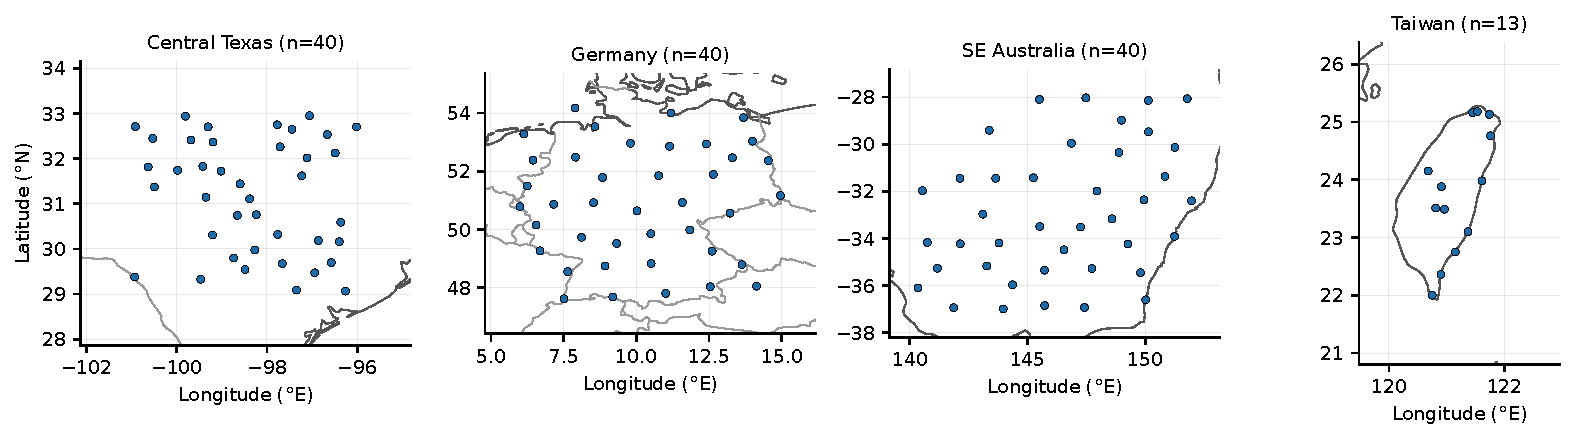
\includegraphics[width=\textwidth]{station_map.pdf}
\caption{Gauge stations used in the four regions (coastlines and borders: Natural Earth)}\label{fig:map}
\end{figure}

\subsection{Reference drought events}\label{sec:events}
Warning skill is scored against drought events defined from a quantity that no detector uses:
root-zone soil wetness from the MERRA-2 reanalysis \citep{gelaro2017}, extracted at each gauge from the
NASA POWER archive for 1981--2024. For each station, soil wetness is converted to a day-of-year
percentile, pooling a $\pm15$-day window over all years. Following run theory \citep{yevjevich1967}, an
event is a run of at least 30 consecutive days below the 20th percentile; runs separated by fewer than
30 days are merged, and an event is kept only if the preceding 60 days were not in drought. The onset is
the first day of the run. The target is therefore agricultural drought, defined independently of the
precipitation detectors and of the networks. The reference events include onsets in October 2010 in
central Texas, at the start of the driest 12-month period on record there \citep{hoerling2013}; in late
June 2018 in Germany, during the 2018--2019 central European drought \citep{hari2020}; in 2018 and 2019
in south-eastern Australia, during the 2017--2019 drought \citep{devanand2024}; and in October 2020 in
Taiwan, ahead of the spring 2021 drought \citep{chou2022} (Fig.~\ref{fig:traces}). Reanalysis soil moisture is itself a model product forced partly by
precipitation, and we return to this limitation in Section~\ref{sec:limits}.

\subsection{Study periods}
All networks and all climatological reference distributions are estimated on 1961--1990, the last
three years of which serve as an early-stopping validation set. Alarm thresholds are calibrated on
1991--2000. All warning and forecast results refer to 2001--2024, which no fitting step uses.

% ======================================================================
\section{Methods}\label{sec:methods}
\begin{figure}[t]
\centering
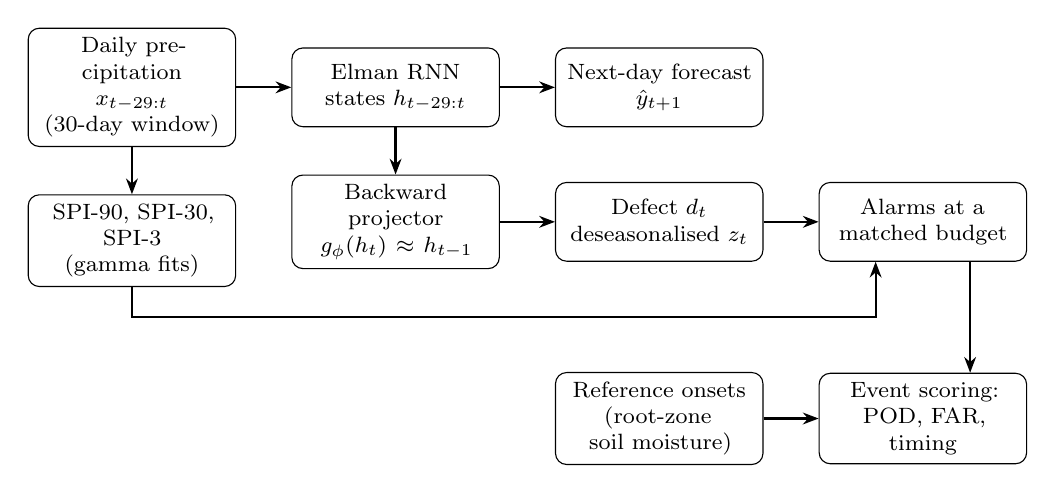
\begin{tikzpicture}[node distance=6mm and 7mm, every node/.style={font=\footnotesize},
 box/.style={draw,rounded corners,align=center,minimum height=10mm,text width=24mm},
 arr/.style={-{Stealth[length=2mm]},thick}]
 \node[box] (p) {Daily precipitation\\$x_{t-29:t}$\\(30-day window)};
 \node[box,right=of p] (h) {Elman RNN\\states $h_{t-29:t}$};
 \node[box,right=of h] (f) {Next-day forecast\\$\hat y_{t+1}$};
 \node[box,below=of p] (s) {SPI-90, SPI-30,\\SPI-3 (gamma fits)};
 \node[box,below=of h] (g) {Backward projector\\$g_\phi(h_t)\approx h_{t-1}$};
 \node[box,right=of g] (d) {Defect $d_t$\\deseasonalised $z_t$};
 \node[box,right=of d] (c) {Alarms at a\\matched budget};
 \node[box,below=14mm of d] (e) {Reference onsets\\(root-zone soil moisture)};
 \node[box,right=of e] (v) {Event scoring:\\POD, FAR, timing};
 \draw[arr] (p)--(h); \draw[arr] (h)--(f); \draw[arr] (h)--(g); \draw[arr] (g)--(d); \draw[arr] (d)--(c);
 \draw[arr] (p)--(s); \draw[arr] (e)--(v);
 \coordinate (cin) at ([xshift=-6mm]c.south); \coordinate (cout) at ([xshift=6mm]c.south);
 \coordinate (lvl) at ([yshift=-7mm]c.south);
 \draw[arr] (s.south) |- (cin |- lvl) -- (cin);
 \draw[arr] (cout) -- (cout |- v.north);
\end{tikzpicture}
\caption{Model, detectors and evaluation. Forecast accuracy and monitoring skill are evaluated
separately; reference events come from a variable that no detector uses}\label{fig:workflow}
\end{figure}

\subsection{Backward-coherence regularised recurrent network}\label{sec:model}
Let $x_t=(\tilde P_t,m_t)$, where $\tilde P_t$ is the standardised $\log(1+P_t)$ of daily precipitation
$P_t$ and $m_t$ indicates a missing observation; a missing day is filled with its 1961--1990
day-of-year climatology, so that missingness is never confused with zero rainfall. An Elman network with
$d=32$ hidden units maps a 30-day window $x_{t-29:t}$ to states $h_{t-29},\dots,h_t$ and to the
forecast $\hat y_{t+1}=w^\top h_t+b$ of $\tilde P_{t+1}$ (Fig.~\ref{fig:workflow}). A residual
multilayer perceptron $g_\phi(h)=h+W_2\,\mathrm{ReLU}(W_1h+b_1)+b_2$ reconstructs each state from its
successor, and the regularised objective over $n$ training windows is
\begin{equation}\label{eq:loss}
 \mathcal L(\theta,\phi)=\frac1n\sum_{t}\bigl(\hat y_{t+1}-\tilde P_{t+1}\bigr)^2
 +\frac{\lambda}{n}\sum_{t}\frac1{29}\sum_{s=t-29}^{t-1}\bigl\|h_s-g_\phi(h_{s+1})\bigr\|^2 .
\end{equation}

Let $\mathcal G_s=\sigma(h_u:u\ge s)$ be the decreasing filtration generated by the future of the
state path. A process with $\mathbb E[h_s\mid\mathcal G_{s+1}]=h_{s+1}$ is a reverse martingale
\citep{doob1953}. The projector $g_\phi(h_{s+1})$ is a one-step, first-order Markov surrogate for the
backward conditional expectation $\mathbb E[h_s\mid h_{s+1}]$, and the penalty in \eqref{eq:loss} is
its mean squared error. Minimising \eqref{eq:loss} does not make $(h_s)$ a reverse martingale; it makes
the representation approximately backward-predictable under the training climatology. This motivates
the monitoring statistic
\begin{equation}\label{eq:defect}
 d_t=\bigl\|h_{t-1}-g_\phi(h_t)\bigr\|,
\end{equation}
available once day $t$ has been observed. While the training regime persists, $\log d_t$ fluctuates
around a stable seasonal level; a persistent change in the input regime moves the state to a part of
the state space where the reconstruction error differs systematically. The direction of that shift is
empirical. In our exploratory work the defect fell during dry spells, which we attributed to a
near-constant input driving the state towards a near-stationary point that is easy to reconstruct; the
downward direction was therefore pre-specified. Whether a smoother state path improves monitoring is not assumed but
tested by the ablation below.

\paragraph{Training.} The penalty weight is $\lambda=0$ for three warm-up epochs and then decays
geometrically from 0.1 towards 0.01. We use Adam (learning rate $10^{-3}$, batch size 256, gradient
clipping at norm 1) for at most 40 epochs, with early stopping (patience 5) on the 1988--1990 validation
error, and with checkpoints eligible only once the penalty is active. Every configuration is trained
with five seeds per station.

\paragraph{Ablation and baseline.} The \emph{$\lambda=0$ ablation} has the identical backbone and
projector, but the projector is fitted on hidden states with stopped gradients. The defect
\eqref{eq:defect} is thus computed in exactly the same way, while the state path is not regularised.
A gated recurrent unit (GRU) network \citep{cho2014} of the same size is the forecasting baseline.

\subsection{Detectors}\label{sec:detectors}
All daily scores are converted to anomalies $z_t$ by subtracting a day-of-year mean and dividing by a
day-of-year standard deviation, both estimated on 1961--1990 and smoothed over $\pm15$ days;
seed-level anomalies are averaged over the five seeds. The pre-specified detectors are:
\begin{description}[leftmargin=1.2em,itemsep=2pt]
\item[D1, RM defect:] $z_t$ of $\log d_t$ from the regularised network.
\item[D2, ablation defect:] the same statistic from the $\lambda=0$ network.
\item[D3, daily SPI-90:] the 90-day precipitation total (at least 80 observed days, rescaled to 90)
transformed to a standard normal quantile through a zero-inflated gamma distribution fitted for each
day of year on 1961--1990 with $\pm15$-day pooling \citep{stagge2015}.
\item[D4, SPI-3:] the standard monthly index \citep{mckee1993,wmo2012}: monthly totals with at least
90\% observed days, three-month sums, and a zero-inflated gamma distribution for each calendar month on
1961--1990, updated once a month.
\item[D5, forecast residual:] $z_t$ of $\tilde P_t-\hat y_t$ from the regularised network, which asks
whether the defect carries information beyond the network's own forecast error.
\end{description}
Two detectors were added after the primary results had been seen and are reported as post hoc. D7 is a
daily SPI-30, built as D3 with a 30-day total (at least 27 observed days); it tests whether the
behaviour of the defect simply reflects the network's 30-day input window. D6 combines D1 and D3 by
monitoring the re-standardised mean of their anomalies.

D1, D2, D3, D5, D6 and D7 are monitored by the one-sided lower CUSUM \citep{page1954}
\begin{equation}\label{eq:cusum}
 C_t=\max\{0,\;C_{t-1}-z_t-k\},\qquad k=0.5,
\end{equation}
which alarms when $C_t\ge h$. Days with a missing score leave $C_t$ unchanged. After an alarm $C_t$ is
reset to zero and further alarms are suppressed for 90 days, so that one dry episode cannot produce a
burst of alarms. D4 alarms when SPI-3 first falls to or below a threshold $c$ (operationally $c=-1$),
with the same refractory period.

\subsection{Calibration at a matched alarm budget}\label{sec:calibration}
Nominal in-control average run lengths need not give comparable alarm rates here, because the scores
are autocorrelated and seasonally heteroscedastic and the calibration years contain droughts of their
own. We therefore
compare detectors at a matched \emph{alarm budget}. For each region and detector, the threshold $h$ (or
$c$) is chosen on a fine grid so that the detector raises, pooled over stations, $\beta$ alarms per
station-year during 1991--2000. The primary budget is $\beta=1$; $\beta=0.5$ and $\beta=2$ are
sensitivity analyses. Every detector then spends the same number of alarms, and differences on
2001--2024 reflect where the alarms fall rather than how many there are. Budgets that a detector cannot
attain (for example, a month-end rule cannot raise two alarms a year with a 90-day refractory period)
are flagged. We also report threshold-free operating curves of the probability of detection against the
false-alarm rate over the threshold grid on 2001--2024, analogous to the activity-monitoring operating
characteristic \citep{fawcett1999}.

\subsection{Event-based scoring and inference}\label{sec:scoring}
For each reference onset $\tau$ in 2001--2024, a detector scores a \emph{hit} if it alarms within
$[\tau-60,\tau+120]$ days, and its \emph{timing} is the first such alarm minus $\tau$ (negative values
are lead). An alarm outside $[\tau-60,\text{end}]$ of every event is a \emph{false alarm}. We report
the probability of detection (POD), the false-alarm rate (FAR, false alarms per station-year of
non-drought exposure) and the median timing of hits.

Stations in a region share weather, so station-events are not independent. Uncertainty is quantified
by a cluster bootstrap \citep{davison1997} that resamples the 24 calendar years within each region
(2000 replicates), preserving the cross-station dependence within a year; regions are resampled
independently. Differences between detectors are computed on the same replicates, giving paired
percentile intervals. Because conditional timing among hits depends on which events each detector
detects, timing is compared on events detected by both detectors.

\subsection{Physical association and incremental information}\label{sec:physical_methods}
To relate the defect to the hydrometeorological state, we regress station-month means of the D1 anomaly on SPI-3 and on MERRA-2 anomalies of
root-zone soil wetness, 2-m temperature and evapotranspiration (1981--2024), with station fixed effects
and standard errors clustered by year-month, which absorbs cross-station correlation. Predictors and
outcome are standardised. To ask whether the defect adds \emph{predictive} information, we fit weekly
logistic regressions for the event ``a reference drought begins within 60 days'', excluding weeks inside
an ongoing event, with SPI-90 alone or with the 30-day mean of D1, D2 or D5 added. Models are evaluated
by five-fold cross-validation over contiguous blocks of years; differences in AUC carry
region-year cluster-bootstrap intervals.

\subsection{Temperature-aware extension}\label{sec:mv_methods}
A network that sees precipitation alone can only summarise precipitation. To test whether a richer state
helps, we specified a second analysis in a protocol amendment, written after the results above were known
and before any temperature data were processed (Appendix~\ref{app:protocol}).

\paragraph{Temperature and evaporative demand.} Daily maximum and minimum temperature for 1961--2024 come
from the rain gauge itself when both series are at least 80\% complete in 1961--1990 and in 1991--2024,
and otherwise from the nearest GHCN-Daily station within 150~km that meets the same rule; for Taiwan they
are the synoptic stations' own records. Reference evapotranspiration $E_t$ is computed by the
Hargreaves--Samani formula \citep{hargreaves1985},
$E_t=0.0023\times0.408\,R_a\,(\bar T_t+17.8)\sqrt{T^{\max}_t-T^{\min}_t}$, with extraterrestrial radiation
$R_a$ from latitude and day of year \citep{allen1998}. Soil moisture is deliberately not an input, because
the reference events are defined from it.

\paragraph{Networks.} The input vector adds to $x_t$ the day-of-year anomalies of $T^{\max}_t$,
$T^{\min}_t$ and $E_t$ and a temperature-missingness indicator, and the network forecasts both next-day
precipitation and next-day $E_t$ with equal weight, so that its state must represent the thermal regime.
Architecture, penalty schedule, ablation, training rule and seeds are as in Section~\ref{sec:model}.

\paragraph{Detectors.} D8 and D9 are the defects of the temperature-aware network and of its $\lambda=0$
ablation. The natural comparators are now the standardised precipitation--evapotranspiration index
(SPEI; \citealp{vicenteserrano2010}) on daily 30- and 90-day sums of $P_t-E_t$ (D10 and D11), with a
three-parameter log-logistic distribution fitted for each day of year (pooling $\pm15$ days) on 1961--1990
by probability-weighted moments. D1, D3 and D7 are recomputed on the same stations. Calibration, scoring and
inference are exactly as in Sections~\ref{sec:calibration}--\ref{sec:scoring}, and the incremental-value
analysis uses SPEI-90, SPEI-30 and SPI-30 together as the base model.

\subsection{Forecast evaluation}\label{sec:forecast_methods}
Next-day forecasts of $\tilde P_{t+1}$ in 2001--2024 are scored by mean squared and absolute error, the
mean squared error skill score (MSESS) relative to day-of-year climatology, and the AUC for exceeding
the station's 1961--1990 95th percentile. Station-level paired differences between the regularised
network and the ablation or the GRU are tested with Wilcoxon signed-rank tests, and equivalence of
mean squared error with two one-sided tests (TOST) at a margin of $\pm2\%$ \citep{schuirmann1987}. The
path increment $Q_{\mathrm{path}}=\sum_s\|h_{s+1}-h_s\|$ over a window is compared within the Elman
backbone, where the hidden-state scale is comparable.

\subsection{Software}\label{sec:software}
All analyses were run in Python (PyTorch, NumPy, SciPy, statsmodels, scikit-learn and Numba); every
table and every number quoted in the text is generated directly from the result files by the published
code; the only exceptions are the pilot values in Appendix~\ref{app:protocol}, which are recorded in the
protocol's deviation log. AI tools were used to assist with code development and language editing; the authors checked all
code, analyses and results and take full responsibility for them.

% ======================================================================
\section{Results}\label{sec:results}
\subsection{Forecast accuracy and the state path}\label{sec:res_forecast}
Next-day precipitation is only weakly predictable from precipitation alone: MSESS against climatology
ranged from \msssmin\ to \msssmax\ across regions (Table~\ref{tab:forecast}). Within that limit the
regularisation was neutral (Table~\ref{tab:forecastpaired}). Pooled over \nstall\ stations, the 90\% confidence interval for the relative
MSE difference between the regularised network and its ablation was \msediffloall\% to \msediffhiall\%,
and against the GRU \msediffgruloall\% to \msediffgruhiall\%; equivalence within $\pm2\%$ was
established in every region (largest TOST $p$-value $\tostmax$). The regularisation reduced the
path increment by a median of \qpathred\% relative to the ablation (pooled Wilcoxon $p<10^{-4}$), with a
similar reduction in each region. The penalty therefore does what it is designed to do, smoothing the
state path, at no cost in forecast accuracy. Absolute $Q_{\mathrm{path}}$ values are not comparable
across architectures and the GRU values are shown only for completeness.

\begin{table}[t]
\caption{Next-day forecast accuracy on 2001--2024 (station means over five seeds, then averaged
over stations). MSE and MAE refer to standardised $\log(1+P)$; MSESS is the MSE skill score relative
to day-of-year climatology; AUC is for exceeding the station's 1961--1990 95th percentile;
$Q_{\mathrm{path}}$ is the mean hidden-state path increment over a 30-day window.}
\label{tab:forecast}
\footnotesize\setlength{\tabcolsep}{4pt}
\begin{tabular*}{\textwidth}{@{\extracolsep\fill}llrrrrr}
\toprule
Region & Model & MSE & MSESS & MAE & AUC & $Q_{\mathrm{path}}$\\
\midrule
Central Texas & RMRNN & 0.971 & 0.054 & 0.618 & 0.656 & 12.4 \\
 & $\lambda=0$ & 0.973 & 0.053 & 0.620 & 0.654 & 16.0 \\
 & GRU & 0.973 & 0.053 & 0.620 & 0.658 & 8.6 \\
\midrule
Germany & RMRNN & 0.916 & 0.103 & 0.758 & 0.671 & 17.6 \\
 & $\lambda=0$ & 0.917 & 0.103 & 0.759 & 0.671 & 23.0 \\
 & GRU & 0.916 & 0.103 & 0.758 & 0.671 & 13.2 \\
\midrule
SE Australia & RMRNN & 0.924 & 0.070 & 0.601 & 0.665 & 12.1 \\
 & $\lambda=0$ & 0.925 & 0.069 & 0.600 & 0.663 & 16.3 \\
 & GRU & 0.924 & 0.070 & 0.600 & 0.667 & 9.2 \\
\midrule
Taiwan & RMRNN & 0.782 & 0.176 & 0.670 & 0.806 & 16.6 \\
 & $\lambda=0$ & 0.782 & 0.176 & 0.670 & 0.805 & 21.2 \\
 & GRU & 0.780 & 0.178 & 0.668 & 0.806 & 13.7 \\
\midrule
All regions & RMRNN & 0.922 & 0.086 & 0.660 & 0.678 & 14.3 \\
 & $\lambda=0$ & 0.923 & 0.085 & 0.661 & 0.677 & 18.7 \\
 & GRU & 0.922 & 0.085 & 0.660 & 0.679 & 10.7 \\
\botrule
\end{tabular*}
\end{table}

\begin{table}[t]
\caption{Paired station-level comparisons of RMRNN. MSE differences are mean relative differences (\%)
with 90\% confidence intervals, which coincide with the TOST equivalence test at level 0.05: an interval
inside $\pm2\%$ establishes equivalence. $Q_{\mathrm{path}}$: median relative change (\%) against the
$\lambda=0$ ablation with its Wilcoxon signed-rank $p$-value.}
\label{tab:forecastpaired}
\footnotesize\setlength{\tabcolsep}{4pt}
\begin{tabular*}{\textwidth}{@{\extracolsep\fill}lrccrr}
\toprule
Region & $n$ & $\Delta$MSE vs $\lambda=0$ (\%) & $\Delta$MSE vs GRU (\%) & $\Delta Q_{\mathrm{path}}$ (\%) & $p$\\
\midrule
Central Texas & 40 & $-$0.13 [$-$0.22, $-$0.05] & $-$0.15 [$-$0.28, $-$0.02] & $-$22.1 & $<10^{-4}$ \\
Germany & 40 & $-$0.06 [$-$0.09, $-$0.02] & +0.03 [$-$0.04, +0.09] & $-$23.1 & $<10^{-4}$ \\
SE Australia & 40 & $-$0.04 [$-$0.11, +0.02] & +0.01 [$-$0.07, +0.08] & $-$26.3 & $<10^{-4}$ \\
Taiwan & 13 & $-$0.02 [$-$0.06, +0.02] & +0.25 [+0.07, +0.43] & $-$21.5 & 0.0002 \\
All regions & 133 & $-$0.07 [$-$0.11, $-$0.04] & $-$0.01 [$-$0.06, +0.04] & $-$23.5 & $<10^{-4}$ \\
\botrule
\end{tabular*}
\end{table}


\subsection{Warning skill at a matched alarm budget}\label{sec:res_warning}
Figure~\ref{fig:composites} shows the mean anomalies of the main statistics aligned on the reference
onsets. In Texas, Germany and Australia the defect declines in the weeks before onset and reaches its
minimum \compDonelaglo--\compDonelaghi\ days after onset, whereas SPI-90 reaches its minimum
\compDthreelaglo--\compDthreelaghi\ days after onset. SPI-30 falls further than the defect (composite
minima \compDsevenminlo\ to \compDsevenminhi, against \compDoneminlo\ to \compDoneminhi), with its
minimum \compDsevenlaglo--\compDsevenlaghi\ days after onset. In Taiwan the defect shows only a brief
dip at onset (\compDonemintaiwan) and is above zero again 30 days later (\compDonepostaiwan). The defect
and its ablation are almost indistinguishable throughout.

\begin{figure}[t]
\centering
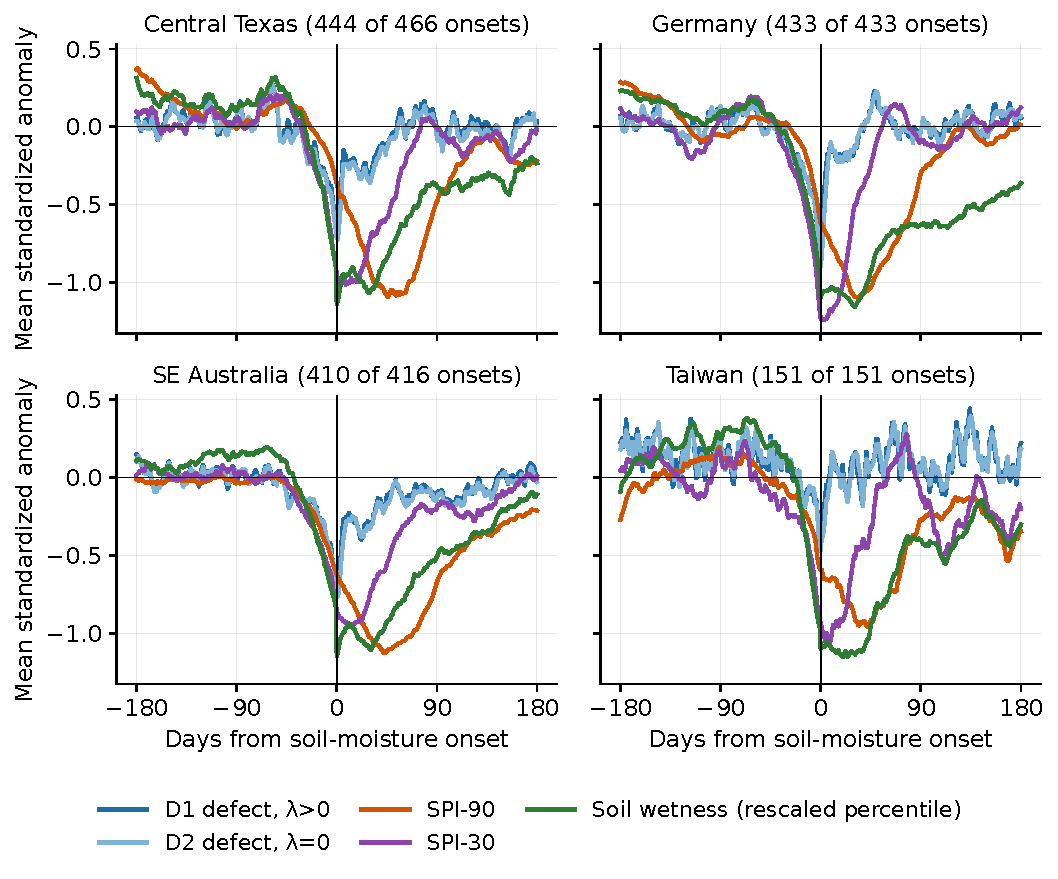
\includegraphics[width=\textwidth]{event_composites.pdf}
\caption{Mean daily anomalies aligned on reference soil-moisture onsets in 2001--2024 (day 0).
Soil wetness is shown as (percentile $-50)/28.9$, the standard deviation of a uniform percentile, so
that it shares the vertical scale}\label{fig:composites}
\end{figure}

Table~\ref{tab:warning} gives event-based skill at the primary budget of one alarm per station-year.
Pooled over regions, the defect detected \podallDone\ of the \nevall\ onsets, against \podallDthree\
for daily SPI-90, \podallDseven\ for daily SPI-30 and \podallDfour\ for monthly SPI-3; the forecast
residual detected \podallDfive, although its threshold grid could not match the budget within 10\% in
Texas, Germany and Australia (Table~\ref{tab:warning}). Pooled false-alarm rates were similar across the daily detectors, as
the matched budget intends, although in Germany the defect raised more false alarms than SPI-90
(Table~\ref{tab:paired}). Monthly SPI-3 performed poorly in Germany and Australia; a likely reason, which
we did not test, is that month-end updates combined with the 90-day refractory period miss onsets that
fall between decisions. For a daily monitor, daily SPI-90 is the more relevant benchmark.

\begin{table}[t]
\caption{Event-based warning skill on 2001--2024 at a matched budget of 1 alarm(s) per
station-year (calibrated on 1991--2000). POD: probability of detection within $[-60,+120]$ days of a
reference onset; FAR: false alarms per station-year of non-drought exposure; timing: median of
(alarm $-$ onset) among hits, negative values meaning lead. Brackets: 95\% cluster-bootstrap intervals
(calendar years resampled within region). $^{\dagger}$Post hoc (not pre-specified).
$^{\ast}$Budget not attained within 10\% in calibration (closest attainable rate used).}
\label{tab:warning}
\footnotesize\setlength{\tabcolsep}{4pt}
\begin{tabular*}{\textwidth}{@{\extracolsep\fill}lccc}
\toprule
Detector & POD & FAR (per yr) & Median timing (d)\\
\midrule
\multicolumn{4}{l}{\textit{Central Texas} (466 events)}\\
\quad D1 RM defect & 0.71 [0.62, 0.79] & 0.93 [0.80, 1.07] & +16 [+6, +21] \\
\quad D2 defect, $\lambda=0$ & 0.69 [0.61, 0.77] & 0.94 [0.81, 1.08] & +15 [+6, +23] \\
\quad D3 SPI-90 (daily) & 0.81 [0.74, 0.87] & 0.85 [0.69, 1.04] & +30 [+26, +35] \\
\quad D4 SPI-3 (monthly) & 0.81 [0.75, 0.87] & 0.93 [0.79, 1.07] & +25 [+19, +31] \\
\quad D5 forecast residual$^{\ast}$ & 0.36 [0.28, 0.45] & 1.22 [1.09, 1.33] & +47 [+30, +55] \\
\quad D7 SPI-30 (daily)$^{\dagger}$ & 0.79 [0.72, 0.86] & 0.93 [0.78, 1.11] & +14 [+9, +17] \\
\quad D6 D1+D3 combined$^{\dagger}$ & 0.79 [0.71, 0.86] & 0.88 [0.71, 1.08] & +23 [+18, +29] \\
\midrule
\multicolumn{4}{l}{\textit{Germany} (433 events)}\\
\quad D1 RM defect & 0.63 [0.54, 0.71] & 0.84 [0.71, 0.99] & +0 [$-$4, +6] \\
\quad D2 defect, $\lambda=0$ & 0.62 [0.53, 0.71] & 0.83 [0.69, 1.00] & +1 [$-$4, +7] \\
\quad D3 SPI-90 (daily) & 0.74 [0.63, 0.83] & 0.66 [0.51, 0.82] & +26 [+10, +35] \\
\quad D4 SPI-3 (monthly) & 0.35 [0.27, 0.44] & 1.18 [1.03, 1.33] & $-$1 [$-$13, +8] \\
\quad D5 forecast residual$^{\ast}$ & 0.41 [0.35, 0.49] & 1.24 [1.14, 1.36] & +34 [+23, +39] \\
\quad D7 SPI-30 (daily)$^{\dagger}$ & 0.75 [0.65, 0.84] & 0.72 [0.57, 0.92] & +9 [+5, +14] \\
\quad D6 D1+D3 combined$^{\dagger}$ & 0.73 [0.62, 0.81] & 0.70 [0.56, 0.85] & +17 [+5, +29] \\
\midrule
\multicolumn{4}{l}{\textit{SE Australia} (416 events)}\\
\quad D1 RM defect & 0.71 [0.64, 0.77] & 0.83 [0.73, 0.94] & +12 [+3, +23] \\
\quad D2 defect, $\lambda=0$ & 0.73 [0.66, 0.79] & 0.87 [0.77, 0.99] & +12 [+2, +25] \\
\quad D3 SPI-90 (daily) & 0.81 [0.76, 0.86] & 0.85 [0.67, 1.03] & +22 [+16, +29] \\
\quad D4 SPI-3 (monthly) & 0.32 [0.26, 0.40] & 0.93 [0.82, 1.04] & $-$6 [$-$20, +8] \\
\quad D5 forecast residual$^{\ast}$ & 0.22 [0.18, 0.27] & 0.70 [0.62, 0.76] & +63 [+56, +71] \\
\quad D7 SPI-30 (daily)$^{\dagger}$ & 0.76 [0.70, 0.80] & 0.76 [0.62, 0.90] & +18 [+11, +26] \\
\quad D6 D1+D3 combined$^{\dagger}$ & 0.85 [0.80, 0.90] & 0.87 [0.68, 1.07] & +16 [+9, +24] \\
\midrule
\multicolumn{4}{l}{\textit{Taiwan} (151 events)}\\
\quad D1 RM defect & 0.50 [0.37, 0.60] & 0.61 [0.47, 0.75] & +7 [$-$5, +22] \\
\quad D2 defect, $\lambda=0$ & 0.45 [0.33, 0.56] & 0.67 [0.54, 0.81] & +10 [$-$4, +27] \\
\quad D3 SPI-90 (daily) & 0.55 [0.44, 0.64] & 0.70 [0.47, 0.93] & +33 [+19, +48] \\
\quad D4 SPI-3 (monthly) & 0.56 [0.45, 0.66] & 0.82 [0.62, 1.01] & +30 [+16, +46] \\
\quad D5 forecast residual & 0.42 [0.33, 0.52] & 1.02 [0.89, 1.15] & +24 [+4, +35] \\
\quad D7 SPI-30 (daily)$^{\dagger}$ & 0.52 [0.40, 0.63] & 0.70 [0.53, 0.88] & +17 [+13, +28] \\
\quad D6 D1+D3 combined$^{\dagger}$ & 0.54 [0.40, 0.65] & 0.60 [0.39, 0.84] & +29 [+12, +38] \\
\midrule
\multicolumn{4}{l}{\textit{All regions} (1466 events)}\\
\quad D1 RM defect & 0.67 [0.62, 0.71] & 0.84 [0.78, 0.91] & +8 [+4, +14] \\
\quad D2 defect, $\lambda=0$ & 0.65 [0.61, 0.70] & 0.86 [0.80, 0.94] & +9 [+5, +15] \\
\quad D3 SPI-90 (daily) & 0.76 [0.72, 0.80] & 0.78 [0.69, 0.87] & +27 [+23, +31] \\
\quad D4 SPI-3 (monthly) & 0.51 [0.46, 0.56] & 0.99 [0.92, 1.07] & +14 [+9, +20] \\
\quad D5 forecast residual & 0.34 [0.30, 0.38] & 1.04 [0.99, 1.10] & +43 [+35, +48] \\
\quad D7 SPI-30 (daily)$^{\dagger}$ & 0.74 [0.70, 0.78] & 0.79 [0.72, 0.88] & +13 [+10, +16] \\
\quad D6 D1+D3 combined$^{\dagger}$ & 0.76 [0.72, 0.80] & 0.80 [0.71, 0.89] & +20 [+15, +24] \\
\botrule
\end{tabular*}
\end{table}


The paired comparisons (Table~\ref{tab:paired}) separate three questions. \emph{Does the defect beat
standard indices?} Against daily SPI-90 the defect detected fewer onsets in every region (with
intervals excluding zero in all but Taiwan), by
\dpodallDoneDthree\ pooled (95\% CI \dpodloallDoneDthree\ to \dpodhiallDoneDthree), at a similar
false-alarm rate. On the events both detected, however, the defect alarmed a median of
\dtimallDoneDthree\ days earlier (CI \dtimloallDoneDthree\ to \dtimhiallDoneDthree), and earlier in
\fearlyallDoneDthree\% of them. The defect is thus faster but less sensitive. Pooled over regions it
detected more onsets than monthly SPI-3 (\dpodallDoneDfour) with fewer false alarms, but not in every
region: in Texas SPI-3 detected more onsets, and in Taiwan the difference was not significant. \emph{Does the regularisation
matter for monitoring?} No: the defect of the regularised network and of its ablation differed by
\dpodallDoneDtwo\ in POD (CI \dpodloallDoneDtwo\ to \dpodhiallDoneDtwo) and by a median of
\dtimallDoneDtwo\ days in timing. \emph{Is the defect's speed a matter of time scale?} Largely yes. SPI-30
was nearly as sensitive as SPI-90 (difference \dpodallDsevenDthree, CI \dpodloallDsevenDthree\ to
\dpodhiallDsevenDthree) and alarmed \dtimallDsevenDthree\ days earlier than SPI-90, which accounts for
most of the defect's \dtimallDoneDthree-day advantage (the two timing comparisons are made on different
sets of jointly detected events); the defect remained \dtimallDoneDseven\ days
(CI \dtimloallDoneDseven\ to \dtimhiallDoneDseven) faster than SPI-30 but detected fewer onsets
(\dpodallDoneDseven, CI \dpodloallDoneDseven\ to \dpodhiallDoneDseven).

\begin{table}[t]
\caption{Paired comparisons at the primary budget (1 alarm per station-year). $\Delta$POD and
$\Delta$FAR are first minus second detector; $\Delta$timing is the median, over events detected by both,
of (second detector's alarm $-$ first detector's alarm), so positive values mean the first detector
alarms earlier. Brackets: 95\% cluster-bootstrap intervals. $^{\dagger}$Post hoc.}
\label{tab:paired}
\footnotesize\setlength{\tabcolsep}{4pt}
\begin{tabular*}{\textwidth}{@{\extracolsep\fill}lcccr}
\toprule
Comparison & $\Delta$POD & $\Delta$FAR (per yr) & $\Delta$timing (d) & $n$ both\\
\midrule
\multicolumn{5}{l}{\textit{Central Texas}}\\
\quad D1 vs D2 ($\lambda=0$) & +0.021 [$-$0.018, +0.054] & $-$0.01 [$-$0.04, +0.02] & +0.0 [$-$1.0, +0.0] & 294 \\
\quad D1 vs D3 (SPI-90) & $-$0.101 [$-$0.188, $-$0.024] & +0.08 [$-$0.07, +0.23] & +16.0 [+8.5, +23.0] & 294 \\
\quad D1 vs D4 (SPI-3) & $-$0.101 [$-$0.172, $-$0.034] & +0.00 [$-$0.16, +0.18] & +9.0 [+3.0, +15.0] & 288 \\
\quad D1 vs D7 (SPI-30)$^{\dagger}$ & $-$0.086 [$-$0.165, $-$0.014] & $-$0.00 [$-$0.10, +0.09] & +3.0 [+0.0, +5.0] & 298 \\
\quad D7 vs D3$^{\dagger}$ & $-$0.015 [$-$0.051, +0.023] & +0.08 [$-$0.04, +0.20] & +18.0 [+16.0, +23.0] & 340 \\
\quad D6 vs D3$^{\dagger}$ & $-$0.019 [$-$0.057, +0.019] & +0.02 [$-$0.02, +0.07] & +4.0 [+3.0, +5.0] & 349 \\
\midrule
\multicolumn{5}{l}{\textit{Germany}}\\
\quad D1 vs D2 ($\lambda=0$) & +0.014 [$-$0.013, +0.042] & +0.00 [$-$0.05, +0.05] & +1.0 [+0.0, +1.0] & 245 \\
\quad D1 vs D3 (SPI-90) & $-$0.106 [$-$0.188, $-$0.019] & +0.18 [+0.02, +0.34] & +21.5 [+8.0, +37.0] & 226 \\
\quad D1 vs D4 (SPI-3) & +0.284 [+0.140, +0.411] & $-$0.35 [$-$0.53, $-$0.17] & +2.0 [$-$16.0, +14.0] & 92 \\
\quad D1 vs D7 (SPI-30)$^{\dagger}$ & $-$0.120 [$-$0.171, $-$0.069] & +0.11 [+0.00, +0.23] & +7.0 [+3.0, +10.0] & 239 \\
\quad D7 vs D3$^{\dagger}$ & +0.014 [$-$0.056, +0.088] & +0.07 [$-$0.05, +0.18] & +15.5 [+6.0, +25.0] & 284 \\
\quad D6 vs D3$^{\dagger}$ & $-$0.012 [$-$0.036, +0.011] & +0.04 [$-$0.01, +0.08] & +5.0 [+3.0, +7.0] & 303 \\
\midrule
\multicolumn{5}{l}{\textit{SE Australia}}\\
\quad D1 vs D2 ($\lambda=0$) & $-$0.019 [$-$0.056, +0.020] & $-$0.04 [$-$0.08, +0.00] & +0.0 [$-$0.5, +1.0] & 273 \\
\quad D1 vs D3 (SPI-90) & $-$0.101 [$-$0.171, $-$0.036] & $-$0.01 [$-$0.11, +0.09] & +11.5 [+3.0, +16.0] & 256 \\
\quad D1 vs D4 (SPI-3) & +0.387 [+0.270, +0.485] & $-$0.10 [$-$0.27, +0.09] & $-$28.0 [$-$37.5, $-$7.0] & 90 \\
\quad D1 vs D7 (SPI-30)$^{\dagger}$ & $-$0.048 [$-$0.097, $-$0.002] & +0.08 [+0.01, +0.14] & +7.0 [+5.0, +10.0] & 259 \\
\quad D7 vs D3$^{\dagger}$ & $-$0.053 [$-$0.092, $-$0.017] & $-$0.09 [$-$0.18, $-$0.00] & +8.0 [+4.0, +13.0] & 288 \\
\quad D6 vs D3$^{\dagger}$ & +0.038 [+0.010, +0.066] & +0.03 [$-$0.01, +0.06] & +6.0 [+4.0, +7.0] & 330 \\
\midrule
\multicolumn{5}{l}{\textit{Taiwan}}\\
\quad D1 vs D2 ($\lambda=0$) & +0.046 [$-$0.013, +0.115] & $-$0.06 [$-$0.12, +0.01] & +1.0 [+0.0, +2.0] & 60 \\
\quad D1 vs D3 (SPI-90) & $-$0.053 [$-$0.185, +0.078] & $-$0.09 [$-$0.30, +0.14] & +30.0 [+11.0, +41.0] & 49 \\
\quad D1 vs D4 (SPI-3) & $-$0.060 [$-$0.153, +0.018] & $-$0.21 [$-$0.41, $-$0.03] & +17.0 [$-$9.0, +45.0] & 51 \\
\quad D1 vs D7 (SPI-30)$^{\dagger}$ & $-$0.026 [$-$0.127, +0.070] & $-$0.09 [$-$0.24, +0.06] & +17.0 [+6.0, +23.0] & 52 \\
\quad D7 vs D3$^{\dagger}$ & $-$0.026 [$-$0.110, +0.067] & +0.00 [$-$0.13, +0.14] & +13.5 [$-$0.5, +22.0] & 64 \\
\quad D6 vs D3$^{\dagger}$ & $-$0.007 [$-$0.064, +0.047] & $-$0.10 [$-$0.16, $-$0.04] & +1.0 [$-$2.0, +5.0] & 74 \\
\midrule
\multicolumn{5}{l}{\textit{All regions}}\\
\quad D1 vs D2 ($\lambda=0$) & +0.010 [$-$0.009, +0.029] & $-$0.02 [$-$0.04, +0.00] & +0.0 [+0.0, +0.0] & 872 \\
\quad D1 vs D3 (SPI-90) & $-$0.098 [$-$0.140, $-$0.056] & +0.06 [$-$0.01, +0.14] & +16.0 [+12.0, +22.0] & 825 \\
\quad D1 vs D4 (SPI-3) & +0.156 [+0.086, +0.225] & $-$0.15 [$-$0.25, $-$0.05] & +5.0 [$-$3.0, +10.5] & 521 \\
\quad D1 vs D7 (SPI-30)$^{\dagger}$ & $-$0.079 [$-$0.112, $-$0.046] & +0.05 [$-$0.01, +0.09] & +6.0 [+4.0, +7.0] & 848 \\
\quad D7 vs D3$^{\dagger}$ & $-$0.018 [$-$0.045, +0.010] & +0.01 [$-$0.04, +0.07] & +15.0 [+12.0, +17.0] & 976 \\
\quad D6 vs D3$^{\dagger}$ & +0.001 [$-$0.017, +0.018] & +0.02 [$-$0.01, +0.04] & +5.0 [+4.0, +6.0] & 1056 \\
\botrule
\end{tabular*}
\end{table}


The operating curves (Fig.~\ref{fig:amoc}) show the same ordering over a range of thresholds: at
false-alarm rates from 0.5 to 2 per station-year the SPI-90 and SPI-30 curves lie on or above the
defect curve in every region, and the curves of the defect and its ablation differ by at most
\amocDoneDtwomaxdiff\ in POD. At budgets of 0.5 and 2 alarms per station-year (Online Resource 1,
Tables~\ref{S-tab:warning05}--\ref{S-tab:warning2}) the pooled comparisons with SPI-90, SPI-30 and the
ablation lead to the same conclusions.

\begin{figure}[t]
\centering
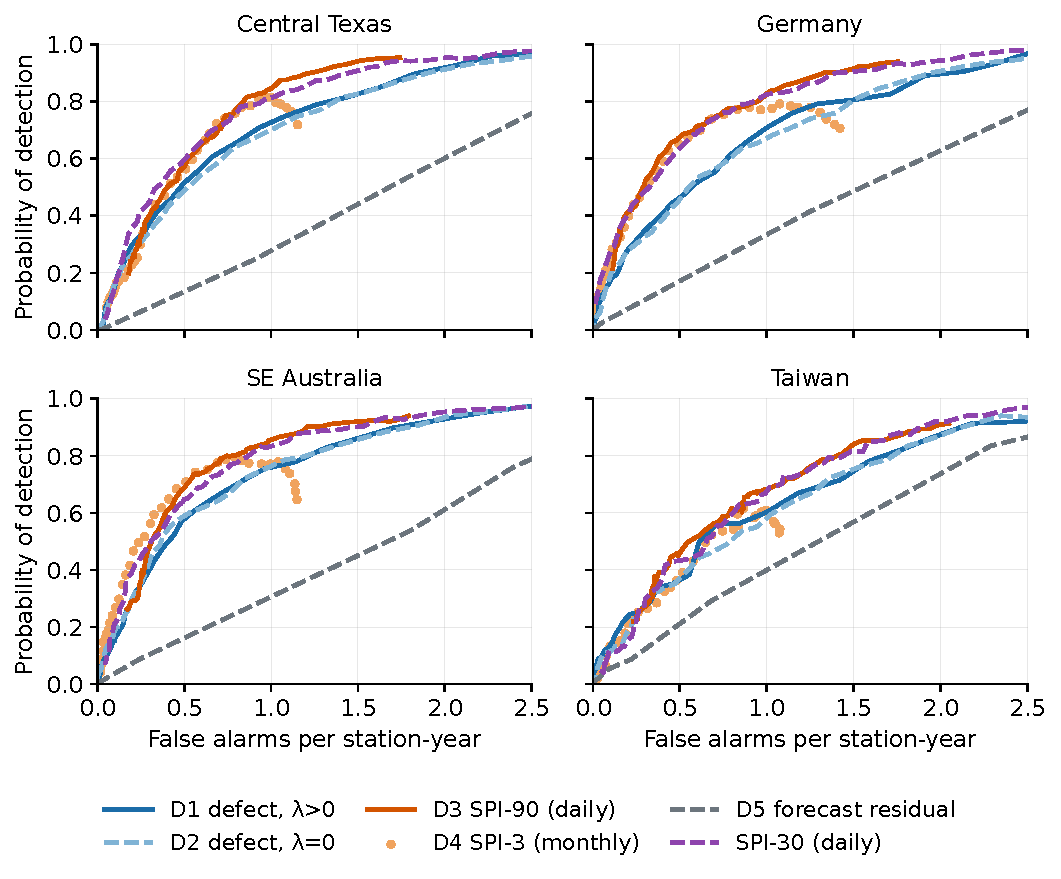
\includegraphics[width=\textwidth]{operating_curves.pdf}
\caption{Threshold-free operating curves on 2001--2024: probability of detection against false alarms
per station-year as the threshold varies. SPI-3 is a month-end threshold rule whose alarm count is not
monotone in the threshold and is shown as points}\label{fig:amoc}
\end{figure}

The post hoc combination D6 detected as many onsets as SPI-90 (difference \dpodallDsixDthree, CI
\dpodloallDsixDthree\ to \dpodhiallDsixDthree) and alarmed \dtimallDsixDthree\ days earlier on events
both detected (CI \dtimloallDsixDthree\ to \dtimhiallDsixDthree), with a false-alarm difference of
\dfarallDsixDthree\ per year. The timing gain was significant in Texas, Germany and Australia but not
in Taiwan. It is a small gain from adding a short-memory component to SPI-90, comparable to what SPI-30
provides.

Figure~\ref{fig:traces} shows the droughts cited in Section~\ref{sec:events} at one station each,
chosen for illustration rather than as a test. In the Texas, German and Australian cases the defect
alarmed \traceDonelaglo--\traceDonelaghi\ days after the reference onset and
\traceDthreeminusDonelo--\traceDthreeminusDonehi\ days before SPI-90, and SPI-30 alarmed
\traceDsevenminusDonelo--\traceDsevenminusDonehi\ days after the defect. In the Taiwan case the defect
did not alarm, whereas SPI-30 alarmed \traceDseventaiwan\ day before the onset and SPI-90
\traceDthreetaiwan\ days after it.

\begin{figure}[p]
\centering
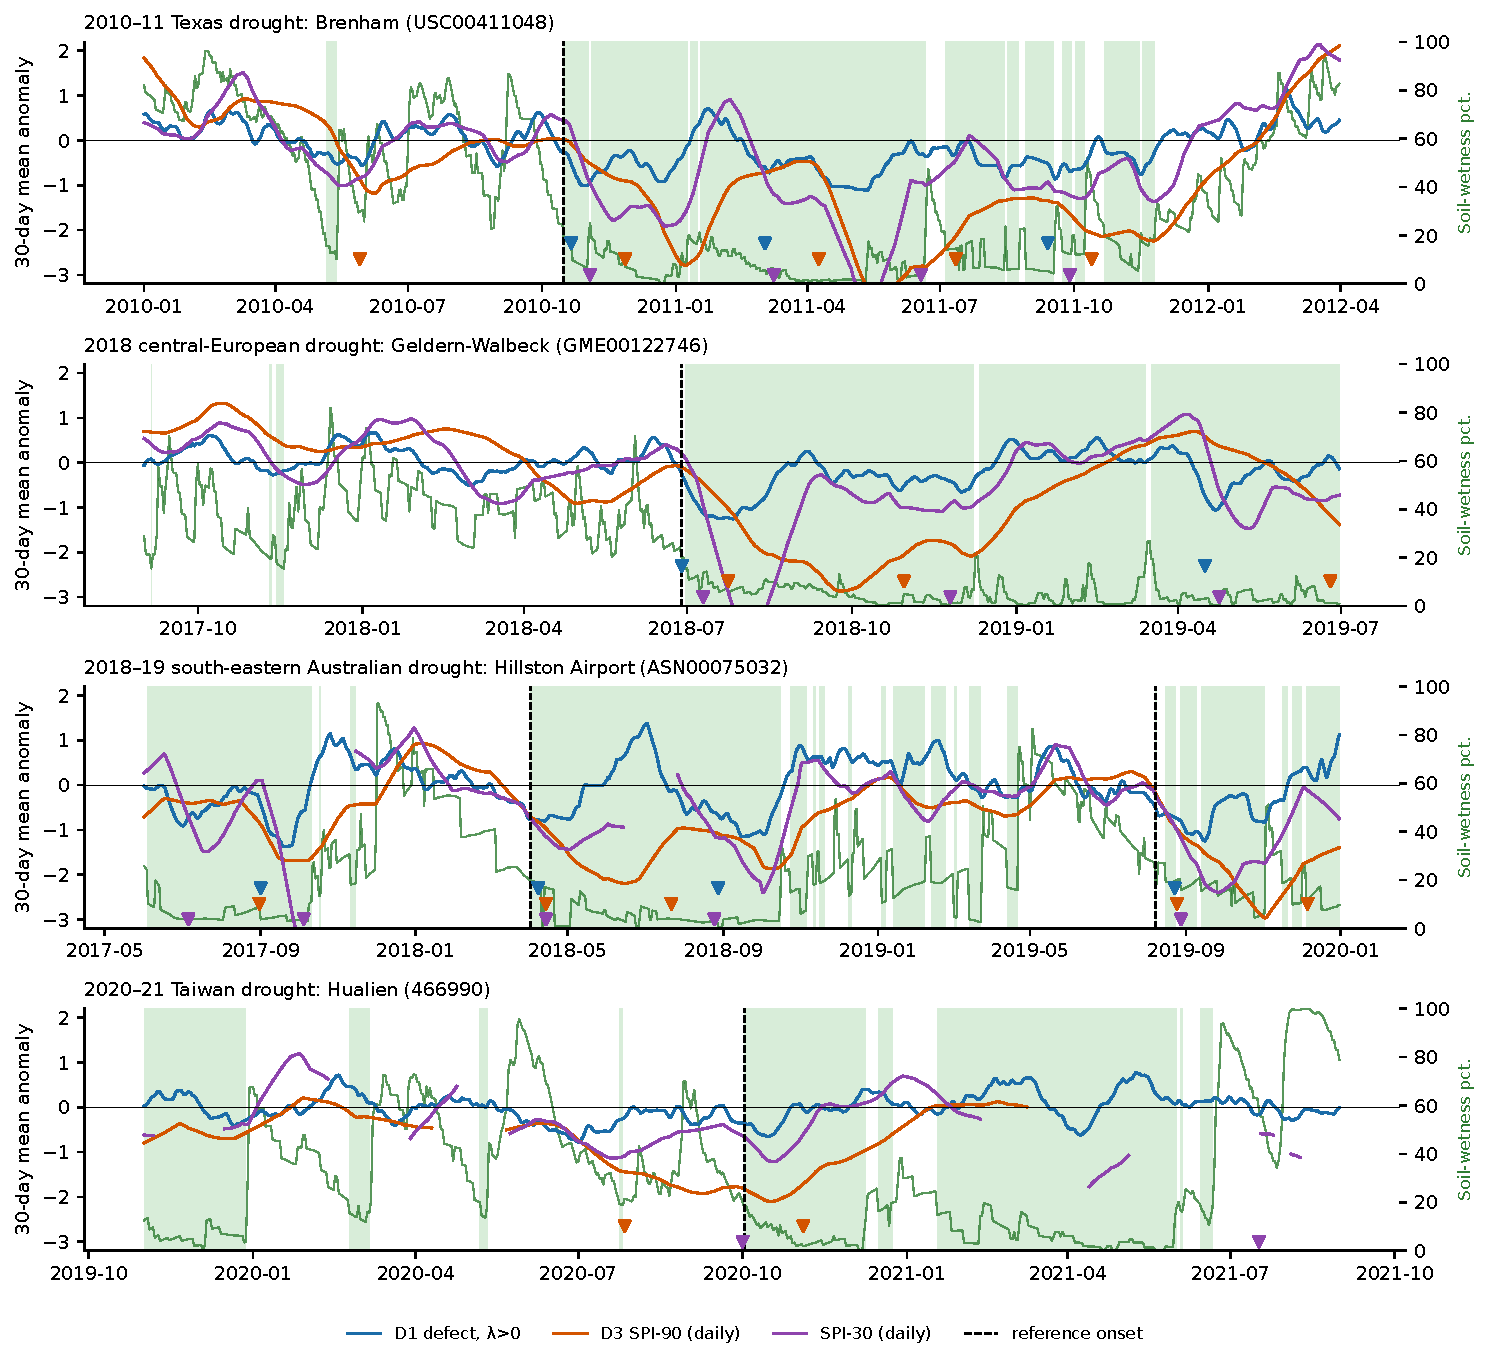
\includegraphics[width=\textwidth]{event_traces.pdf}
\caption{Four droughts at illustrative stations. Lines: 30-day running means of the
daily anomalies of the defect (D1), SPI-90 and SPI-30; triangles: alarms of each detector at the
primary budget; shading: root-zone soil wetness below the 20th percentile (right axis: percentile);
dashed lines: reference onsets. Gaps in SPI-30 are days with fewer than 27 observed days in the
window}\label{fig:traces}
\end{figure}

\subsection{What the defect measures}\label{sec:physical}
The defect anomaly rose and fell with SPI-3 in every region, and in Texas, Australia and Taiwan it was
also associated with root-zone soil moisture after adjusting for SPI-3, temperature and
evapotranspiration (Table~\ref{tab:assoc}, Fig.~\ref{fig:assoc}). It was negatively associated with
evapotranspiration in Germany, Australia and Taiwan. These anomalies explain between a fifth and more
than a third of the within-station variation of the monthly defect ($R^2_w$ in Table~\ref{tab:assoc}).
Its ablation has nearly identical coefficients, so the association does not depend on the
regularisation. Because the network sees precipitation only, the soil-moisture association beyond SPI-3
may reflect the sub-seasonal timing of rainfall within the three-month window, to which a 30-day
recurrent summary is sensitive and SPI-3 is not. We did not test this explanation, and we do not
interpret the association as evidence that the network infers land-surface processes.

\begin{table}[tbp]
\caption{Monthly association (1981--2024) between the defect anomaly and concurrent
hydrometeorological anomalies: standardised coefficients from regressions with station fixed effects;
$^{\ast}p<0.05$ with standard errors clustered by year-month; $R^2_w$ is the within-station $R^2$.}
\label{tab:assoc}
\footnotesize\setlength{\tabcolsep}{4pt}
\begin{tabular*}{\textwidth}{@{\extracolsep\fill}lrrrrrrrrrr}
\toprule
& \multicolumn{5}{c}{D1 defect, $\lambda>0$} & \multicolumn{5}{c}{D2 defect, $\lambda=0$}\\
\cmidrule{2-6}\cmidrule{7-11}
Region & SPI-3 & SM & T2m & ET & $R^2_w$ & SPI-3 & SM & T2m & ET & $R^2_w$\\
\midrule
Central Texas & +0.28$^{\ast}$ & +0.32$^{\ast}$ & $-$0.16$^{\ast}$ & $-$0.06 & 0.36 & +0.26$^{\ast}$ & +0.30$^{\ast}$ & $-$0.18$^{\ast}$ & $-$0.06 & 0.34 \\
Germany & +0.53$^{\ast}$ & $-$0.01 & +0.03 & $-$0.15$^{\ast}$ & 0.30 & +0.48$^{\ast}$ & +0.00 & +0.04 & $-$0.15$^{\ast}$ & 0.25 \\
SE Australia & +0.41$^{\ast}$ & +0.44$^{\ast}$ & +0.01 & $-$0.24$^{\ast}$ & 0.37 & +0.40$^{\ast}$ & +0.42$^{\ast}$ & $-$0.00 & $-$0.23$^{\ast}$ & 0.34 \\
Taiwan & +0.29$^{\ast}$ & +0.25$^{\ast}$ & +0.06$^{\ast}$ & $-$0.18$^{\ast}$ & 0.20 & +0.26$^{\ast}$ & +0.24$^{\ast}$ & +0.07$^{\ast}$ & $-$0.14$^{\ast}$ & 0.18 \\
All regions & +0.43$^{\ast}$ & +0.14$^{\ast}$ & $-$0.06$^{\ast}$ & $-$0.02 & 0.30 & +0.40$^{\ast}$ & +0.14$^{\ast}$ & $-$0.06$^{\ast}$ & $-$0.02 & 0.27 \\
\botrule
\end{tabular*}
\end{table}


\begin{figure}[t]
\centering
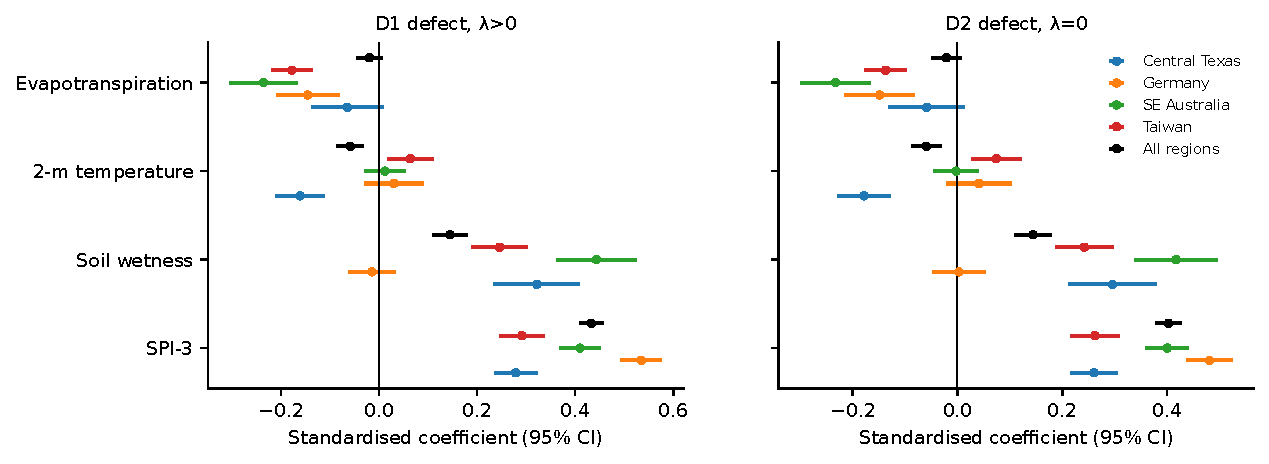
\includegraphics[width=0.9\textwidth]{association.pdf}
\caption{Standardised coefficients (95\% CIs) of concurrent hydrometeorological anomalies in monthly
regressions of the defect anomaly, by region}\label{fig:assoc}
\end{figure}

Predicting onset within 60 days was hard for every precipitation statistic we tested: the cross-validated AUC of
SPI-90 alone ranged from \aucbasetaiwan\ in Taiwan, below the chance level of 0.5, to \aucbaseaustralia\
in Australia (Table~\ref{tab:incremental}). Adding the 30-day mean defect raised the pooled AUC
by \daucallDone\ (CI \daucloallDone\ to \dauchiallDone), and the ablation defect by a similar
amount. Adding SPI-30 instead raised it by \daucallSPIthirty, and once SPI-30 was included the defect
added nothing (\daucallSPIthirtypDone, CI \daucloallSPIthirtypDone\ to \dauchiallSPIthirtypDone), in
every region. The 30-day mean forecast residual, itself a short-window precipitation anomaly, added
\daucallDfive. The defect thus carries statistically detectable information about impending onset, but
in these data that information is contained in a 30-day precipitation summary.

\begin{table}[t]
\caption{Incremental information about drought onset within 60 days (weekly logistic models,
five-fold cross-validation over blocks of years, 1982--2024). $\Delta$AUC is relative to the reference
model; brackets are 95\% region-year cluster-bootstrap intervals. Predictors other than SPI are
30-day means. $^{\dagger}$Post hoc.}
\label{tab:incremental}
\footnotesize\setlength{\tabcolsep}{4pt}
\begin{tabular*}{\textwidth}{@{\extracolsep\fill}llcc}
\toprule
Model & Reference & AUC & $\Delta$AUC\\
\midrule
\multicolumn{4}{l}{\textit{Central Texas} (base AUC 0.544, prevalence 0.083)}\\
\quad SPI-90 + D1 & SPI-90 & 0.576 & +0.033 [+0.010, +0.057] \\
\quad SPI-90 + D2 & SPI-90 & 0.574 & +0.030 [+0.007, +0.054] \\
\quad SPI-90 + D5 & SPI-90 & 0.597 & +0.053 [+0.029, +0.079] \\
\quad SPI-90 + SPI-30$^{\dagger}$ & SPI-90 & 0.586 & +0.043 [+0.022, +0.065] \\
\quad SPI-90 + SPI-30 + D1$^{\dagger}$ & SPI-90 + SPI-30 & 0.585 & $-$0.002 [$-$0.007, +0.003] \\
\midrule
\multicolumn{4}{l}{\textit{Germany} (base AUC 0.561, prevalence 0.085)}\\
\quad SPI-90 + D1 & SPI-90 & 0.574 & +0.012 [+0.004, +0.021] \\
\quad SPI-90 + D2 & SPI-90 & 0.571 & +0.010 [+0.001, +0.018] \\
\quad SPI-90 + D5 & SPI-90 & 0.599 & +0.037 [+0.023, +0.050] \\
\quad SPI-90 + SPI-30$^{\dagger}$ & SPI-90 & 0.591 & +0.029 [+0.017, +0.041] \\
\quad SPI-90 + SPI-30 + D1$^{\dagger}$ & SPI-90 + SPI-30 & 0.590 & $-$0.0009 [$-$0.0042, +0.0023] \\
\midrule
\multicolumn{4}{l}{\textit{SE Australia} (base AUC 0.589, prevalence 0.073)}\\
\quad SPI-90 + D1 & SPI-90 & 0.612 & +0.022 [+0.009, +0.038] \\
\quad SPI-90 + D2 & SPI-90 & 0.608 & +0.019 [+0.005, +0.034] \\
\quad SPI-90 + D5 & SPI-90 & 0.632 & +0.043 [+0.025, +0.063] \\
\quad SPI-90 + SPI-30$^{\dagger}$ & SPI-90 & 0.626 & +0.037 [+0.020, +0.056] \\
\quad SPI-90 + SPI-30 + D1$^{\dagger}$ & SPI-90 + SPI-30 & 0.626 & $-$0.0001 [$-$0.0017, +0.0013] \\
\midrule
\multicolumn{4}{l}{\textit{Taiwan} (base AUC 0.434, prevalence 0.097)}\\
\quad SPI-90 + D1 & SPI-90 & 0.480 & +0.045 [+0.017, +0.070] \\
\quad SPI-90 + D2 & SPI-90 & 0.459 & +0.025 [+0.005, +0.045] \\
\quad SPI-90 + D5 & SPI-90 & 0.554 & +0.120 [+0.075, +0.159] \\
\quad SPI-90 + SPI-30$^{\dagger}$ & SPI-90 & 0.529 & +0.095 [+0.052, +0.134] \\
\quad SPI-90 + SPI-30 + D1$^{\dagger}$ & SPI-90 + SPI-30 & 0.526 & $-$0.003 [$-$0.008, +0.001] \\
\midrule
\multicolumn{4}{l}{\textit{All regions} (base AUC 0.575, prevalence 0.082)}\\
\quad SPI-90 + D1 & SPI-90 & 0.597 & +0.022 [+0.014, +0.030] \\
\quad SPI-90 + D2 & SPI-90 & 0.594 & +0.019 [+0.011, +0.026] \\
\quad SPI-90 + D5 & SPI-90 & 0.618 & +0.043 [+0.032, +0.055] \\
\quad SPI-90 + SPI-30$^{\dagger}$ & SPI-90 & 0.611 & +0.036 [+0.026, +0.045] \\
\quad SPI-90 + SPI-30 + D1$^{\dagger}$ & SPI-90 + SPI-30 & 0.610 & $-$0.0004 [$-$0.0012, +0.0002] \\
\botrule
\end{tabular*}
\end{table}


\subsection{Temperature-aware networks}\label{sec:mv}
Daily temperature was available for \mvnst\ of the \nstall\ stations (all stations in Texas, Germany
and Taiwan and \mvnstaustralia\ of 40 in Australia), with \mvnevall\ reference onsets in 2001--2024.
Donor records were used at \ndonortexas, \ndonorgermany\ and \ndonoraustralia\ of these stations in
Texas, Germany and Australia, at median distances of \kmdonortexas, \kmdonorgermany\ and
\kmdonoraustralia~km. Temperature improved the network as a forecaster: on the same \mvnst\ stations
the mean precipitation MSESS rose from \mvmsssp\ to \mvmsssmv, with an increase in every region and at
\mvmsssfrac\% of stations (Online Resource 1, Table~\ref{S-tab:forecastmv}). The penalty again reduced the path increment, by
\mvqpathred\%, and kept precipitation forecast error equivalent to the ablation (90\% CI \mvmselo\% to
\mvmsehi\%). Against a temperature-aware GRU the RMRNN was within the $\pm2\%$ margin in Texas, Germany
and Taiwan but not in Australia, where the GRU's mean squared error was \mvgruaustralia\% lower.

As a monitoring statistic, however, the temperature-aware defect was weaker, not stronger
(Tables~\ref{tab:warningmv} and~\ref{tab:pairedmv}). Pooled over regions it detected \mvpodallDeight\ of
onsets, against \mvpodallDoneone\ for daily SPEI-90 and \mvpodallDonezero\ for SPEI-30 (difference from
SPEI-90 \dpodallmvDeightDoneone, 95\% CI \dpodloallmvDeightDoneone\ to \dpodhiallmvDeightDoneone), and
fewer than the precipitation-only defect on the same stations (\mvpodallDone; difference
\dpodallmvDeightDone, CI \dpodloallmvDeightDone\ to \dpodhiallmvDeightDone). On the events it did detect
it was early, alarming \dtimallmvDeightDonezero\ days before SPEI-30 (CI \dtimloallmvDeightDonezero\ to
\dtimhiallmvDeightDonezero), but those events are a selected minority. The penalty slightly reduced
detection relative to the ablation (\dpodallmvDeightDnine, CI \dpodloallmvDeightDnine\ to
\dpodhiallmvDeightDnine). SPEI and SPI behaved almost identically: SPEI-30 and SPEI-90 detected about as
many onsets as SPI-30 and SPI-90, and SPEI-30 alarmed \dtimallmvDonezeroDoneone\ days earlier than SPEI-90
on jointly detected events.

\begin{table}[t]
\caption{Temperature-aware analysis (Section~\ref{sec:mv}; 120 stations with daily temperature):
event-based warning skill on 2001--2024 at one alarm per station-year. Definitions as in
Table~\ref{tab:warning}. $^{\ast}$Budget not attained within 10\% in calibration.}
\label{tab:warningmv}
\footnotesize\setlength{\tabcolsep}{4pt}
\begin{tabular*}{\textwidth}{@{\extracolsep\fill}lccc}
\toprule
Detector & POD & FAR (per yr) & Median timing (d)\\
\midrule
\multicolumn{4}{l}{\textit{Central Texas} (466 events)}\\
\quad D8 RM defect, multivariate & 0.48 [0.41, 0.55] & 1.08 [0.95, 1.20] & +0 [$-$9, +12] \\
\quad D9 defect, multivariate, $\lambda=0$ & 0.51 [0.44, 0.59] & 1.06 [0.94, 1.18] & +3 [$-$6, +12] \\
\quad D11 SPEI-90 (daily) & 0.74 [0.67, 0.81] & 0.87 [0.68, 1.08] & +31 [+26, +35] \\
\quad D10 SPEI-30 (daily) & 0.76 [0.68, 0.82] & 0.87 [0.70, 1.06] & +15 [+13, +19] \\
\quad D1 RM defect & 0.71 [0.62, 0.79] & 0.93 [0.80, 1.07] & +16 [+6, +21] \\
\quad D3 SPI-90 (daily) & 0.81 [0.74, 0.87] & 0.85 [0.69, 1.04] & +30 [+26, +35] \\
\quad D7 SPI-30 (daily)$^{\dagger}$ & 0.79 [0.72, 0.86] & 0.93 [0.78, 1.11] & +14 [+9, +17] \\
\midrule
\multicolumn{4}{l}{\textit{Germany} (433 events)}\\
\quad D8 RM defect, multivariate & 0.49 [0.41, 0.57] & 1.04 [0.92, 1.17] & $-$2 [$-$9, +14] \\
\quad D9 defect, multivariate, $\lambda=0$ & 0.52 [0.45, 0.59] & 1.09 [0.97, 1.22] & $-$1 [$-$7, +8] \\
\quad D11 SPEI-90 (daily) & 0.79 [0.71, 0.85] & 0.89 [0.74, 1.06] & +21 [+8, +29] \\
\quad D10 SPEI-30 (daily) & 0.82 [0.73, 0.89] & 0.87 [0.71, 1.07] & +7 [+3, +12] \\
\quad D1 RM defect & 0.63 [0.54, 0.71] & 0.84 [0.71, 0.99] & +0 [$-$4, +6] \\
\quad D3 SPI-90 (daily) & 0.74 [0.63, 0.83] & 0.66 [0.51, 0.82] & +26 [+10, +35] \\
\quad D7 SPI-30 (daily)$^{\dagger}$ & 0.75 [0.65, 0.84] & 0.72 [0.57, 0.92] & +9 [+5, +14] \\
\midrule
\multicolumn{4}{l}{\textit{SE Australia} (286 events)}\\
\quad D8 RM defect, multivariate & 0.29 [0.22, 0.36] & 0.74 [0.66, 0.83] & +1 [$-$22, +17] \\
\quad D9 defect, multivariate, $\lambda=0$ & 0.30 [0.24, 0.37] & 0.75 [0.66, 0.85] & +5 [$-$4, +24] \\
\quad D11 SPEI-90 (daily) & 0.81 [0.75, 0.87] & 1.06 [0.84, 1.30] & +22 [+13, +29] \\
\quad D10 SPEI-30 (daily) & 0.79 [0.73, 0.85] & 0.94 [0.74, 1.18] & +17 [+10, +23] \\
\quad D1 RM defect & 0.71 [0.63, 0.79] & 0.85 [0.74, 0.96] & +14 [+5, +23] \\
\quad D3 SPI-90 (daily) & 0.80 [0.73, 0.85] & 0.87 [0.68, 1.06] & +19 [+15, +26] \\
\quad D7 SPI-30 (daily)$^{\dagger}$ & 0.77 [0.70, 0.82] & 0.73 [0.59, 0.88] & +17 [+12, +24] \\
\midrule
\multicolumn{4}{l}{\textit{Taiwan} (151 events)}\\
\quad D8 RM defect, multivariate & 0.40 [0.32, 0.48] & 0.66 [0.52, 0.80] & +7 [$-$4, +27] \\
\quad D9 defect, multivariate, $\lambda=0$ & 0.42 [0.34, 0.51] & 0.71 [0.57, 0.85] & +14 [+1, +41] \\
\quad D11 SPEI-90 (daily) & 0.54 [0.42, 0.63] & 0.67 [0.46, 0.92] & +36 [+22, +46] \\
\quad D10 SPEI-30 (daily) & 0.54 [0.44, 0.63] & 0.72 [0.53, 0.91] & +20 [+16, +31] \\
\quad D1 RM defect & 0.50 [0.37, 0.60] & 0.61 [0.47, 0.75] & +7 [$-$5, +22] \\
\quad D3 SPI-90 (daily) & 0.55 [0.44, 0.64] & 0.70 [0.47, 0.93] & +33 [+19, +48] \\
\quad D7 SPI-30 (daily)$^{\dagger}$ & 0.52 [0.40, 0.63] & 0.70 [0.53, 0.88] & +17 [+13, +28] \\
\midrule
\multicolumn{4}{l}{\textit{All regions} (1336 events)}\\
\quad D8 RM defect, multivariate & 0.43 [0.39, 0.47] & 0.94 [0.88, 1.00] & +1 [$-$5, +7] \\
\quad D9 defect, multivariate, $\lambda=0$ & 0.46 [0.42, 0.50] & 0.96 [0.90, 1.03] & +3 [$-$2, +8] \\
\quad D11 SPEI-90 (daily) & 0.75 [0.71, 0.79] & 0.90 [0.80, 1.00] & +26 [+22, +29] \\
\quad D10 SPEI-30 (daily) & 0.76 [0.72, 0.80] & 0.87 [0.78, 0.97] & +13 [+10, +16] \\
\quad D1 RM defect & 0.66 [0.61, 0.71] & 0.85 [0.78, 0.92] & +8 [+5, +14] \\
\quad D3 SPI-90 (daily) & 0.75 [0.71, 0.80] & 0.78 [0.69, 0.87] & +27 [+22, +31] \\
\quad D7 SPI-30 (daily)$^{\dagger}$ & 0.74 [0.70, 0.79] & 0.79 [0.71, 0.89] & +12 [+10, +16] \\
\botrule
\end{tabular*}
\end{table}

\begin{table}[t]
\caption{Temperature-aware analysis: paired comparisons at one alarm per station-year (definitions as in
Table~\ref{tab:paired}; positive $\Delta$timing means the first detector alarms earlier).}
\label{tab:pairedmv}
\footnotesize\setlength{\tabcolsep}{2.5pt}
\begin{tabular*}{\textwidth}{@{\extracolsep\fill}lcccr}
\toprule
Comparison & $\Delta$POD & $\Delta$FAR (per yr) & $\Delta$timing (d) & $n$ both\\
\midrule
\multicolumn{5}{l}{\textit{Central Texas}}\\
\quad D8 vs D11 (SPEI-90) & $-$0.264 [$-$0.336, $-$0.194] & +0.21 [$-$0.06, +0.45] & +27.0 [+11.0, +48.0] & 171 \\
\quad D8 vs D10 (SPEI-30) & $-$0.277 [$-$0.352, $-$0.205] & +0.21 [$-$0.03, +0.42] & +16.0 [+10.0, +21.0] & 169 \\
\quad D8 vs D9 ($\lambda=0$) & $-$0.034 [$-$0.070, $-$0.008] & +0.02 [$-$0.04, +0.08] & +0.0 [+0.0, +0.0] & 199 \\
\quad D8 vs D1 (P only) & $-$0.230 [$-$0.312, $-$0.152] & +0.15 [$-$0.04, +0.33] & +8.0 [+0.0, +12.0] & 165 \\
\quad D10 vs D11 & +0.013 [$-$0.032, +0.063] & +0.00 [$-$0.10, +0.12] & +15.5 [+11.0, +18.5] & 316 \\
\midrule
\multicolumn{5}{l}{\textit{Germany}}\\
\quad D8 vs D11 (SPEI-90) & $-$0.303 [$-$0.416, $-$0.189] & +0.15 [$-$0.05, +0.34] & +13.5 [$-$4.0, +27.5] & 168 \\
\quad D8 vs D10 (SPEI-30) & $-$0.335 [$-$0.450, $-$0.201] & +0.17 [$-$0.07, +0.38] & +8.5 [$-$10.0, +19.0] & 166 \\
\quad D8 vs D9 ($\lambda=0$) & $-$0.030 [$-$0.068, +0.005] & $-$0.05 [$-$0.10, $-$0.01] & +0.0 [+0.0, +0.0] & 183 \\
\quad D8 vs D1 (P only) & $-$0.145 [$-$0.270, $-$0.005] & +0.20 [+0.04, +0.35] & +3.0 [+0.0, +6.0] & 132 \\
\quad D10 vs D11 & +0.032 [$-$0.028, +0.083] & $-$0.02 [$-$0.12, +0.07] & +11.0 [+4.0, +19.0] & 309 \\
\midrule
\multicolumn{5}{l}{\textit{SE Australia}}\\
\quad D8 vs D11 (SPEI-90) & $-$0.521 [$-$0.595, $-$0.434] & $-$0.32 [$-$0.58, $-$0.07] & +26.0 [+10.0, +38.0] & 65 \\
\quad D8 vs D10 (SPEI-30) & $-$0.503 [$-$0.593, $-$0.403] & $-$0.20 [$-$0.46, +0.03] & +21.5 [+12.0, +35.0] & 60 \\
\quad D8 vs D9 ($\lambda=0$) & $-$0.014 [$-$0.043, +0.017] & $-$0.01 [$-$0.06, +0.04] & +0.0 [+0.0, +1.0] & 69 \\
\quad D8 vs D1 (P only) & $-$0.423 [$-$0.517, $-$0.313] & $-$0.10 [$-$0.24, +0.03] & +21.5 [+1.0, +38.0] & 62 \\
\quad D10 vs D11 & $-$0.017 [$-$0.075, +0.028] & $-$0.12 [$-$0.21, $-$0.03] & +9.0 [+3.0, +14.0] & 208 \\
\midrule
\multicolumn{5}{l}{\textit{Taiwan}}\\
\quad D8 vs D11 (SPEI-90) & $-$0.132 [$-$0.238, $-$0.023] & $-$0.02 [$-$0.25, +0.19] & +39.0 [+16.0, +56.0] & 41 \\
\quad D8 vs D10 (SPEI-30) & $-$0.139 [$-$0.224, $-$0.054] & $-$0.06 [$-$0.21, +0.07] & +20.0 [+15.0, +30.0] & 37 \\
\quad D8 vs D9 ($\lambda=0$) & $-$0.020 [$-$0.069, +0.026] & $-$0.05 [$-$0.11, +0.00] & +1.0 [+0.0, +1.0] & 51 \\
\quad D8 vs D1 (P only) & $-$0.093 [$-$0.172, $-$0.010] & +0.05 [$-$0.07, +0.15] & +1.0 [$-$4.0, +20.0] & 38 \\
\quad D10 vs D11 & +0.007 [$-$0.071, +0.092] & +0.05 [$-$0.09, +0.18] & +15.5 [+7.0, +26.0] & 66 \\
\midrule
\multicolumn{5}{l}{\textit{All regions}}\\
\quad D8 vs D11 (SPEI-90) & $-$0.317 [$-$0.367, $-$0.266] & +0.04 [$-$0.07, +0.16] & +21.0 [+13.0, +30.0] & 445 \\
\quad D8 vs D10 (SPEI-30) & $-$0.329 [$-$0.383, $-$0.274] & +0.07 [$-$0.05, +0.18] & +14.0 [+10.0, +19.0] & 432 \\
\quad D8 vs D9 ($\lambda=0$) & $-$0.027 [$-$0.046, $-$0.010] & $-$0.02 [$-$0.05, +0.01] & +0.0 [+0.0, +0.0] & 502 \\
\quad D8 vs D1 (P only) & $-$0.228 [$-$0.284, $-$0.172] & +0.10 [+0.01, +0.18] & +5.0 [+3.0, +8.0] & 397 \\
\quad D10 vs D11 & +0.012 [$-$0.016, +0.039] & $-$0.03 [$-$0.08, +0.03] & +12.0 [+9.0, +16.0] & 899 \\
\botrule
\end{tabular*}
\end{table}


The composites (Fig.~\ref{fig:compositesmv}) are consistent with this. In the four regions the composite
minimum of the temperature-aware defect lies between \compmvDeightminlo\ and \compmvDeightminhi, against
\compmvDoneminlo\ to \compmvDoneminhi\ for the precipitation-only defect on the same stations. Its association with concurrent
anomalies is weak (within-station $R^2$ of \mvassocrtwotexas--\mvassocrtwogermany\ across regions;
Online Resource 1, Table~\ref{S-tab:assocmv}) and of inconsistent sign for temperature, positive in Germany and
Australia and negative in Texas. In predicting onset within 60 days it added nothing to SPEI-90, SPEI-30
and SPI-30 together (\mvdaucallbasepDeight, CI \mvdaucallbasepDeightlo\ to \mvdaucallbasepDeighthi;
Table~\ref{tab:incrementalmv}). A descriptive check also shows that the out-of-sample anomaly of the
temperature-aware defect sits \driftDeightlo--\driftDeighthi\ standard deviations above its 1961--1990
level in 2001--2024 in every region (Online Resource 1, Table~\ref{S-tab:drift}). This coincides with
2-m temperature anomalies of \drifttlo--\driftthi\ standard deviations. In Texas and Germany, however,
the shift is already present in 1991--2000 (\driftDeightcaltexas\ and \driftDeightcalgermany), when the
temperature anomalies were \drifttcaltexas\ and \drifttcalgermany, so out-of-sample error of the
backward projector may contribute as well. Because the CUSUM looks for downward shifts, an upward drift
of this kind works against detection.

\begin{table}[tbp]
\caption{Temperature-aware analysis: incremental information about onset within 60 days. ``base'' =
SPEI-90 + SPEI-30 + SPI-30; predictors other than the indices are 30-day means. Each model is compared
with the model without its last term. Blocked and forward as in Table~\ref{tab:incremental}; brackets are
95\% region-year cluster-bootstrap intervals.}
\label{tab:incrementalmv}
\footnotesize\setlength{\tabcolsep}{3pt}
\begin{tabular*}{\textwidth}{@{\extracolsep\fill}lcccc}
\toprule
& \multicolumn{2}{c}{Blocked cross-validation} & \multicolumn{2}{c}{Forward chaining}\\
\cmidrule{2-3}\cmidrule{4-5}
Model & AUC & $\Delta$AUC & AUC & $\Delta$AUC\\
\midrule
\multicolumn{5}{l}{\textit{Central Texas} (AUC of SPEI-90 alone: 0.531 blocked, 0.547 forward; of base: 0.583, 0.584)}\\
\quad SPEI-90 + D8 & 0.549 & +0.018 [$-$0.013, +0.044] & 0.549 & +0.001 [$-$0.033, +0.032] \\
\quad base + D8 & 0.582 & $-$0.001 [$-$0.005, +0.003] & 0.577 & $-$0.006 [$-$0.014, $-$0.000] \\
\quad base + D9 & 0.582 & $-$0.0014 [$-$0.0043, +0.0015] & 0.578 & $-$0.006 [$-$0.013, $-$0.000] \\
\quad base + D1 & 0.582 & $-$0.001 [$-$0.008, +0.005] & 0.584 & +0.000 [$-$0.009, +0.009] \\
\midrule
\multicolumn{5}{l}{\textit{Germany} (AUC of SPEI-90 alone: 0.569 blocked, 0.589 forward; of base: 0.608, 0.622)}\\
\quad SPEI-90 + D8 & 0.562 & $-$0.008 [$-$0.018, +0.002] & 0.589 & +0.000 [$-$0.009, +0.011] \\
\quad base + D8 & 0.601 & $-$0.006 [$-$0.010, $-$0.003] & 0.620 & $-$0.002 [$-$0.005, $-$0.000] \\
\quad base + D9 & 0.603 & $-$0.005 [$-$0.009, $-$0.001] & 0.620 & $-$0.002 [$-$0.007, +0.002] \\
\quad base + D1 & 0.608 & +0.0003 [$-$0.0041, +0.0045] & 0.622 & $-$0.001 [$-$0.007, +0.005] \\
\midrule
\multicolumn{5}{l}{\textit{SE Australia} (AUC of SPEI-90 alone: 0.552 blocked, 0.537 forward; of base: 0.615, 0.606)}\\
\quad SPEI-90 + D8 & 0.570 & +0.018 [$-$0.001, +0.037] & 0.555 & +0.017 [$-$0.009, +0.044] \\
\quad base + D8 & 0.613 & $-$0.001 [$-$0.005, +0.002] & 0.604 & $-$0.003 [$-$0.008, +0.003] \\
\quad base + D9 & 0.613 & $-$0.001 [$-$0.006, +0.003] & 0.604 & $-$0.002 [$-$0.008, +0.004] \\
\quad base + D1 & 0.615 & $-$0.0002 [$-$0.0010, +0.0006] & 0.606 & $-$0.0002 [$-$0.0010, +0.0006] \\
\midrule
\multicolumn{5}{l}{\textit{Taiwan} (AUC of SPEI-90 alone: 0.437 blocked, 0.458 forward; of base: 0.538, 0.546)}\\
\quad SPEI-90 + D8 & 0.456 & +0.019 [$-$0.006, +0.043] & 0.500 & +0.043 [$-$0.027, +0.097] \\
\quad base + D8 & 0.530 & $-$0.007 [$-$0.016, $-$0.000] & 0.542 & $-$0.005 [$-$0.017, +0.006] \\
\quad base + D9 & 0.531 & $-$0.007 [$-$0.015, $-$0.001] & 0.543 & $-$0.004 [$-$0.014, +0.005] \\
\quad base + D1 & 0.535 & $-$0.003 [$-$0.007, +0.000] & 0.543 & $-$0.004 [$-$0.011, +0.002] \\
\midrule
\multicolumn{5}{l}{\textit{All regions} (AUC of SPEI-90 alone: 0.562 blocked, 0.565 forward; of base: 0.606, 0.601)}\\
\quad SPEI-90 + D8 & 0.569 & +0.007 [$-$0.004, +0.016] & 0.570 & +0.005 [$-$0.010, +0.020] \\
\quad base + D8 & 0.604 & $-$0.0015 [$-$0.0027, $-$0.0003] & 0.600 & $-$0.0015 [$-$0.0032, +0.0001] \\
\quad base + D9 & 0.604 & $-$0.0014 [$-$0.0025, $-$0.0002] & 0.600 & $-$0.0013 [$-$0.0028, +0.0001] \\
\quad base + D1 & 0.605 & $-$0.0007 [$-$0.0014, $-$0.0000] & 0.600 & $-$0.0009 [$-$0.0020, +0.0002] \\
\botrule
\end{tabular*}
\end{table}


\begin{figure}[t]
\centering
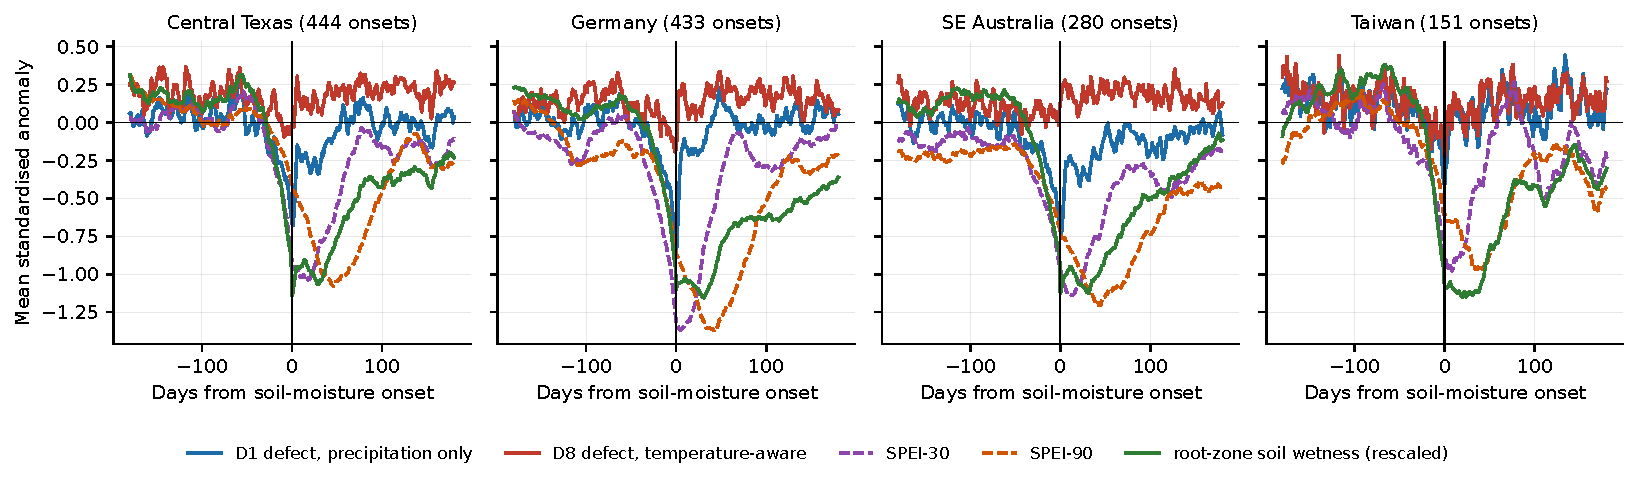
\includegraphics[width=\textwidth]{event_composites_mv.pdf}
\caption{Temperature-aware subset (\mvnst\ stations): mean anomalies aligned on reference onsets.
The temperature-aware defect (D8) responds much less at onset than the precipitation-only defect (D1)
and SPEI}\label{fig:compositesmv}
\end{figure}

\FloatBarrier
% ======================================================================
\section{Discussion}\label{sec:discussion}
\subsection{What the evaluation shows}
The study separates three claims that are easily conflated. The first concerns forecasting: a
backward-coherence penalty smooths the recurrent state path by about a quarter without changing
next-day forecast error by more than a fraction of a percent. This is established by equivalence tests
on \nstall\ stations, and it holds for the temperature-aware networks too. The second concerns
monitoring: the defect of such a network carries a drought signal. It declines towards onset, clearly
in three of the four regions and only briefly in Taiwan; it is associated with SPI-3 in every region and with soil moisture beyond SPI-3
in three; it alarms before SPI-90 when both detect an onset; and, pooled over regions, it detects more
onsets than monthly SPI-3. The third concerns added value, and
here the evidence is negative. At a matched alarm budget the defect detects fewer onsets than daily
SPI-90 or SPI-30, its timing advantage over SPI-90 is mostly reproduced by SPI-30, and it adds no
predictive information once SPI-30 is known. Most importantly for the method, the regularisation is not what makes
the defect work: the unregularised ablation performs indistinguishably. A smoother state path did not translate
into a better monitoring statistic.

One explanation is consistent with these results, although we did not test it directly. A recurrent
network that sees a 30-day window encodes recent precipitation; when a dry spell sets in, its state may
move towards the region of state space reached under near-zero input, where backward reconstruction is
easy, and the defect falls. On this reading the defect is a nonlinear, short-memory summary of recent
precipitation. The results show it to be comparable in timing to SPI-30 but less sensitive, possibly
because the network was trained to forecast tomorrow's rain rather than to measure deficits. The penalty
constrains how the state moves rather than what it encodes, which would explain why the ablation
behaves the same.

The temperature-aware extension is consistent with this reading. Giving the network temperature and
evaporative demand, and asking it to forecast evaporative demand as well, made it a better precipitation
forecaster but a worse monitor. A plausible but untested explanation is that its state now tracks
several slowly varying, seasonally structured inputs, so that a dry spell no longer drives it to a
distinctive, easily reconstructed configuration. In addition, the reference level of the defect drifted
upwards out of sample, together with warmer 2-m temperatures but in Texas and Germany already in
1991--2000, and a monitor standardised on 1961--1990 does not adjust for such drift. In this case,
giving the learned state more drought-relevant inputs did not make it a better drought statistic; what
the state encodes is shaped by its training objective, which here is forecasting.

\subsection{Implications for learned monitoring statistics}
The design choices that changed our conclusions relative to the exploratory study are not specific to
this method. Using
an independently defined event set rather than one detector's alarm as the reference avoids rewarding
whichever detector is fastest. Matching alarm budgets prevents a detector from appearing earlier
because it alarms more often; nominal ARL calibration on autocorrelated, seasonal data need not
equalise alarm rates. Comparing timing on jointly detected events avoids selection effects. Including
the ablation and a comparator with the same time scale as the learned model's memory exposes whether a
learned statistic contributes more than its receptive field. Resampling years rather than station-events
matters: here the year-cluster intervals for POD were \ciratiolo--\ciratiohi\ times as wide as naive
binomial intervals within regions, and \ciratioall\ times as wide for the pooled defect. These elements
can be applied unchanged to other learned monitoring statistics, such as autoencoder reconstruction
errors or forecast residuals of deep models.

The constructive outcome is modest. Combining the defect with SPI-90 kept SPI-90's sensitivity and
advanced alarms by a median of \dtimallDsixDthree\ days; SPI-30 achieves much the same. Where SPI at
several time scales is already computed, our results give no reason to add a learned hidden-state
statistic of this kind. Supplying the network with temperature and evaporative demand, the information
that SPEI adds to SPI \citep{vicenteserrano2010}, did not change this conclusion. A learned statistic
might help if the network were trained for the monitoring task itself, for example to predict future
deficits or a drought indicator, rather than tomorrow's rainfall; that is a different method, not
tested here, and would need its own pre-specified evaluation.

\subsection{Limitations}\label{sec:limits}
The reference events come from reanalysis soil moisture, which is a model product partly forced by
precipitation. This may favour precipitation-based detectors, and not necessarily equally, since their
time scales may match the memory of the reanalysis land-surface model to different degrees; it also
targets agricultural rather than hydrological drought; other references, such as streamflow or official
drought assessments like the U.S. Drought Monitor \citep{svoboda2002}, may rank detectors differently. The networks use one architecture with a 30-day window and 32 hidden units; longer windows or gated
cells could change the defect. The temperature-aware analysis covers \mvnst\ of the stations, uses donor
temperature records for some of them (in Australia a median of 82~km away), and estimates evaporative
demand by the temperature-only Hargreaves formula. The station networks differ in density, and Taiwan has only 13 stations
and 151 events, which makes its intervals wide. The direction of the CUSUM was pre-specified as
downward; an upward or two-sided rule was not evaluated. Finally, two analyses (SPI-30 and the
combination) were added after the primary results were seen and are labelled as post hoc; the
temperature-aware analysis was specified in a protocol amendment after those results were known but
before it was run.

\section{Conclusions}\label{sec:conclusion}
A backward-coherence penalty makes the hidden-state path of a recurrent precipitation model smoother
without affecting forecast accuracy, and the reconstruction defect of the model carries a drought
signal: it is associated with SPI-3, and in three of four regions with soil moisture, and it alarms
earlier than SPI-90 when both detect an onset. Under
a pre-specified evaluation with independent events, matched alarm budgets and dependence-aware
inference, however, the defect detects fewer droughts than daily SPI, its speed is largely that of a
30-day precipitation summary, and the regularisation does not improve it. Giving the network temperature
and evaporative demand improves its forecasts but weakens its defect relative to SPEI. Learned monitoring
statistics
should be evaluated against indices of matching time scale and against their own ablations before
operational value is claimed.

% ======================================================================
\FloatBarrier
\backmatter

\bmhead{Supplementary information}
Online Resource 1 (PDF) contains warning results at alternative alarm budgets, additional results of
the temperature-aware analysis, calibration diagnostics and a description of the code and data.

\bmhead{Acknowledgements}
This work was partially supported by the National Science and Technology Council, Taiwan (grant
115-2118-M-001-004-), and by the Institute of Statistical Science, Academia Sinica.

\begin{appendices}
\section{Pre-specified protocol and deviations}\label{app:protocol}
The protocol (file \texttt{PROTOCOL.md} in the code archive) fixed the data rules, periods, models,
detectors D1--D5, the calibration rule, the event definition, the scoring windows, the bootstrap and the
secondary analyses before any network was trained. Deviations, in chronological order: (1) before any
evaluation, the warm-up was shortened from five to three epochs and RMRNN checkpoints were made eligible
only once the penalty is active, after a pilot on one station showed that early stopping otherwise
selected warm-up checkpoints, making the regularised network identical to its ablation; (2) before any
evaluation, the covariate source changed from ERA5-Land to MERRA-2 (NASA POWER) because of access rate
limits, so soil-moisture percentiles use 1981--2024; (3) after the primary results, SPI-30 (D7) and the
combination D6 were added and are labelled post hoc; (4) the calibration grid search returns the grid
value whose calibration rate is closest to the budget, and unattainable budgets are flagged.
Amendment~1, written after the results above were known and before any temperature data were processed,
specified the temperature-aware analysis of Section~\ref{sec:mv_methods}: the temperature completeness and
donor rule, Hargreaves evapotranspiration, the network inputs and targets, detectors D8--D11, the primary
comparisons and the secondary analyses. Its only deviation is that the SPEI log-logistic parameters are
estimated by probability-weighted moments, the estimator of \citet{vicenteserrano2010}, instead of maximum
likelihood, because in a pilot on one station the maximum-likelihood fit gave reference-period SPEI with
mean 0.80 and standard deviation 0.48. The drift check in Online Resource 1, Table~\ref{S-tab:drift} is
descriptive and post hoc.
\end{appendices}

\bibliography{refs}

\section*{Statements and Declarations}
\paragraph{Funding} This work was partially supported by the National Science and Technology Council,
Taiwan (grant number 115-2118-M-001-004-).

\paragraph{Competing interests} The authors have no relevant financial or non-financial interests to
disclose.

\paragraph{Author contributions} Hui-Mean Foo: data curation, formal analysis, validation, writing
(review and editing). Yuan-chin Ivan Chang: conceptualisation, methodology, software, formal analysis,
writing (original draft). Both authors read and approved the final manuscript.

\paragraph{Data availability} All data analysed are publicly available: GHCN-Daily precipitation and
temperature \citep{ghcnd_data}, the Central Weather Administration station records rebuilt in the
Raingel archive \citep{raingel_data}, and MERRA-2 covariates through the NASA POWER archive
\citep{nasapower_data}. Station lists, reference events and all result tables are included in the code
repository, together with scripts that download and assemble the inputs.

\paragraph{Code availability} The code that reproduces every number, table and figure, with the
pre-specified protocol and its deviation log, is available at \url{https://github.com/knight-ivan/rmrnn-drought-monitoring} and will be made
public upon acceptance.


\end{document}
